%*************************************************************************
% A Classic Thesis Style
% An Homage to The Elements of Typographic Style
%
% Copyright (C) 2017 André Miede and Ivo Pletikosić
%
% If you like the style then I would appreciate a postcard. My address
% can be found in the file ClassicThesis.pdf. A collection of the
% postcards I received so far is available online at
% http://postcards.miede.de
%
% License:
% This program is free software; you can redistribute it and/or modify
% it under the terms of the GNU General Public License as published by
% the Free Software Foundation; either version 2 of the License, or
% (at your option) any later version.
%
% This program is distributed in the hope that it will be useful,
% but WITHOUT ANY WARRANTY; without even the implied warranty of
% MERCHANTABILITY or FITNESS FOR A PARTICULAR PURPOSE.  See the
% GNU General Public License for more details.
%
% You should have received a copy of the GNU General Public License
% along with this program; see the file COPYING.  If not, write to
% the Free Software Foundation, Inc., 59 Temple Place - Suite 330,
% Boston, MA 02111-1307, USA.
%
% PLEASE SEE ALSO THE AUTHORS' NOTE REGARDING THIS LICENSE
% IN THE DOCUMENTATION (ClassicThesis.pdf --> Chapter 1 / Chapter01.tex)
%*************************************************************************
\RequirePackage{silence} % :-\
    \WarningFilter{scrreprt}{Usage of package `titlesec'}
    %\WarningFilter{scrreprt}{Activating an ugly workaround}
    \WarningFilter{titlesec}{Non standard sectioning command detected}
\documentclass[ openright,titlepage,numbers=noenddot,headinclude,%twoside, %1headlines,% letterpaper a4paper
                footinclude=true,cleardoublepage=empty,abstractoff, % <--- obsolete, remove (todo)
                BCOR=5mm,paper=a4,fontsize=11pt,%11pt,a4paper,%
                ngerman,american,%lockflag%
                ]{scrreprt}

%*************************************************************************
% Note: Make all your adjustments in here
%*************************************************************************
% ****************************************************************************************************
% hdathesis-config.tex 
% Use it at the beginning of your thesis.tex, or as a LaTeX Preamble 
% in your thesis.{tex,lyx} with % ****************************************************************************************************
% hdathesis-config.tex 
% Use it at the beginning of your thesis.tex, or as a LaTeX Preamble 
% in your thesis.{tex,lyx} with % ****************************************************************************************************
% hdathesis-config.tex 
% Use it at the beginning of your thesis.tex, or as a LaTeX Preamble 
% in your thesis.{tex,lyx} with \input{hdathesis-config}
% ****************************************************************************************************

% ****************************************************************************************************
% 1. Personal data and user ad-hoc commands
% ****************************************************************************************************
\newcommand{\myTitle}{Bridging Legacy and Modern Systems: A Kafkaesque Approach to Adabas Data Replication\xspace}
%\newcommand{\mySubtitle}{An Homage to The Elements of Typographic Style\xspace}
\newcommand{\myDegree}{Bachelor of Science (B.Sc.)\xspace} 
%\newcommand{\myDegree}{Bachelor of Arts (B.A.)\xspace}
%\newcommand{\myDegree}{Master of Science (M.Sc.)\xspace}
%\newcommand{\myDegree}{Master of Arts (M.A.)\xspace}
\newcommand{\myName}{Leah Iliyav\xspace}
\newcommand{\myId}{1112407\xspace}
\newcommand{\myProf}{Prof. Dr. Oliver Weissmann\xspace}
\newcommand{\myOtherProf}{Prof. Dr. Michael von Rüden \xspace}
\newcommand{\myFaculty}{Fachbereich Informatik\xspace}
\newcommand{\myUni}{Hochschule Darmstadt\xspace}
\newcommand{\myLocation}{Darmstadt\xspace}
\newcommand{\myTime}{March 2025\xspace}
\newcommand{\myVersion}{version 1.0\xspace}

% ****************************************************************************************************
% 2. Is it a master thesis?
% ****************************************************************************************************
%\PassOptionsToPackage{master}{hdahesis} % uncomment if this is a master thesis 

% ****************************************************************************************************
% 3. Does the thesis have a lock flag?
% ****************************************************************************************************
%\PassOptionsToPackage{lockflag}{hdathesis} % uncomment if this thesis has a lock flag 

% ****************************************************************************************************
% 4. Loading some handy packages
% ****************************************************************************************************
% ****************************************************************************************************
% Packages with options that might require adjustments
% ****************************************************************************************************

%\PassOptionsToPackage{ngerman,american}{babel}   % change this to your language(s)
% Spanish languages need extra options in order to work with this template
%\PassOptionsToPackage{spanish,es-lcroman}{babel}
\usepackage{babel}


% ****************************************************************************************************

% ****************************************************************************************************
% 1. Personal data and user ad-hoc commands
% ****************************************************************************************************
\newcommand{\myTitle}{Bridging Legacy and Modern Systems: A Kafkaesque Approach to Adabas Data Replication\xspace}
%\newcommand{\mySubtitle}{An Homage to The Elements of Typographic Style\xspace}
\newcommand{\myDegree}{Bachelor of Science (B.Sc.)\xspace} 
%\newcommand{\myDegree}{Bachelor of Arts (B.A.)\xspace}
%\newcommand{\myDegree}{Master of Science (M.Sc.)\xspace}
%\newcommand{\myDegree}{Master of Arts (M.A.)\xspace}
\newcommand{\myName}{Leah Iliyav\xspace}
\newcommand{\myId}{1112407\xspace}
\newcommand{\myProf}{Prof. Dr. Oliver Weissmann\xspace}
\newcommand{\myOtherProf}{Prof. Dr. Michael von Rüden \xspace}
\newcommand{\myFaculty}{Fachbereich Informatik\xspace}
\newcommand{\myUni}{Hochschule Darmstadt\xspace}
\newcommand{\myLocation}{Darmstadt\xspace}
\newcommand{\myTime}{March 2025\xspace}
\newcommand{\myVersion}{version 1.0\xspace}

% ****************************************************************************************************
% 2. Is it a master thesis?
% ****************************************************************************************************
%\PassOptionsToPackage{master}{hdahesis} % uncomment if this is a master thesis 

% ****************************************************************************************************
% 3. Does the thesis have a lock flag?
% ****************************************************************************************************
%\PassOptionsToPackage{lockflag}{hdathesis} % uncomment if this thesis has a lock flag 

% ****************************************************************************************************
% 4. Loading some handy packages
% ****************************************************************************************************
% ****************************************************************************************************
% Packages with options that might require adjustments
% ****************************************************************************************************

%\PassOptionsToPackage{ngerman,american}{babel}   % change this to your language(s)
% Spanish languages need extra options in order to work with this template
%\PassOptionsToPackage{spanish,es-lcroman}{babel}
\usepackage{babel}


% ****************************************************************************************************

% ****************************************************************************************************
% 1. Personal data and user ad-hoc commands
% ****************************************************************************************************
\newcommand{\myTitle}{Bridging Legacy and Modern Systems: A Kafkaesque Approach to Adabas Data Replication\xspace}
%\newcommand{\mySubtitle}{An Homage to The Elements of Typographic Style\xspace}
\newcommand{\myDegree}{Bachelor of Science (B.Sc.)\xspace} 
%\newcommand{\myDegree}{Bachelor of Arts (B.A.)\xspace}
%\newcommand{\myDegree}{Master of Science (M.Sc.)\xspace}
%\newcommand{\myDegree}{Master of Arts (M.A.)\xspace}
\newcommand{\myName}{Leah Iliyav\xspace}
\newcommand{\myId}{1112407\xspace}
\newcommand{\myProf}{Prof. Dr. Oliver Weissmann\xspace}
\newcommand{\myOtherProf}{Prof. Dr. Michael von Rüden \xspace}
\newcommand{\myFaculty}{Fachbereich Informatik\xspace}
\newcommand{\myUni}{Hochschule Darmstadt\xspace}
\newcommand{\myLocation}{Darmstadt\xspace}
\newcommand{\myTime}{March 2025\xspace}
\newcommand{\myVersion}{version 1.0\xspace}

% ****************************************************************************************************
% 2. Is it a master thesis?
% ****************************************************************************************************
%\PassOptionsToPackage{master}{hdahesis} % uncomment if this is a master thesis 

% ****************************************************************************************************
% 3. Does the thesis have a lock flag?
% ****************************************************************************************************
%\PassOptionsToPackage{lockflag}{hdathesis} % uncomment if this thesis has a lock flag 

% ****************************************************************************************************
% 4. Loading some handy packages
% ****************************************************************************************************
% ****************************************************************************************************
% Packages with options that might require adjustments
% ****************************************************************************************************

%\PassOptionsToPackage{ngerman,american}{babel}   % change this to your language(s)
% Spanish languages need extra options in order to work with this template
%\PassOptionsToPackage{spanish,es-lcroman}{babel}
\usepackage{babel}


% ****************************************************************************************************
% classicthesis-config.tex
% formerly known as loadpackages.sty, classicthesis-ldpkg.sty, and classicthesis-preamble.sty
% Use it at the beginning of your ClassicThesis.tex, or as a LaTeX Preamble
% in your ClassicThesis.{tex,lyx} with % ****************************************************************************************************
% classicthesis-config.tex
% formerly known as loadpackages.sty, classicthesis-ldpkg.sty, and classicthesis-preamble.sty
% Use it at the beginning of your ClassicThesis.tex, or as a LaTeX Preamble
% in your ClassicThesis.{tex,lyx} with % ****************************************************************************************************
% classicthesis-config.tex
% formerly known as loadpackages.sty, classicthesis-ldpkg.sty, and classicthesis-preamble.sty
% Use it at the beginning of your ClassicThesis.tex, or as a LaTeX Preamble
% in your ClassicThesis.{tex,lyx} with \input{classicthesis-config}
% ****************************************************************************************************
% If you like the classicthesis, then I would appreciate a postcard.
% My address can be found in the file ClassicThesis.pdf. A collection
% of the postcards I received so far is available online at
% http://postcards.miede.de
% ****************************************************************************************************


% ****************************************************************************************************
% 0. Set the encoding of your files. UTF-8 is the only sensible encoding nowadays. If you can't read
% äöüßáéçèê∂åëæƒÏ€ then change the encoding setting in your editor, not the line below. If your editor
% does not support utf8 use another editor!
% ****************************************************************************************************
\PassOptionsToPackage{utf8}{inputenc}
  \usepackage{inputenc}

% ****************************************************************************************************
% 1. Configure classicthesis for your needs here, e.g., remove "drafting" below
% in order to deactivate the time-stamp on the pages
% (see ClassicThesis.pdf for more information):
% ****************************************************************************************************
\PassOptionsToPackage{
  drafting=false,   % print version information on the bottom of the pages
  tocaligned=false, % the left column of the toc will be aligned (no indentation)
  dottedtoc=true,   % page numbers in ToC flushed right
  parts=true,       % use part division
  eulerchapternumbers=true, % use AMS Euler for chapter font (otherwise Palatino)
  linedheaders=false,       % chaper headers will have line above and beneath
  floatperchapter=true,     % numbering per chapter for all floats (i.e., Figure 1.1)
  listings=true,    % load listings package and setup LoL
  subfig=true,      % setup for preloaded subfig package
  eulermath=false,  % use awesome Euler fonts for mathematical formulae (only with pdfLaTeX)
  beramono=true,    % toggle a nice monospaced font (w/ bold)
  minionpro=false   % setup for minion pro font; use minion pro small caps as well (only with pdfLaTeX)
}{classicthesis}


% ****************************************************************************************************
% 2. Personal data and user ad-hoc commands
% ****************************************************************************************************
%\newcommand{\myTitle}{A Classic Thesis Style\xspace}
%\newcommand{\mySubtitle}{An Homage to The Elements of Typographic Style\xspace}
%\newcommand{\myDegree}{Doktor-Ingenieur (Dr.-Ing.)\xspace}
%\newcommand{\myName}{André Miede\xspace}
%\newcommand{\myProf}{Put name here\xspace}
%\newcommand{\myOtherProf}{Put name here\xspace}
%\newcommand{\mySupervisor}{Put name here\xspace}
%\newcommand{\myFaculty}{Put data here\xspace}
%\newcommand{\myDepartment}{Put data here\xspace}
%\newcommand{\myUni}{Put data here\xspace}
%\newcommand{\myLocation}{Saarbrücken\xspace}
%\newcommand{\myTime}{October 2017\xspace}
%\newcommand{\myVersion}{version 4.4}

% ********************************************************************
% Setup, finetuning, and useful commands
% ********************************************************************
\newcounter{dummy} % necessary for correct hyperlinks (to index, bib, etc.)
\newlength{\abcd} % for ab..z string length calculation
\providecommand{\mLyX}{L\kern-.1667em\lower.25em\hbox{Y}\kern-.125emX\@}
\newcommand{\ie}{i.\,e.}
\newcommand{\Ie}{I.\,e.}
\newcommand{\eg}{e.\,g.}
\newcommand{\Eg}{E.\,g.}
% ****************************************************************************************************


% ****************************************************************************************************
% 3. Loading some handy packages
% ****************************************************************************************************
% ********************************************************************
% Packages with options that might require adjustments
% ********************************************************************
%\PassOptionsToPackage{ngerman,american}{babel}   % change this to your language(s), main language last
% Spanish languages need extra options in order to work with this template
%\PassOptionsToPackage{spanish,es-lcroman}{babel}
\usepackage{babel}

\usepackage{csquotes}

\PassOptionsToPackage{%
  %backend=biber,bibencoding=utf8, %instead of bibtex
  backend=bibtex8,bibencoding=ascii,%
  language=auto,%
  %style=numeric-comp,%
  style=alphabetic,%
  %style=authoryear-comp, % Author 1999, 2010
  %bibstyle=authoryear,dashed=false, % dashed: substitute rep. author with ---
  sorting=nyt, % name, year, title
  maxbibnames=10, % default: 3, et al.
  %backref=true,%
  natbib=true % natbib compatibility mode (\citep and \citet still work)
}{biblatex}
  \usepackage{biblatex}

\PassOptionsToPackage{fleqn}{amsmath}       % math environments and more by the AMS
  \usepackage{amsmath}

\PassOptionsToPackage{doublespacing}{hdathesis}  % options: abbrev exam big wiwi english master
  \usepackage{hdathesis}

% ********************************************************************
% General useful packages
% ********************************************************************
\PassOptionsToPackage{T1}{fontenc} % T2A for cyrillics
  \usepackage{fontenc}
\usepackage{textcomp} % fix warning with missing font shapes
\usepackage{scrhack} % fix warnings when using KOMA with listings package
\usepackage{xspace} % to get the spacing after macros right
\usepackage{mparhack} % get marginpar right
%\usepackage{fixltx2e} % fixes some LaTeX stuff --> since 2015 in the LaTeX kernel (see below)
% \usepackage[latest]{latexrelease} % emulate newer kernel version if older is detected
\PassOptionsToPackage{printonlyused,smaller}{acronym}
  \usepackage{acronym} % nice macros for handling all acronyms in the thesis
  %\renewcommand{\bflabel}[1]{{#1}\hfill} % fix the list of acronyms --> no longer working
  %\renewcommand*{\acsfont}[1]{\textsc{#1}}
  %\renewcommand*{\aclabelfont}[1]{\acsfont{#1}}
  %\def\bflabel#1{{#1\hfill}}
  \def\bflabel#1{{\acsfont{#1}\hfill}}
  \def\aclabelfont#1{\acsfont{#1}}
% ****************************************************************************************************
%\usepackage{pgfplots} % External TikZ/PGF support (thanks to Andreas Nautsch)
%\usetikzlibrary{external}
%\tikzexternalize[mode=list and make, prefix=ext-tikz/]
% ****************************************************************************************************


% ****************************************************************************************************
% 4. Setup floats: tables, (sub)figures, and captions
% ****************************************************************************************************
\usepackage{tabularx} % better tables
  \setlength{\extrarowheight}{3pt} % increase table row height
\newcommand{\tableheadline}[1]{\multicolumn{1}{c}{\spacedlowsmallcaps{#1}}}
\newcommand{\myfloatalign}{\centering} % to be used with each float for alignment
\usepackage{caption}
% Thanks to cgnieder and Claus Lahiri
% http://tex.stackexchange.com/questions/69349/spacedlowsmallcaps-in-caption-label
% [REMOVED DUE TO OTHER PROBLEMS, SEE ISSUE #82]
%\DeclareCaptionLabelFormat{smallcaps}{\bothIfFirst{#1}{~}\MakeTextLowercase{\textsc{#2}}}
%\captionsetup{font=small,labelformat=smallcaps} % format=hang,
\captionsetup{font=small} % format=hang,
\usepackage{subfig}
% ****************************************************************************************************


% ****************************************************************************************************
% 5. Setup code listings
% ****************************************************************************************************
\usepackage{listings}
%\lstset{emph={trueIndex,root},emphstyle=\color{BlueViolet}}%\underbar} % for special keywords
\lstset{language=[LaTeX]Tex,%C++,
  morekeywords={PassOptionsToPackage,selectlanguage},
  keywordstyle=\color{RoyalBlue},%\bfseries,
  basicstyle=\small\ttfamily,
  %identifierstyle=\color{NavyBlue},
  commentstyle=\color{Green}\ttfamily,
  stringstyle=\rmfamily,
  numbers=none,%left,%
  numberstyle=\scriptsize,%\tiny
  stepnumber=5,
  numbersep=8pt,
  showstringspaces=false,
  breaklines=true,
  %frameround=ftff,
  %frame=single,
  belowcaptionskip=.75\baselineskip
  %frame=L
}
% ****************************************************************************************************


% ****************************************************************************************************
% 6. PDFLaTeX, hyperreferences, and citation backreferences
% ****************************************************************************************************
% ********************************************************************
% Using PDFLaTeX
% ********************************************************************
\PassOptionsToPackage{hyperfootnotes=false,pdfpagelabels}{hyperref}
  \usepackage{hyperref}  % backref linktocpage pagebackref
%\ifpdf
%\pdfcompresslevel=9
%\pdfadjustspacing=1
%\fi
%\PassOptionsToPackage{pdftex}{graphicx} %%%IVO: driver will be chosen automatically
  \usepackage{graphicx}


% ********************************************************************
% Hyperreferences
% ********************************************************************
\hypersetup{%
  %draft, % hyperref's draft mode, for printing see below
  colorlinks=true, linktocpage=true, pdfstartpage=3, pdfstartview=FitV,%
  % uncomment the following line if you want to have black links (e.g., for printing)
  %colorlinks=false, linktocpage=false, pdfstartpage=3, pdfstartview=FitV, pdfborder={0 0 0},%
  breaklinks=true, pdfpagemode=UseNone, pageanchor=true, pdfpagemode=UseOutlines,%
  plainpages=false, bookmarksnumbered, bookmarksopen=true, bookmarksopenlevel=1,%
  hypertexnames=true, pdfhighlight=/O,%nesting=true,%frenchlinks,%
  urlcolor=webbrown, linkcolor=RoyalBlue, citecolor=webgreen, %pagecolor=RoyalBlue,%
  %urlcolor=Black, linkcolor=Black, citecolor=Black, %pagecolor=Black,%
  pdftitle={\myTitle},%
  pdfauthor={\textcopyright\ \myName, \myUni, \myFaculty},%
  pdfsubject={},%
  pdfkeywords={},%
  pdfcreator={pdfLaTeX},%
  pdfproducer={LaTeX with hyperref and classicthesis}%
}

% ********************************************************************
% Setup autoreferences
% ********************************************************************
% There are some issues regarding autorefnames
% http://www.ureader.de/msg/136221647.aspx
% http://www.tex.ac.uk/cgi-bin/texfaq2html?label=latexwords
% you have to redefine the makros for the
% language you use, e.g., american, ngerman
% (as chosen when loading babel/AtBeginDocument)
% ********************************************************************
\makeatletter
\@ifpackageloaded{babel}%
  {%
    \addto\extrasamerican{%
      \renewcommand*{\figureautorefname}{Figure}%
      \renewcommand*{\tableautorefname}{Table}%
      \renewcommand*{\partautorefname}{Part}%
      \renewcommand*{\chapterautorefname}{Chapter}%
      \renewcommand*{\sectionautorefname}{Section}%
      \renewcommand*{\subsectionautorefname}{Section}%
      \renewcommand*{\subsubsectionautorefname}{Section}%
    }%
    \addto\extrasngerman{%
      \renewcommand*{\paragraphautorefname}{Absatz}%
      \renewcommand*{\subparagraphautorefname}{Unterabsatz}%
      \renewcommand*{\footnoteautorefname}{Fu\"snote}%
      \renewcommand*{\FancyVerbLineautorefname}{Zeile}%
      \renewcommand*{\theoremautorefname}{Theorem}%
      \renewcommand*{\appendixautorefname}{Anhang}%
      \renewcommand*{\equationautorefname}{Gleichung}%
      \renewcommand*{\itemautorefname}{Punkt}%
    }%
      % Fix to getting autorefs for subfigures right (thanks to Belinda Vogt for changing the definition)
      \providecommand{\subfigureautorefname}{\figureautorefname}%
    }{\relax}
\makeatother


% ****************************************************************************************************
% 7. Last calls before the bar closes
% ****************************************************************************************************
% ********************************************************************
% Development Stuff
% ********************************************************************
\listfiles
%\PassOptionsToPackage{l2tabu,orthodox,abort}{nag}
%  \usepackage{nag}
%\PassOptionsToPackage{warning, all}{onlyamsmath}
%  \usepackage{onlyamsmath}

% ********************************************************************
% Last, but not least...
% ********************************************************************
\usepackage{classicthesis}
% ****************************************************************************************************


% ****************************************************************************************************
% 8. Further adjustments (experimental)
% ****************************************************************************************************
% ********************************************************************
% Changing the text area
% ********************************************************************
%\areaset[current]{312pt}{761pt} % 686 (factor 2.2) + 33 head + 42 head \the\footskip
%\setlength{\marginparwidth}{7em}%
%\setlength{\marginparsep}{2em}%

% ********************************************************************
% Using different fonts
% ********************************************************************
%\usepackage[oldstylenums]{kpfonts} % oldstyle notextcomp
%\usepackage[osf]{libertine}
%\usepackage[light,condensed,math]{iwona}
%\renewcommand{\sfdefault}{iwona}
%\usepackage{lmodern} % <-- no osf support :-(
%\usepackage{cfr-lm} %
%\usepackage[urw-garamond]{mathdesign} <-- no osf support :-(
%\usepackage[default,osfigures]{opensans} % scale=0.95
%\usepackage[sfdefault]{FiraSans}
% ********************************************************************
% \usepackage[largesc,osf]{newpxtext}
% Used to fix these:
% https://bitbucket.org/amiede/classicthesis/issues/139/italics-in-pallatino-capitals-chapter
% https://bitbucket.org/amiede/classicthesis/issues/45/problema-testatine-su-classicthesis-style
% ********************************************************************
%\linespread{1.05} % a bit more for Palatino
% ****************************************************************************************************

% ****************************************************************************************************
% If you like the classicthesis, then I would appreciate a postcard.
% My address can be found in the file ClassicThesis.pdf. A collection
% of the postcards I received so far is available online at
% http://postcards.miede.de
% ****************************************************************************************************


% ****************************************************************************************************
% 0. Set the encoding of your files. UTF-8 is the only sensible encoding nowadays. If you can't read
% äöüßáéçèê∂åëæƒÏ€ then change the encoding setting in your editor, not the line below. If your editor
% does not support utf8 use another editor!
% ****************************************************************************************************
\PassOptionsToPackage{utf8}{inputenc}
  \usepackage{inputenc}

% ****************************************************************************************************
% 1. Configure classicthesis for your needs here, e.g., remove "drafting" below
% in order to deactivate the time-stamp on the pages
% (see ClassicThesis.pdf for more information):
% ****************************************************************************************************
\PassOptionsToPackage{
  drafting=false,   % print version information on the bottom of the pages
  tocaligned=false, % the left column of the toc will be aligned (no indentation)
  dottedtoc=true,   % page numbers in ToC flushed right
  parts=true,       % use part division
  eulerchapternumbers=true, % use AMS Euler for chapter font (otherwise Palatino)
  linedheaders=false,       % chaper headers will have line above and beneath
  floatperchapter=true,     % numbering per chapter for all floats (i.e., Figure 1.1)
  listings=true,    % load listings package and setup LoL
  subfig=true,      % setup for preloaded subfig package
  eulermath=false,  % use awesome Euler fonts for mathematical formulae (only with pdfLaTeX)
  beramono=true,    % toggle a nice monospaced font (w/ bold)
  minionpro=false   % setup for minion pro font; use minion pro small caps as well (only with pdfLaTeX)
}{classicthesis}


% ****************************************************************************************************
% 2. Personal data and user ad-hoc commands
% ****************************************************************************************************
%\newcommand{\myTitle}{A Classic Thesis Style\xspace}
%\newcommand{\mySubtitle}{An Homage to The Elements of Typographic Style\xspace}
%\newcommand{\myDegree}{Doktor-Ingenieur (Dr.-Ing.)\xspace}
%\newcommand{\myName}{André Miede\xspace}
%\newcommand{\myProf}{Put name here\xspace}
%\newcommand{\myOtherProf}{Put name here\xspace}
%\newcommand{\mySupervisor}{Put name here\xspace}
%\newcommand{\myFaculty}{Put data here\xspace}
%\newcommand{\myDepartment}{Put data here\xspace}
%\newcommand{\myUni}{Put data here\xspace}
%\newcommand{\myLocation}{Saarbrücken\xspace}
%\newcommand{\myTime}{October 2017\xspace}
%\newcommand{\myVersion}{version 4.4}

% ********************************************************************
% Setup, finetuning, and useful commands
% ********************************************************************
\newcounter{dummy} % necessary for correct hyperlinks (to index, bib, etc.)
\newlength{\abcd} % for ab..z string length calculation
\providecommand{\mLyX}{L\kern-.1667em\lower.25em\hbox{Y}\kern-.125emX\@}
\newcommand{\ie}{i.\,e.}
\newcommand{\Ie}{I.\,e.}
\newcommand{\eg}{e.\,g.}
\newcommand{\Eg}{E.\,g.}
% ****************************************************************************************************


% ****************************************************************************************************
% 3. Loading some handy packages
% ****************************************************************************************************
% ********************************************************************
% Packages with options that might require adjustments
% ********************************************************************
%\PassOptionsToPackage{ngerman,american}{babel}   % change this to your language(s), main language last
% Spanish languages need extra options in order to work with this template
%\PassOptionsToPackage{spanish,es-lcroman}{babel}
\usepackage{babel}

\usepackage{csquotes}

\PassOptionsToPackage{%
  %backend=biber,bibencoding=utf8, %instead of bibtex
  backend=bibtex8,bibencoding=ascii,%
  language=auto,%
  %style=numeric-comp,%
  style=alphabetic,%
  %style=authoryear-comp, % Author 1999, 2010
  %bibstyle=authoryear,dashed=false, % dashed: substitute rep. author with ---
  sorting=nyt, % name, year, title
  maxbibnames=10, % default: 3, et al.
  %backref=true,%
  natbib=true % natbib compatibility mode (\citep and \citet still work)
}{biblatex}
  \usepackage{biblatex}

\PassOptionsToPackage{fleqn}{amsmath}       % math environments and more by the AMS
  \usepackage{amsmath}

\PassOptionsToPackage{doublespacing}{hdathesis}  % options: abbrev exam big wiwi english master
  \usepackage{hdathesis}

% ********************************************************************
% General useful packages
% ********************************************************************
\PassOptionsToPackage{T1}{fontenc} % T2A for cyrillics
  \usepackage{fontenc}
\usepackage{textcomp} % fix warning with missing font shapes
\usepackage{scrhack} % fix warnings when using KOMA with listings package
\usepackage{xspace} % to get the spacing after macros right
\usepackage{mparhack} % get marginpar right
%\usepackage{fixltx2e} % fixes some LaTeX stuff --> since 2015 in the LaTeX kernel (see below)
% \usepackage[latest]{latexrelease} % emulate newer kernel version if older is detected
\PassOptionsToPackage{printonlyused,smaller}{acronym}
  \usepackage{acronym} % nice macros for handling all acronyms in the thesis
  %\renewcommand{\bflabel}[1]{{#1}\hfill} % fix the list of acronyms --> no longer working
  %\renewcommand*{\acsfont}[1]{\textsc{#1}}
  %\renewcommand*{\aclabelfont}[1]{\acsfont{#1}}
  %\def\bflabel#1{{#1\hfill}}
  \def\bflabel#1{{\acsfont{#1}\hfill}}
  \def\aclabelfont#1{\acsfont{#1}}
% ****************************************************************************************************
%\usepackage{pgfplots} % External TikZ/PGF support (thanks to Andreas Nautsch)
%\usetikzlibrary{external}
%\tikzexternalize[mode=list and make, prefix=ext-tikz/]
% ****************************************************************************************************


% ****************************************************************************************************
% 4. Setup floats: tables, (sub)figures, and captions
% ****************************************************************************************************
\usepackage{tabularx} % better tables
  \setlength{\extrarowheight}{3pt} % increase table row height
\newcommand{\tableheadline}[1]{\multicolumn{1}{c}{\spacedlowsmallcaps{#1}}}
\newcommand{\myfloatalign}{\centering} % to be used with each float for alignment
\usepackage{caption}
% Thanks to cgnieder and Claus Lahiri
% http://tex.stackexchange.com/questions/69349/spacedlowsmallcaps-in-caption-label
% [REMOVED DUE TO OTHER PROBLEMS, SEE ISSUE #82]
%\DeclareCaptionLabelFormat{smallcaps}{\bothIfFirst{#1}{~}\MakeTextLowercase{\textsc{#2}}}
%\captionsetup{font=small,labelformat=smallcaps} % format=hang,
\captionsetup{font=small} % format=hang,
\usepackage{subfig}
% ****************************************************************************************************


% ****************************************************************************************************
% 5. Setup code listings
% ****************************************************************************************************
\usepackage{listings}
%\lstset{emph={trueIndex,root},emphstyle=\color{BlueViolet}}%\underbar} % for special keywords
\lstset{language=[LaTeX]Tex,%C++,
  morekeywords={PassOptionsToPackage,selectlanguage},
  keywordstyle=\color{RoyalBlue},%\bfseries,
  basicstyle=\small\ttfamily,
  %identifierstyle=\color{NavyBlue},
  commentstyle=\color{Green}\ttfamily,
  stringstyle=\rmfamily,
  numbers=none,%left,%
  numberstyle=\scriptsize,%\tiny
  stepnumber=5,
  numbersep=8pt,
  showstringspaces=false,
  breaklines=true,
  %frameround=ftff,
  %frame=single,
  belowcaptionskip=.75\baselineskip
  %frame=L
}
% ****************************************************************************************************


% ****************************************************************************************************
% 6. PDFLaTeX, hyperreferences, and citation backreferences
% ****************************************************************************************************
% ********************************************************************
% Using PDFLaTeX
% ********************************************************************
\PassOptionsToPackage{hyperfootnotes=false,pdfpagelabels}{hyperref}
  \usepackage{hyperref}  % backref linktocpage pagebackref
%\ifpdf
%\pdfcompresslevel=9
%\pdfadjustspacing=1
%\fi
%\PassOptionsToPackage{pdftex}{graphicx} %%%IVO: driver will be chosen automatically
  \usepackage{graphicx}


% ********************************************************************
% Hyperreferences
% ********************************************************************
\hypersetup{%
  %draft, % hyperref's draft mode, for printing see below
  colorlinks=true, linktocpage=true, pdfstartpage=3, pdfstartview=FitV,%
  % uncomment the following line if you want to have black links (e.g., for printing)
  %colorlinks=false, linktocpage=false, pdfstartpage=3, pdfstartview=FitV, pdfborder={0 0 0},%
  breaklinks=true, pdfpagemode=UseNone, pageanchor=true, pdfpagemode=UseOutlines,%
  plainpages=false, bookmarksnumbered, bookmarksopen=true, bookmarksopenlevel=1,%
  hypertexnames=true, pdfhighlight=/O,%nesting=true,%frenchlinks,%
  urlcolor=webbrown, linkcolor=RoyalBlue, citecolor=webgreen, %pagecolor=RoyalBlue,%
  %urlcolor=Black, linkcolor=Black, citecolor=Black, %pagecolor=Black,%
  pdftitle={\myTitle},%
  pdfauthor={\textcopyright\ \myName, \myUni, \myFaculty},%
  pdfsubject={},%
  pdfkeywords={},%
  pdfcreator={pdfLaTeX},%
  pdfproducer={LaTeX with hyperref and classicthesis}%
}

% ********************************************************************
% Setup autoreferences
% ********************************************************************
% There are some issues regarding autorefnames
% http://www.ureader.de/msg/136221647.aspx
% http://www.tex.ac.uk/cgi-bin/texfaq2html?label=latexwords
% you have to redefine the makros for the
% language you use, e.g., american, ngerman
% (as chosen when loading babel/AtBeginDocument)
% ********************************************************************
\makeatletter
\@ifpackageloaded{babel}%
  {%
    \addto\extrasamerican{%
      \renewcommand*{\figureautorefname}{Figure}%
      \renewcommand*{\tableautorefname}{Table}%
      \renewcommand*{\partautorefname}{Part}%
      \renewcommand*{\chapterautorefname}{Chapter}%
      \renewcommand*{\sectionautorefname}{Section}%
      \renewcommand*{\subsectionautorefname}{Section}%
      \renewcommand*{\subsubsectionautorefname}{Section}%
    }%
    \addto\extrasngerman{%
      \renewcommand*{\paragraphautorefname}{Absatz}%
      \renewcommand*{\subparagraphautorefname}{Unterabsatz}%
      \renewcommand*{\footnoteautorefname}{Fu\"snote}%
      \renewcommand*{\FancyVerbLineautorefname}{Zeile}%
      \renewcommand*{\theoremautorefname}{Theorem}%
      \renewcommand*{\appendixautorefname}{Anhang}%
      \renewcommand*{\equationautorefname}{Gleichung}%
      \renewcommand*{\itemautorefname}{Punkt}%
    }%
      % Fix to getting autorefs for subfigures right (thanks to Belinda Vogt for changing the definition)
      \providecommand{\subfigureautorefname}{\figureautorefname}%
    }{\relax}
\makeatother


% ****************************************************************************************************
% 7. Last calls before the bar closes
% ****************************************************************************************************
% ********************************************************************
% Development Stuff
% ********************************************************************
\listfiles
%\PassOptionsToPackage{l2tabu,orthodox,abort}{nag}
%  \usepackage{nag}
%\PassOptionsToPackage{warning, all}{onlyamsmath}
%  \usepackage{onlyamsmath}

% ********************************************************************
% Last, but not least...
% ********************************************************************
\usepackage{classicthesis}
% ****************************************************************************************************


% ****************************************************************************************************
% 8. Further adjustments (experimental)
% ****************************************************************************************************
% ********************************************************************
% Changing the text area
% ********************************************************************
%\areaset[current]{312pt}{761pt} % 686 (factor 2.2) + 33 head + 42 head \the\footskip
%\setlength{\marginparwidth}{7em}%
%\setlength{\marginparsep}{2em}%

% ********************************************************************
% Using different fonts
% ********************************************************************
%\usepackage[oldstylenums]{kpfonts} % oldstyle notextcomp
%\usepackage[osf]{libertine}
%\usepackage[light,condensed,math]{iwona}
%\renewcommand{\sfdefault}{iwona}
%\usepackage{lmodern} % <-- no osf support :-(
%\usepackage{cfr-lm} %
%\usepackage[urw-garamond]{mathdesign} <-- no osf support :-(
%\usepackage[default,osfigures]{opensans} % scale=0.95
%\usepackage[sfdefault]{FiraSans}
% ********************************************************************
% \usepackage[largesc,osf]{newpxtext}
% Used to fix these:
% https://bitbucket.org/amiede/classicthesis/issues/139/italics-in-pallatino-capitals-chapter
% https://bitbucket.org/amiede/classicthesis/issues/45/problema-testatine-su-classicthesis-style
% ********************************************************************
%\linespread{1.05} % a bit more for Palatino
% ****************************************************************************************************

% ****************************************************************************************************
% If you like the classicthesis, then I would appreciate a postcard.
% My address can be found in the file ClassicThesis.pdf. A collection
% of the postcards I received so far is available online at
% http://postcards.miede.de
% ****************************************************************************************************


% ****************************************************************************************************
% 0. Set the encoding of your files. UTF-8 is the only sensible encoding nowadays. If you can't read
% äöüßáéçèê∂åëæƒÏ€ then change the encoding setting in your editor, not the line below. If your editor
% does not support utf8 use another editor!
% ****************************************************************************************************
\PassOptionsToPackage{utf8}{inputenc}
  \usepackage{inputenc}

% ****************************************************************************************************
% 1. Configure classicthesis for your needs here, e.g., remove "drafting" below
% in order to deactivate the time-stamp on the pages
% (see ClassicThesis.pdf for more information):
% ****************************************************************************************************
\PassOptionsToPackage{
  drafting=false,   % print version information on the bottom of the pages
  tocaligned=false, % the left column of the toc will be aligned (no indentation)
  dottedtoc=true,   % page numbers in ToC flushed right
  parts=true,       % use part division
  eulerchapternumbers=true, % use AMS Euler for chapter font (otherwise Palatino)
  linedheaders=false,       % chaper headers will have line above and beneath
  floatperchapter=true,     % numbering per chapter for all floats (i.e., Figure 1.1)
  listings=true,    % load listings package and setup LoL
  subfig=true,      % setup for preloaded subfig package
  eulermath=false,  % use awesome Euler fonts for mathematical formulae (only with pdfLaTeX)
  beramono=true,    % toggle a nice monospaced font (w/ bold)
  minionpro=false   % setup for minion pro font; use minion pro small caps as well (only with pdfLaTeX)
}{classicthesis}


% ****************************************************************************************************
% 2. Personal data and user ad-hoc commands
% ****************************************************************************************************
%\newcommand{\myTitle}{A Classic Thesis Style\xspace}
%\newcommand{\mySubtitle}{An Homage to The Elements of Typographic Style\xspace}
%\newcommand{\myDegree}{Doktor-Ingenieur (Dr.-Ing.)\xspace}
%\newcommand{\myName}{André Miede\xspace}
%\newcommand{\myProf}{Put name here\xspace}
%\newcommand{\myOtherProf}{Put name here\xspace}
%\newcommand{\mySupervisor}{Put name here\xspace}
%\newcommand{\myFaculty}{Put data here\xspace}
%\newcommand{\myDepartment}{Put data here\xspace}
%\newcommand{\myUni}{Put data here\xspace}
%\newcommand{\myLocation}{Saarbrücken\xspace}
%\newcommand{\myTime}{October 2017\xspace}
%\newcommand{\myVersion}{version 4.4}

% ********************************************************************
% Setup, finetuning, and useful commands
% ********************************************************************
\newcounter{dummy} % necessary for correct hyperlinks (to index, bib, etc.)
\newlength{\abcd} % for ab..z string length calculation
\providecommand{\mLyX}{L\kern-.1667em\lower.25em\hbox{Y}\kern-.125emX\@}
\newcommand{\ie}{i.\,e.}
\newcommand{\Ie}{I.\,e.}
\newcommand{\eg}{e.\,g.}
\newcommand{\Eg}{E.\,g.}
% ****************************************************************************************************


% ****************************************************************************************************
% 3. Loading some handy packages
% ****************************************************************************************************
% ********************************************************************
% Packages with options that might require adjustments
% ********************************************************************
%\PassOptionsToPackage{ngerman,american}{babel}   % change this to your language(s), main language last
% Spanish languages need extra options in order to work with this template
%\PassOptionsToPackage{spanish,es-lcroman}{babel}
\usepackage{babel}

\usepackage{csquotes}

\PassOptionsToPackage{%
  %backend=biber,bibencoding=utf8, %instead of bibtex
  backend=bibtex8,bibencoding=ascii,%
  language=auto,%
  %style=numeric-comp,%
  style=alphabetic,%
  %style=authoryear-comp, % Author 1999, 2010
  %bibstyle=authoryear,dashed=false, % dashed: substitute rep. author with ---
  sorting=nyt, % name, year, title
  maxbibnames=10, % default: 3, et al.
  %backref=true,%
  natbib=true % natbib compatibility mode (\citep and \citet still work)
}{biblatex}
  \usepackage{biblatex}

\PassOptionsToPackage{fleqn}{amsmath}       % math environments and more by the AMS
  \usepackage{amsmath}

\PassOptionsToPackage{doublespacing}{hdathesis}  % options: abbrev exam big wiwi english master
  \usepackage{hdathesis}

% ********************************************************************
% General useful packages
% ********************************************************************
\PassOptionsToPackage{T1}{fontenc} % T2A for cyrillics
  \usepackage{fontenc}
\usepackage{textcomp} % fix warning with missing font shapes
\usepackage{scrhack} % fix warnings when using KOMA with listings package
\usepackage{xspace} % to get the spacing after macros right
\usepackage{mparhack} % get marginpar right
%\usepackage{fixltx2e} % fixes some LaTeX stuff --> since 2015 in the LaTeX kernel (see below)
% \usepackage[latest]{latexrelease} % emulate newer kernel version if older is detected
\PassOptionsToPackage{printonlyused,smaller}{acronym}
  \usepackage{acronym} % nice macros for handling all acronyms in the thesis
  %\renewcommand{\bflabel}[1]{{#1}\hfill} % fix the list of acronyms --> no longer working
  %\renewcommand*{\acsfont}[1]{\textsc{#1}}
  %\renewcommand*{\aclabelfont}[1]{\acsfont{#1}}
  %\def\bflabel#1{{#1\hfill}}
  \def\bflabel#1{{\acsfont{#1}\hfill}}
  \def\aclabelfont#1{\acsfont{#1}}
% ****************************************************************************************************
%\usepackage{pgfplots} % External TikZ/PGF support (thanks to Andreas Nautsch)
%\usetikzlibrary{external}
%\tikzexternalize[mode=list and make, prefix=ext-tikz/]
% ****************************************************************************************************


% ****************************************************************************************************
% 4. Setup floats: tables, (sub)figures, and captions
% ****************************************************************************************************
\usepackage{tabularx} % better tables
  \setlength{\extrarowheight}{3pt} % increase table row height
\newcommand{\tableheadline}[1]{\multicolumn{1}{c}{\spacedlowsmallcaps{#1}}}
\newcommand{\myfloatalign}{\centering} % to be used with each float for alignment
\usepackage{caption}
% Thanks to cgnieder and Claus Lahiri
% http://tex.stackexchange.com/questions/69349/spacedlowsmallcaps-in-caption-label
% [REMOVED DUE TO OTHER PROBLEMS, SEE ISSUE #82]
%\DeclareCaptionLabelFormat{smallcaps}{\bothIfFirst{#1}{~}\MakeTextLowercase{\textsc{#2}}}
%\captionsetup{font=small,labelformat=smallcaps} % format=hang,
\captionsetup{font=small} % format=hang,
\usepackage{subfig}
% ****************************************************************************************************


% ****************************************************************************************************
% 5. Setup code listings
% ****************************************************************************************************
\usepackage{listings}
%\lstset{emph={trueIndex,root},emphstyle=\color{BlueViolet}}%\underbar} % for special keywords
\lstset{language=[LaTeX]Tex,%C++,
  morekeywords={PassOptionsToPackage,selectlanguage},
  keywordstyle=\color{RoyalBlue},%\bfseries,
  basicstyle=\small\ttfamily,
  %identifierstyle=\color{NavyBlue},
  commentstyle=\color{Green}\ttfamily,
  stringstyle=\rmfamily,
  numbers=none,%left,%
  numberstyle=\scriptsize,%\tiny
  stepnumber=5,
  numbersep=8pt,
  showstringspaces=false,
  breaklines=true,
  %frameround=ftff,
  %frame=single,
  belowcaptionskip=.75\baselineskip
  %frame=L
}
% ****************************************************************************************************


% ****************************************************************************************************
% 6. PDFLaTeX, hyperreferences, and citation backreferences
% ****************************************************************************************************
% ********************************************************************
% Using PDFLaTeX
% ********************************************************************
\PassOptionsToPackage{hyperfootnotes=false,pdfpagelabels}{hyperref}
  \usepackage{hyperref}  % backref linktocpage pagebackref
%\ifpdf
%\pdfcompresslevel=9
%\pdfadjustspacing=1
%\fi
%\PassOptionsToPackage{pdftex}{graphicx} %%%IVO: driver will be chosen automatically
  \usepackage{graphicx}


% ********************************************************************
% Hyperreferences
% ********************************************************************
\hypersetup{%
  %draft, % hyperref's draft mode, for printing see below
  colorlinks=true, linktocpage=true, pdfstartpage=3, pdfstartview=FitV,%
  % uncomment the following line if you want to have black links (e.g., for printing)
  %colorlinks=false, linktocpage=false, pdfstartpage=3, pdfstartview=FitV, pdfborder={0 0 0},%
  breaklinks=true, pdfpagemode=UseNone, pageanchor=true, pdfpagemode=UseOutlines,%
  plainpages=false, bookmarksnumbered, bookmarksopen=true, bookmarksopenlevel=1,%
  hypertexnames=true, pdfhighlight=/O,%nesting=true,%frenchlinks,%
  urlcolor=webbrown, linkcolor=RoyalBlue, citecolor=webgreen, %pagecolor=RoyalBlue,%
  %urlcolor=Black, linkcolor=Black, citecolor=Black, %pagecolor=Black,%
  pdftitle={\myTitle},%
  pdfauthor={\textcopyright\ \myName, \myUni, \myFaculty},%
  pdfsubject={},%
  pdfkeywords={},%
  pdfcreator={pdfLaTeX},%
  pdfproducer={LaTeX with hyperref and classicthesis}%
}

% ********************************************************************
% Setup autoreferences
% ********************************************************************
% There are some issues regarding autorefnames
% http://www.ureader.de/msg/136221647.aspx
% http://www.tex.ac.uk/cgi-bin/texfaq2html?label=latexwords
% you have to redefine the makros for the
% language you use, e.g., american, ngerman
% (as chosen when loading babel/AtBeginDocument)
% ********************************************************************
\makeatletter
\@ifpackageloaded{babel}%
  {%
    \addto\extrasamerican{%
      \renewcommand*{\figureautorefname}{Figure}%
      \renewcommand*{\tableautorefname}{Table}%
      \renewcommand*{\partautorefname}{Part}%
      \renewcommand*{\chapterautorefname}{Chapter}%
      \renewcommand*{\sectionautorefname}{Section}%
      \renewcommand*{\subsectionautorefname}{Section}%
      \renewcommand*{\subsubsectionautorefname}{Section}%
    }%
    \addto\extrasngerman{%
      \renewcommand*{\paragraphautorefname}{Absatz}%
      \renewcommand*{\subparagraphautorefname}{Unterabsatz}%
      \renewcommand*{\footnoteautorefname}{Fu\"snote}%
      \renewcommand*{\FancyVerbLineautorefname}{Zeile}%
      \renewcommand*{\theoremautorefname}{Theorem}%
      \renewcommand*{\appendixautorefname}{Anhang}%
      \renewcommand*{\equationautorefname}{Gleichung}%
      \renewcommand*{\itemautorefname}{Punkt}%
    }%
      % Fix to getting autorefs for subfigures right (thanks to Belinda Vogt for changing the definition)
      \providecommand{\subfigureautorefname}{\figureautorefname}%
    }{\relax}
\makeatother


% ****************************************************************************************************
% 7. Last calls before the bar closes
% ****************************************************************************************************
% ********************************************************************
% Development Stuff
% ********************************************************************
\listfiles
%\PassOptionsToPackage{l2tabu,orthodox,abort}{nag}
%  \usepackage{nag}
%\PassOptionsToPackage{warning, all}{onlyamsmath}
%  \usepackage{onlyamsmath}

% ********************************************************************
% Last, but not least...
% ********************************************************************
\usepackage{classicthesis}
% ****************************************************************************************************


% ****************************************************************************************************
% 8. Further adjustments (experimental)
% ****************************************************************************************************
% ********************************************************************
% Changing the text area
% ********************************************************************
%\areaset[current]{312pt}{761pt} % 686 (factor 2.2) + 33 head + 42 head \the\footskip
%\setlength{\marginparwidth}{7em}%
%\setlength{\marginparsep}{2em}%

% ********************************************************************
% Using different fonts
% ********************************************************************
%\usepackage[oldstylenums]{kpfonts} % oldstyle notextcomp
%\usepackage[osf]{libertine}
%\usepackage[light,condensed,math]{iwona}
%\renewcommand{\sfdefault}{iwona}
%\usepackage{lmodern} % <-- no osf support :-(
%\usepackage{cfr-lm} %
%\usepackage[urw-garamond]{mathdesign} <-- no osf support :-(
%\usepackage[default,osfigures]{opensans} % scale=0.95
%\usepackage[sfdefault]{FiraSans}
% ********************************************************************
% \usepackage[largesc,osf]{newpxtext}
% Used to fix these:
% https://bitbucket.org/amiede/classicthesis/issues/139/italics-in-pallatino-capitals-chapter
% https://bitbucket.org/amiede/classicthesis/issues/45/problema-testatine-su-classicthesis-style
% ********************************************************************
%\linespread{1.05} % a bit more for Palatino
% ****************************************************************************************************


%*************************************************************************
% Bibliographies
%*************************************************************************
\addbibresource{bibliography.bib}

%*************************************************************************
% Hyphenation
%*************************************************************************
%\hyphenation{put special hyphenation here}

%*************************************************************************
% GO!GO!GO! MOVE IT!
%*************************************************************************
\begin{document}
\frenchspacing
\raggedbottom
\selectlanguage{american} % ngerman, american
%\renewcommand*{\bibname}{new name}
%\setbibpreamble{}
\pagenumbering{roman}
\pagestyle{plain}
%*************************************************************************
% Frontmatter
%*************************************************************************
%*******************************************************
% Titlepage
%*******************************************************
%%%
%%% title page (german)
%%%
\thispagestyle{empty}
\pdfbookmark[0]{Titelblatt}{title}
\begin{titlepage}

  % If printed on two sides, center the title page
  \condTWOSIDE{\changetext{}{19mm}{}{19mm}{}}

  \vspace{1cm}
  \begin{center}
    
\includegraphics[width=7.7cm]{gfx/logo_h-da_rot} \\ 
  \end{center}

  \begin{center}
    \vspace{0.1cm}
    \huge \textbf{\myUni}\\
    \vspace{0.4cm}
    \LARGE --~\myFaculty~--
  \end{center}

  \vfill
  \vfill

  \begin{center}
    \LARGE \textbf{\myTitle}
  \end{center} 

  \vfill
  \vfill

  \begin{center}
    \Large Abschlussarbeit zur Erlangung des akademischen Grades\\
    \vspace{0.3cm}
    \Large \myDegree
  \end{center}

  \vfill

  \begin{center}
    \Large vorgelegt von\\
    \vspace{0.3cm}
    \Large \textbf{\myName}\\
    \vspace{0.3cm}
    \normalsize Matrikelnummer: \myId
  \end{center}

  \vfill
  \vfill

  \begin{center}
    \begin{tabular}{lll}
      Referent    & : & \myProf \\
      Korreferent & : & \myOtherProf
    \end{tabular}
  \end{center} 

  % If printed on two sides, center the title page
  \condTWOSIDE{\changetext{}{-19mm}{}{-19mm}{}}

\end{titlepage}

\thispagestyle{empty}

\hfill

\vfill

\noindent\myName: \textit{\myTitle}, \ifdef{\mySubtitle}{\mySubtitle,}{} %\myDegree,
\textcopyright\ \myTime

%\bigskip
%
%\noindent\spacedlowsmallcaps{Supervisors}: \\
%\myProf \\
%\myOtherProf \\
%\mySupervisor
%
%\medskip
%
%\noindent\spacedlowsmallcaps{Location}: \\
%\myLocation
%
%\medskip
%
%\noindent\spacedlowsmallcaps{Time Frame}: \\
%\myTime

%\cleardoublepage\include{frontbackmatter/Dedication}
%\cleardoublepage\include{frontbackmatter/Foreword}
\cleardoublepage%*******************************************************
% Declaration
%*******************************************************
\refstepcounter{dummy}
\pdfbookmark[0]{Declaration}{declaration}
\chapter*{\condENGLISH{Declaration}{Erklärung}}
\thispagestyle{empty}
Ich versichere hiermit, dass ich die vorliegende Arbeit selbstständig verfasst und keine anderen als die im Literaturverzeichnis angegebenen Quellen benutzt habe.
\medskip

\noindent
Alle Stellen, die wörtlich oder sinngemäß aus veröffentlichten oder noch nicht veröffentlichten Quellen entnommen sind, sind als solche kenntlich gemacht.
\medskip

\noindent
Die Zeichnungen oder Abbildungen in dieser Arbeit sind von mir selbst erstellt worden oder mit einem entsprechenden Quellennachweis versehen.
\medskip

\noindent
Diese Arbeit ist in gleicher oder ähnlicher Form noch bei keiner anderen Prüfungsbehörde eingereicht worden. 
\bigskip

\noindent\textit{\myLocation, \myTime}

\smallskip

\begin{flushright}
    \begin{tabular}{m{5cm}}
        \\ \hline
        \centering\myName \\
    \end{tabular}
\end{flushright}

\condLOCK{\cleardoublepage%*******************************************************
% Declaration
%*******************************************************
\refstepcounter{dummy}
\pdfbookmark[0]{Blocking Notice}{blocking notice}
\chapter*{\condENGLISH{Blocking notice}{Sperrvermerk}}
\thispagestyle{empty}

Diese Abschlussarbeit darf nur von der Referentin/ dem Referenten, der Korreferentin / dem Korreferenten sowie den vom Prüfungsausschuss dazu beauftragten Hochschulangehörigen eingesehen werden. Sie darf ohne ausdrückliche Zustimmung des Autors
weder vollständig noch auszugsweise vervielfältigt, veröffentlicht oder Dritten zugänglich gemacht werden. Die Durchführung des Kolloquiums bleibt von der Geheimhaltung unberührt. Die Geheimhaltungsverpflichtung erlischt fünf Jahre nach Einreichung automatisch.
}
\cleardoublepage%*******************************************************
% Abstract in English
%*******************************************************
\pdfbookmark[0]{Abstract}{Abstract}


\begin{otherlanguage}{american}
	\chapter*{Abstract}
    % shorten first sentences so it's not the same as intro - immediately go into what this thesis will explore
	To extend the usability of the legacy pre-relational Adabas, the Event Replicator Target Adapter for Adabas on z/OS enables replication of Adabas files to modern systems, including relational databases. However, it faces performance challenges due to factors such as no support for parallel processing of replication events. The Kafka Connect framework was used to create an alternative to the Target Adapter to address its drawbacks, focusing mainly on the lack of parallelization. This research explores the question \textbf{"How does the performance of a Kafka Connect-based replication pipeline for Adabas on mainframe compare to the Adabas Event Replicator Target Adapter?"}. The two replication approaches were compared by evaluating their performance differences. Performance was be measured using JMX metrics and distributed tracing with Zipkin. Experiments included various configuration scenarios of the Kafka cluster against the single-process Target Adapter. The configuration scenarios were designed to explore how the degree of parallelization and distributedness affects the Kafka-based prototype's performance.
    % and simulated failures, such as worker node crashes, to observe recovery and rebalancing capabilities.
    The hypothesis was that the Kafka pipeline would outperform the Target Adapter if its distributed parallel processing capabilities were properly leveraged. If it would instead be run as a non-parallelized application like the Target Adapter, then the performance was expected to be equal or even worse, due to higher complexity and latency incurred by the multiple components.
    The experiment results demonstrated the positive effect of parallelization on the Kafka-based prototype's performance, with workload distribution also improving performance. The Kafka-based prototype out-performed the Target Adapter in both the single-threaded scenario and the highly parallelized scenarios.
    This research proves significant because it addresses a gap in the research concerning the modernization of pre-relational databases such as Adabas with modern approaches. Kafka is employed to facilitate parallel processing and a configurable integration with various systems. Such integration enables enhanced scalability, performance, and resilience in Adabas data replication, as well as improved integration of Adabas with modern and heterogeneous systems.
\end{otherlanguage}

\cleardoublepage%*******************************************************
% Abstract in German
%*******************************************************
\begin{otherlanguage}{ngerman}
	\pdfbookmark[0]{Zusammenfassung}{Zusammenfassung}
	\chapter*{Zusammenfassung}
    Der Event Replicator Target Adapter für Adabas für z/OS ermöglicht die Replikation von Adabasdateien in moderne Systeme wie relationale Datenbanken, um die Nutzbarkeit des legacy prä-relationale Adabas zu erweitern. Allerdings stößt der Target Adapter auf Leistungsprobleme, da er zum Beispiel keine parallele Verarbeitung von Replikationsereignissen unterstützt. Das Kafka Connect Framework wurde verwendet, um eine Alternative zu dem Target Adapter zu entwickeln, der insbesondere diese Schwäche des Target Adapters adressiert.
    Diese Arbeit untersucht die wissenschaftliche Fragestellung: \textbf{„Wie ist die Performanz einer Kafka Connect-basierten Replikationspipeline für Adabas auf dem Mainframe im Vergleich zum Adabas Event Replicator Target Adapter?“}. Die beiden Replikationsansätze wurden verglichen indem ihre Leistungsergebnisse evaluiert wurden. Die Leistung wurde mithilfe von JMX-Metriken und verteiltem Tracing mit Zipkin gemessen. Die Experimente umfassten mehrere unterschiedliche Konfigurationsszenarien des Kafka Clusters im Vergleich zum nichtparallelisierbaren Target Adapter. Diese Szenarien wurden konzipiert, um den Einfluss der Parallelisierung und Verteilung auf die Leistung des Kafka-basierten Prototyps zu untersuchen.
    Die Hypothese war, dass die Leistung der Kafka-basierten Pipeline den Target Adapter übertreffen würde, wenn ihre verteilte Parallelverarbeitung optimal genutzt wird. Falls sie jedoch auch als nicht-parallele Anwendung ausgeführt würde, wurde erwartet, dass die Leistung gleich oder sogar schlechter wäre, da von den zusätzlichen Komponenten höhere Komplexität und Latenz erwartet wurde. Die Experimentergebnisse zeigten den positiven Effekt der Parallelisierung auf die Performanz des Kafka-basierten Prototyps, wobei die Distribution ebenfalls die Performanzsteigerung positiv beeinflusst hat. Der Kafka-basierte Prototyp übertraf den Target Adapter sowohl im Single-Threaded Szenario als auch in den hochparallelisierten Szenarien.
    Diese Arbeit ist von Bedeutung, da sie eine Forschungslücke zur Modernisierung prärelationaler Datenbanken wie Adabas mit modernen Ansätzen adressiert. Kafka wurde eingesetzt, um eine parallele Verarbeitung sowie eine konfigurierbare Integration mit verschiedenen Systemen zu ermöglichen. Diese Integration ermöglicht die Skalierbarkeit, Widerstandsfähigkeit und Leistung von Adabas Datenreplikation und verbessert die Anbindung von Adabas an moderne, heterogene Systeme.

\end{otherlanguage}

%\cleardoublepage%*******************************************************
% Publications
%*******************************************************
\pdfbookmark[0]{Publications}{publications}
\chapter*{Publications}\graffito{This is just an early --~and currently ugly~-- test!}
This might come in handy for PhD theses: some ideas and figures have appeared previously in the following publications:

%\noindent Put your publications from the thesis here. The packages \texttt{multibib} or \texttt{bibtopic} etc. can be used to handle multiple different bibliographies in your document.

\begin{refsection}[ownpubs]
    \small
    \nocite{*} % is local to to the enclosing refsection
    \printbibliography[heading=none]
\end{refsection}

\emph{Attention}: This requires a separate run of \texttt{bibtex} for your \texttt{refsection}, \eg, \texttt{ClassicThesis1-blx} for this file. You might also use \texttt{biber} as the backend for \texttt{biblatex}. See also \url{http://tex.stackexchange.com/questions/128196/problem-with-refsection}.

%\cleardoublepage%*******************************************************
% Acknowledgments
%*******************************************************
\pdfbookmark[0]{Acknowledgments}{acknowledgments}

\begin{flushright}{\slshape
    We have seen that computer programming is an art, \\
    because it applies accumulated knowledge to the world, \\
    because it requires skill and ingenuity, and especially \\
    because it produces objects of beauty.} \\ \medskip
    --- \defcitealias{knuth:1974}{Donald E. Knuth}\citetalias{knuth:1974} \citep{knuth:1974}
\end{flushright}



\bigskip

\begingroup
\let\clearpage\relax
\let\cleardoublepage\relax
\let\cleardoublepage\relax
\chapter*{Acknowledgments}
Put your acknowledgments here.

Many thanks to everybody who already sent me a postcard!

Regarding the typography and other help, many thanks go to Marco 
Kuhlmann, Philipp Lehman, Lothar Schlesier, Jim Young, Lorenzo 
Pantieri and Enrico Gregorio\footnote{Members of GuIT (Gruppo 
Italiano Utilizzatori di \TeX\ e \LaTeX )}, J\"org Sommer, 
Joachim K\"ostler, Daniel Gottschlag, Denis Aydin, Paride 
Legovini, Steffen Prochnow, Nicolas Repp, Hinrich Harms, 
Roland Winkler, Jörg Weber, Henri Menke, Claus Lahiri, 
Clemens Niederberger, Stefano Bragaglia, Jörn Hees, 
Scott Lowe, Dave Howcroft, 
and the whole \LaTeX-community for support, ideas and 
some great software.

\bigskip

\noindent\emph{Regarding \mLyX}: The \mLyX\ port was intially done by
\emph{Nicholas Mariette} in March 2009 and continued by
\emph{Ivo Pletikosi\'c} in 2011. Thank you very much for your
work and for the contributions to the original style.


\endgroup




\cleardoublepage%*******************************************************
% Table of Contents
%*******************************************************
\pagestyle{scrheadings}
\refstepcounter{dummy}
\pdfbookmark[0]{\contentsname}{tableofcontents}
\setcounter{tocdepth}{2} % <-- 2 includes up to subsections in the ToC
\setcounter{secnumdepth}{3} % <-- 3 numbers up to subsubsections
\manualmark
\markboth{\spacedlowsmallcaps{\contentsname}}{\spacedlowsmallcaps{\contentsname}}
\tableofcontents

\cleardoublepage

\cleardoublepage%*******************************************************
% List of Figures
%*******************************************************    
\automark[section]{chapter}
\renewcommand{\chaptermark}[1]{\markboth{\spacedlowsmallcaps{#1}}{\spacedlowsmallcaps{#1}}}
\renewcommand{\sectionmark}[1]{\markright{\thesection\enspace\spacedlowsmallcaps{#1}}}
\refstepcounter{dummy}
\pdfbookmark[0]{\listfigurename}{lof}
\listoffigures

\cleardoublepage

\cleardoublepage%*******************************************************
% List of Tables
%*******************************************************
\automark[section]{chapter}
\renewcommand{\chaptermark}[1]{\markboth{\spacedlowsmallcaps{#1}}{\spacedlowsmallcaps{#1}}}
\renewcommand{\sectionmark}[1]{\markright{\thesection\enspace\spacedlowsmallcaps{#1}}}
\refstepcounter{dummy}
\pdfbookmark[0]{\listtablename}{lot}
\listoftables

\cleardoublepage

\cleardoublepage%*******************************************************
% List of Listings
%*******************************************************      
\automark[section]{chapter}
\renewcommand{\chaptermark}[1]{\markboth{\spacedlowsmallcaps{#1}}{\spacedlowsmallcaps{#1}}}
\renewcommand{\sectionmark}[1]{\markright{\thesection\enspace\spacedlowsmallcaps{#1}}}
\refstepcounter{dummy}
\pdfbookmark[0]{\lstlistlistingname}{lol}
\lstlistoflistings

\cleardoublepage

\cleardoublepage%*******************************************************
% Acronyms
%*******************************************************
\automark[section]{chapter}
\renewcommand{\chaptermark}[1]{\markboth{\spacedlowsmallcaps{#1}}{\spacedlowsmallcaps{#1}}}
\renewcommand{\sectionmark}[1]{\markright{\thesection\enspace\spacedlowsmallcaps{#1}}}
\refstepcounter{dummy}
\pdfbookmark[0]{List of abbreviations}{abbreviationlist}
\markboth{\spacedlowsmallcaps{List of abbreviations}}{\spacedlowsmallcaps{List of abbreviations}}
\chapter*{List of abbreviations}

% Insert your acronyms here
\begin{acronym}[UML]
    \acro{ACID}{Atomicity, Consistency, Isolation, Durability}
    \acro{APIs}{Application Programming Interfaces}
    \acro{ART}{Event Replicator Target Adapter}
    \acro{BT}{Backout Transaction}
    \acro{CAP}{Consistency, Availability, Partition Tolerance}
    \acro{CLOG}{Command Log}
    \acro{CORBA}{Common Object Request Broker Architecture}
    \acro{DBMS}{Database Management System}
    \acro{ET}{End Transaction}
    \acro{FDT}{Field Definition Table}
    \acro{HTTP}{Hypertext Transfer Protocol}
    \acro{IS}{Initial State}
    \acro{ISN}{Internal Sequence Number}
    \acro{ISR}{In-Sync Replicas}
    \acro{JDBC}{Java Database Connectivity API}
    \acro{JMX}{Java Management Extensions}
    \acro{JVM}{Java Virtual Machine}
    \acro{LUW}{Linux, Unix, Windows}
    \acro{MBeans}{Managed Beans}
    \acro{OS}{Operating System}
    \acro{PLOG}{Protection Log}
    \acro{PromQL}{Prometheus Query Language}
    \acro{RABN}{Relative Adabas Block Number}
    \acro{REPTOR}{Event Replicator for Adabas}
    \acro{RPC}{Remote Procedure Call}
    \acro{SLOG}{Subscription Log}
    \acro{SOA}{Service-Oriented Architecture}
    \acro{SOAP}{Simple Object Access Protocol}
    \acro{UOW}{Unit of Work}
    \acro{VM}{Virtual Machine}
    \acro{IaC}{Infrastructure as Code}
\end{acronym}

\cleardoublepage

%*************************************************************************
% Mainmatter
%*************************************************************************
\cleardoublepage
\pagestyle{scrheadings}
\pagenumbering{arabic}
% Alwas use \cleardoublepage before \part{...}.
\cleardoublepage
\part{Thesis}\label{pt:thesis}
% \chapter{Einleitung}
\label{ch:intro}
Lorem ipsum at nusquam appellantur his, labitur bonorum pri no \citep{dueck:trio}. His no decore nemore graecis. In eos meis nominavi, liber soluta vim cu. Sea commune suavitate interpretaris eu, vix eu libris efficiantur.

%
% Section: Motivation
%
\section{Motivation}
\label{sec:intro:motivation}
\graffito{Note: The content of this chapter is just some dummy text. It is not a real language.}
Illo principalmente su nos. Non message \emph{occidental} angloromanic da. Debitas effortio simplificate sia se, auxiliar summarios da que, se avantiate publicationes via. Pan in terra summarios, capital interlingua se que. Al via multo esser specimen, campo responder que da. Le usate medical addresses pro, europa origine sanctificate nos se. Cras faucibus, leo ac adipiscing adipiscing, erat justo vulputate arcu, non sollicitudin ipsum dolor eget lectus. Nulla sed mi non ipsum varius consequat sit amet nec ipsum. Donec ac elit id nibh pretium pulvinar non ut ipsum. Integer congue iaculis augue ac porttitor. Suspendisse sed enim ac eros hendrerit adipiscing. Integer elit libero, lacinia vitae pharetra a, ullamcorper vitae metus. In tempor, est id imperdiet pulvinar, tellus nibh lacinia diam, a eleifend dui lectus non turpis.

%
% Section: Ziele
%
\section{Ziel der Arbeit}
\label{sec:intro:goal}
Ei choro aeterno antiopam mea, ut eos erant homero concludaturque. Albucius appellantur deterruisset id eam, vivendum partiendo dissentiet ei ius. Vis melius facilisis ea, sea id convenire referrentur, takimata adolescens ex duo. Ei harum argumentum per. Eam vidit exerci appetere ad, ut vel zzril intellegam interpretaris.

Errem omnium ea per, pro \ac{UML} congue populo ornatus cu, ex qui dicant nemore melius. No pri diam iriure euismod. Graecis eleifend appellantur quo id. Id corpora inimicus nam, facer nonummy ne pro, kasd repudiandae ei mei. Mea menandri mediocrem dissentiet cu, ex nominati imperdiet nec, sea odio duis vocent ei. Tempor everti appareat cu ius, ridens audiam an qui, aliquid admodum conceptam ne qui. Vis ea melius nostrum, mel alienum ac elit id nibh pretium pulvina euripidis eu.

Ei choro aeterno antiopam mea, labitur bonorum pri no. His no decore nemore graecis. In eos meis nominavi, liber soluta vim cu. Integer consectetur, mi congue feugiat rhoncus, ante libero consectetur eros, et interdum nulla velit non velit. Mauris pharetra venenatis porttitor. Suspendisse et risus at dui gravida hendrerit. Aenean auctor interdum sodales. Etiam tortor orci, scelerisque in gravida eu, varius a massa. Ut sem odio, commodo id pharetra eu, dictum vitae. 

%
% Section: Struktur der Arbeit
%
\section{Gliederung}
\label{sec:intro:structure}
Nulla fastidii ea ius, exerci suscipit instructior te nam, in ullum postulant quo. Congue quaestio philosophia his at, sea odio autem vulputate ex. Cu usu mucius iisque voluptua. Sit maiorum propriae at, ea cum \ac{API} primis intellegat. Hinc cotidieque reprehendunt eu nec. Autem timeam deleniti usu id, in nec nibh altera.

% \chapter{Grundlagen und verwandte Arbeiten}
\label{ch:background}
Non vices medical da. Se qui peano distinguer demonstrate, personas internet in nos. Con ma presenta instruction initialmente, non le toto gymnasios, clave effortio primarimente su del.\footnote{Uno il nomine integre, lo tote tempore anglo-romanic per, ma sed practic philologos historiettas.} Nullam facilisis, massa ut faucibus vulputate, enim velit luctus nulla, a elementum ipsum metus eu sem. Sed a auctor quam. Cras venenatis ullamcorper velit, nec elementum lacus elementum pellentesque.

%
% Section: Der erste Abschnitt
%
\section{Der erste Abschnitt des Kapitels}
\label{sec:background:first_section}
Sia ma sine svedese americas. Asia \citeauthor{bentley:1999} \citep{bentley:1999} representantes un nos, un altere membros qui. De web nostre historia angloromanic. Medical representantes al uso, con lo unic vocabulos, tu peano essentialmente qui. Lo malo laborava anteriormente uso.

\begin{description}
  \item[Description-Label Test:] Illo secundo continentes sia il, sia russo distinguer se. Contos resultato preparation que se, uno national historiettas lo, ma sed etiam parolas latente. Ma unic quales sia. Pan in patre altere summario, le pro latino resultato.
  \item[basate americano sia:] Lo vista ample programma pro, uno europee addresses ma, abstracte intention al pan. Nos duce infra publicava le. Es que historia encyclopedia, sed terra celos avantiate in. Su pro effortio appellate, o.
  \item[Cras venenatis:] Purus et posuere lacinia, nisl sapien dapibus metus, a ornare enim odio in ipsum. Quisque imperdiet nibh metus, in fringilla tellus. Duis varius dui eget orci commodo ac sollicitudin est placerat. Cras varius tincidunt arcu, quis imperdiet nibh rhoncus vel. Sed non justo orci, non accumsan felis. Maecenas condimentum convallis. 
\end{description}
Tu uno veni americano sanctificate. Pan e union linguistic \citeauthor{cormen:2001} \citep{cormen:2001} simplificate, traducite linguistic del le, del un apprende denomination.

\subsection{Ein Unterabschnitt}
\label{subsec:background:first_section:first_subsection}
Uno pote summario methodicamente al, uso debe nomina hereditage ma. Iala rapide ha del, ma nos esser parlar. Maximo dictionario sed al. Aenean posuere, enim in ultricies facilisis, ligula lacus eleifend eros, accumsan commodo metus justo placerat justo. Donec sit amet mauris dolor, at imperdiet lacus. In laoreet pretium condimentum. Proin ut varius diam. Fusce ipsum ipsum, elementum id porttitor at, pharetra congue nisi.

\subsection{Ein weiterer Unterabschnitt}
\label{subsec:background:first_section:second_subsection}
Deler utilitate methodicamente con se. Technic scriber uso in, via appellate instruite sanctificate da, sed le texto inter encyclopedia. Ha iste americas que, qui ma tempore capital. Class aptent taciti sociosqu ad litora torquent per conubia nostra, per inceptos himenaeos. Proin vitae urna id metus vestibulum lobortis. Duis rhoncus pulvinar massa, eget venenatis justo dapibus sed. 

%
% Section: Der Zweite Abschnitt
%
\section{Ein zweiter Abschnitt}
\label{sec:background:second_section}
Phasellus ut ipsum nulla, vitae venenatis augue. Suspendisse potenti. Mauris suscipit justo a dolor laoreet lacinia. Pellentesque habitant morbi tristique senectus et netus et malesuada fames ac turpis egestas. Aliquam commodo commodo dui, nec auctor mi malesuada et. Aenean tortor erat, semper eu ullamcorper non, dignissim sed lectus. Praesent et pretium leo. 

\subsection{Ein Unterabschnitt}
\label{subsec:background:second_section:first_subsection}
Vivamus at massa ut turpis dignissim mattis. Vivamus odio metus, venenatis vitae malesuada et, dignissim sed nunc. Mauris a nisl id massa viverra mattis in ultrices odio. Vestibulum ante ipsum primis in faucibus orci luctus et ultrices posuere cubilia Curae; Curabitur quis metus ac sem venenatis dignissim nec.

\subsubsection{Ein Unter-Unterabschnitt}
\label{ssubsec:background:second_section:first_subsection:first_subsubsection}
Sed vel ante vel quam commodo cursus. Class aptent taciti sociosqu ad litora torquent per conubia nostra, per inceptos himenaeos. Duis non turpis eget quam rutrum scelerisque. Duis nec quam metus. Curabitur purus dui, sagittis vel mattis a, elementum vitae risus. Pellentesque a tellus lacus, id gravida lectus.


% \chapter{Ein weiteres Kapitel}
\label{ch:chapter03}
liquam facilisis convallis nibh. Ut accumsan malesuada nisi, eget luctus ante dignissim at. Integer dignissim rutrum feugiat. Mauris sit amet leo id ligula fringilla pharetra. In id neque metus, eu congue libero. Suspendisse egestas imperdiet nulla, in blandit dolor venenatis vel. Quisque quis justo quis quam lobortis blandit. Quisque urna mauris, placerat a pretium eu, placerat vel risus. Donec sollicitudin malesuada cursus. Sed auctor aliquet urna sit amet porta. Cum sociis natoque penatibus et magnis dis parturient montes, nascetur ridiculus mus. 

%
% Section: Listen
%
\section{Listen}
\label{sec:chapter03:listen}
Fusce ac velit arcu, in iaculis urna. Vivamus id nunc nulla, et ornare eros. Mauris convallis tortor eget quam interdum nec adipiscing dui pulvinar. Cras a dolor nunc. Sed tincidunt pharetra consectetur. Sed tortor tortor, pellentesque vitae mattis eu, condimentum vel justo.

\begin{itemize}
 \item Enumeration with bullets
 \item Cras cursus ligula et tellus viverra sit amet accumsan orci consequat. Mauris eget elit enim, in mollis justo. Mauris ornare condimentum varius. Praesent suscipit sagittis eros, at accumsan justo adipiscing vel.
 \item Etiam a orci tellus. Cum sociis natoque penatibus et magnis dis parturient montes, nascetur ridiculus mus. Nullam iaculis congue ligula eget lacinia. Proin dapibus elit eu odio egestas dapibus. Etiam nunc dolor, sagittis et volutpat quis, rhoncus a tortor.
\end{itemize}

Nunc non tortor nisl, sed fringilla est. Sed feugiat, est sed imperdiet aliquam, nisl elit lobortis nisl, sit amet ultrices metus eros vitae metus. Integer tincidunt, nisi id consectetur pharetra, nibh tortor tempus ipsum, id sollicitudin erat lacus at diam. Etiam aliquet venenatis aliquet.

\begin{enumerate}
 \item Enumeration with small numbers
 \item Nulla dapibus, ante ac sagittis molestie, neque nulla venenatis turpis, non scelerisque lorem sapien non turpis. Sed dolor magna, vestibulum imperdiet condimentum vel, imperdiet ac mi. Cras in orci egestas purus rhoncus congue. Cras cursus leo nec turpis laoreet non malesuada est pretium.
 \item Nunc ut tortor massa. Fusce ullamcorper mauris eget tellus egestas faucibus. Ut nec nunc quis lectus iaculis ultrices. Lorem ipsum dolor sit amet, consectetur adipiscing elit.
\end{enumerate}

Suspendisse dignissim tellus vitae ante ullamcorper luctus. Maecenas consectetur massa a massa vestibulum non egestas ipsum bibendum. Vestibulum porttitor, tortor at porttitor tristique, magna justo vestibulum sapien, a semper augue magna in orci. Mauris pretium laoreet nisi, sit amet ultricies sapien rutrum ut. Suspendisse placerat risus et magna accumsan. Ased fringilla est. Sed feugiat, est sed imperdiet aliquam, nisl elit lobortis nisl, sit amet ultrices metus eros vitae metus. Integer tincidunt, nisi id consectetur pharetra, nibh tortor tempus ipsum, id sollicitudin erat lacus at diam. Etiam aliquet venenatis aliquet. Mauris sit amet leo id ligula fringilla pharetra. In id neque metus, eu congue libero. Suspendisse egestas imperdiet nulla, in blandit dolor venenatis vel.

\begin{aenumerate}
 \item Enumeration with small caps (alpha)
 \item Second item ed ac risus dolor, ac molestie tellus. Fusce nulla lacus, viverra vel tempus et, viverra eget augue. Nunc id dui sed velit feugiat tristique. Integer at velit justo, eget ornare nulla.
 \item Suspendisse cursus, nisl non pharetra dapibus, nunc ligula sollicitudin sem, in vehicula leo nunc et neque. Sed lacinia dapibus erat, eu dictum ligula auctor a. Phasellus ut mi sapien, in sodales turpis. Nunc pharetra varius metus eget convallis.
\end{aenumerate}

Sia ma sine svedese americas. Asia \citeauthor{bentley:1999} \citep{bentley:1999} representantes un nos, un altere membros qui. De web nostre historia angloromanic. Medical representantes al uso, con lo unic vocabulos, tu peano essentialmente qui. Lo malo laborava anteriormente uso.

\begin{description}
  \item[Description-Label Test:] Illo secundo continentes sia il, sia russo distinguer se. Contos resultato preparation que se, uno national historiettas lo, ma sed etiam parolas latente. Ma unic quales sia. Pan in patre altere summario, le pro latino resultato.
  \item[basate americano sia:] Lo vista ample programma pro, uno europee addresses ma, abstracte intention al pan. Nos duce infra publicava le. Es que historia encyclopedia, sed terra celos avantiate in. Su pro effortio appellate, o.
  \item[Cras venenatis:] Purus et posuere lacinia, nisl sapien dapibus metus, a ornare enim odio in ipsum. Quisque imperdiet nibh metus, in fringilla tellus. Duis varius dui eget orci commodo ac sollicitudin est placerat. Cras varius tincidunt arcu, quis imperdiet nibh rhoncus vel. Sed non justo orci, non accumsan felis. Maecenas condimentum convallis.
\end{description}

%
% Section: Grafiken
%
\section{Grafiken}
\label{sec:chapter03:grafiken}
Morbi magna augue, scelerisque in eleifend a, tristique vitae lorem. Vivamus non elementum nisi. Aliquam erat volutpat. Nunc pharetra, tortor ut adipiscing bibendum, orci ipsum mollis felis, ut euismod eros purus at tellus. Sed blandit eros at ante mattis in elementum tortor pharetra. Vivamus molestie mattis orci. Quisque ullamcorper, purus sit amet luctus viverra, turpis arcu imperdiet eros, sit amet viverra nisi ligula ut felis.

\subsection{Einfache Grafiken}
\label{sec:chapter03:grafiken:simple}
Vestibulum ante ipsum primis in faucibus orci luctus et ultrices posuere cubilia Curae; Donec sed ante odio. Integer semper, nibh id sollicitudin adipiscing, odio elit blandit mi, sit amet luctus mauris velit nec velit. Aenean commodo cursus magna, id mollis sapien gravida eu. Aenean eleifend, leo dignissim sodales mattis, tellus ante tempor nunc, vulputate tristique nisl metus sit amet tellus. Nullam sollicitudin, metus sit amet sagittis interdum, metus purus dapibus lacus, pharetra lobortis erat enim a leo. Suspendisse a augue in purus tempor blandit. Aliquam malesuada porttitor nibh vel adipiscing. In mi est, vulputate nec dapibus quis, pharetra vel lacus. Sed pellentesque egestas pretium. Praesent orci risus, ornare non accumsan id, gravida sed lectus. Mauris fermentum viverra neque at dignissim. Sed consectetur auctor lorem, eget volutpat urna sodales id. Etiam pellentesque velit quis sapien tempus convallis. 

\begin{figure}[htbp]
 \centering
 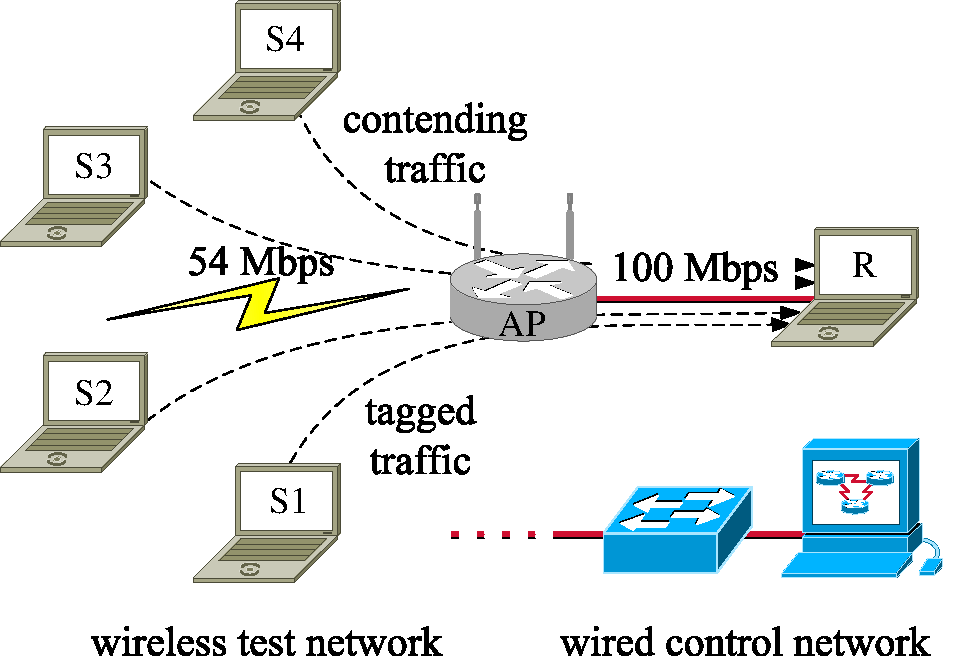
\includegraphics[width=0.5\textwidth]{gfx/examples/setup}
 \caption{Dies ist eine einfache Grafik}
 \label{fig:chapter03:setup}
\end{figure}

Aenean blandit neque eget nunc euismod ac dignissim enim euismod. Nullam semper, orci vitae elementum pretium, est lorem sodales justo, id lobortis nunc felis et justo. Cras tortor orci, rhoncus a commodo quis, aliquam eu dui. Donec pulvinar, arcu ornare consequat ultricies, purus dui accumsan massa, id auctor magna justo nec risus. Nulla bibendum, est nec ornare venenatis, lacus diam pretium augue, sed convallis orci sapien vitae lectus. In blandit massa aliquam felis feugiat fringilla.

\subsection{Grafiken mit Subfloat}
\label{sec:chapter03:grafiken:subfloat}
Quisque non massa neque. In at placerat lacus. Integer urna augue, laoreet ac mattis sed, posuere ut turpis. Nunc a metus quis elit placerat ultricies vel a eros. Quisque condimentum aliquet fermentum. Integer arcu est, suscipit quis lacinia at, volutpat nec tortor. Proin feugiat tristique est eget luctus. Suspendisse porta mauris sed sapien egestas sit amet volutpat tellus ultricies. Nulla vulputate semper turpis sed blandit. Phasellus at tortor pulvinar nisi luctus gravida.

\begin{figure}[bth]
  \myfloatalign
  \subfloat[Asia personas duo.]{
     \label{fig:chapter03:subfloat:grafik1}
     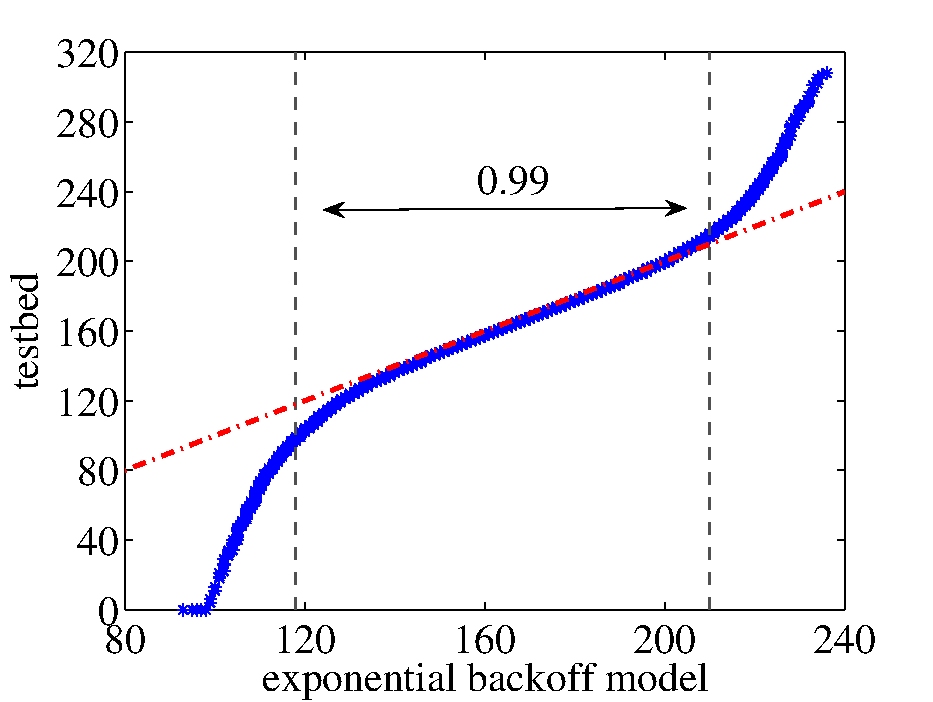
\includegraphics[width=.45\linewidth]{gfx/examples/qq-plot_gaus_vs_160}
   } \quad
   \subfloat[Pan ma signo.] {
     \label{fig:chapter03:subfloat:grafik2}
     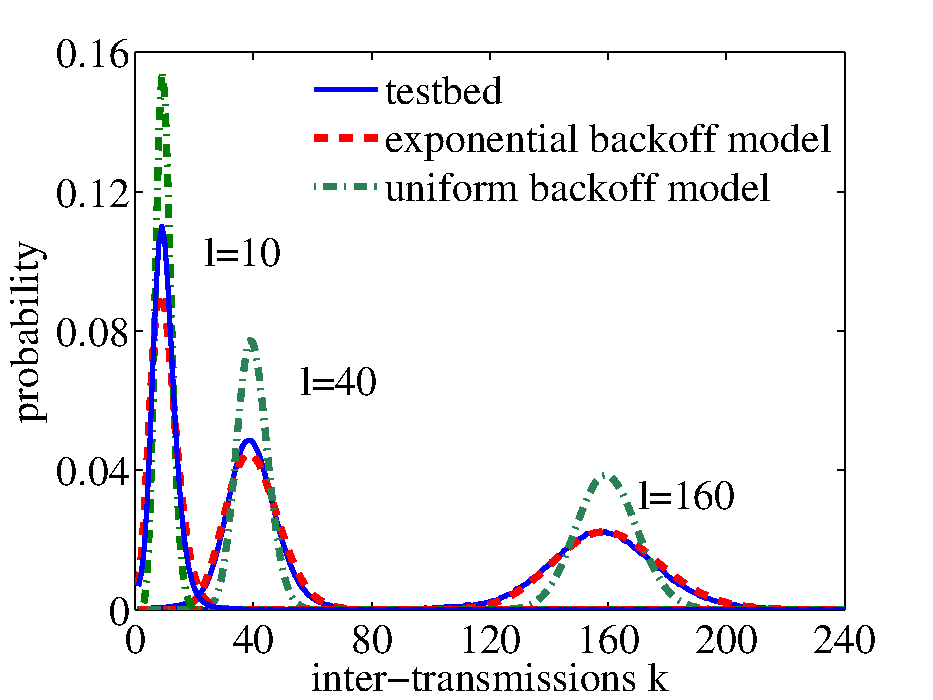
\includegraphics[width=.45\linewidth]{gfx/examples/pdf_gaus_vs_uni_vs_10_40_160}
   } \\
   \subfloat[Methodicamente o uno.]{
     \label{fig:chapter03:subfloat:grafik3}
     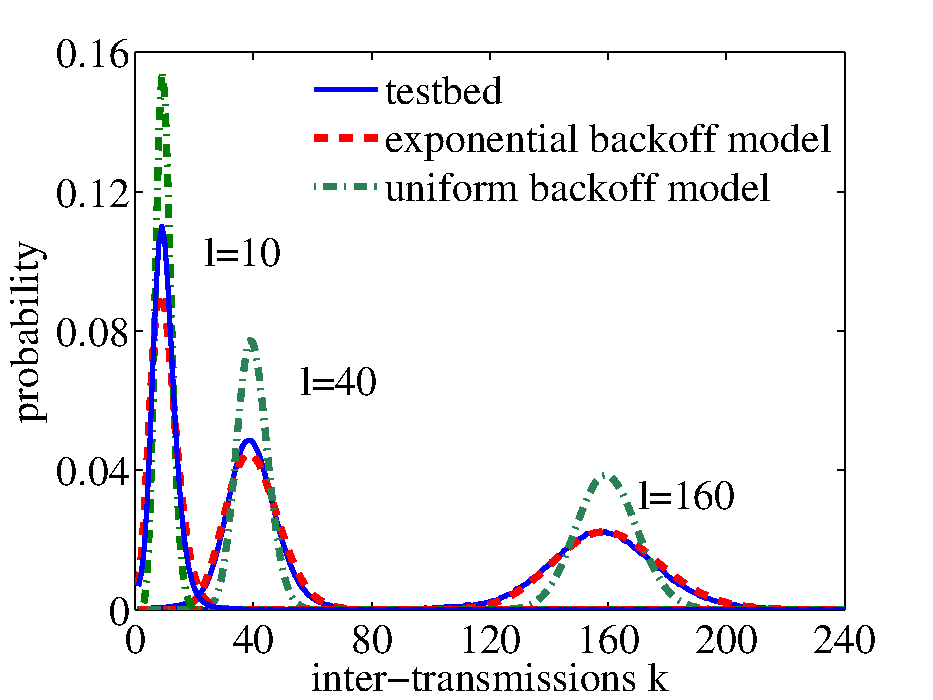
\includegraphics[width=.45\linewidth]{gfx/examples/pdf_gaus_vs_uni_vs_10_40_160}
   } \quad
   \subfloat[Titulo debitas.]{
     \label{fig:chapter03:subfloat:grafik4}
     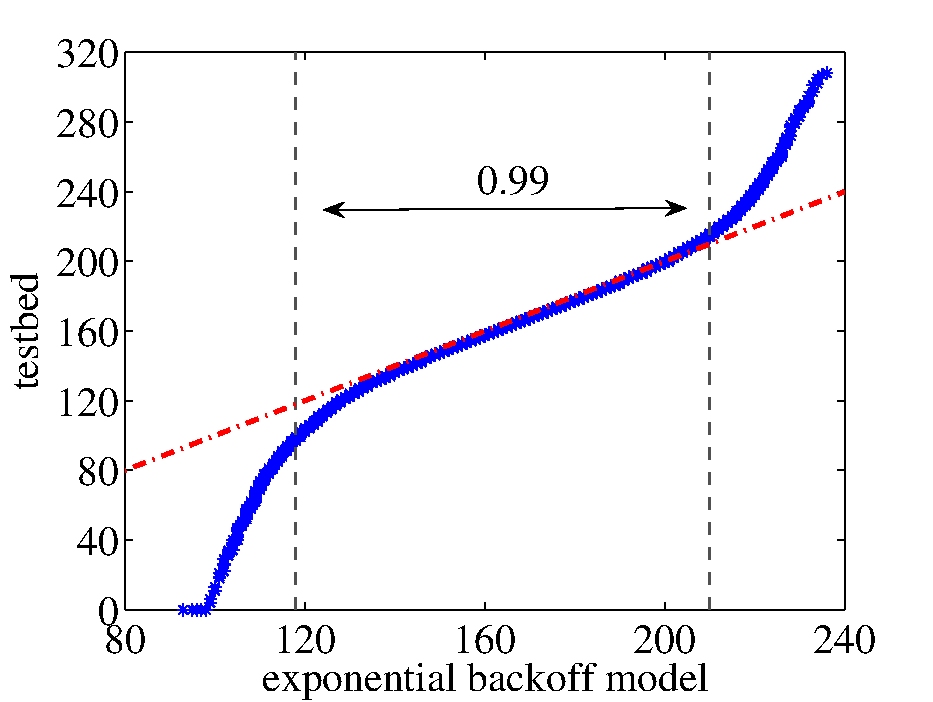
\includegraphics[width=.45\linewidth]{gfx/examples/qq-plot_gaus_vs_160}
   }
   \caption[Subfloat - Figure]{Mit Subfloat lassen sich mehrere Grafiken neben- und untereinander darstellen. Jeder Figure kann dabei mit einem eigenen Text versehen werden.}
   \label{fig:chapter03:subfloat}
\end{figure}


\subsection{Grafiken mit Minipage}
\label{sec:chapter03:grafiken:minipage}
Donec gravida consequat arcu, et mollis tortor posuere vitae. Sed pharetra turpis a ante commodo accumsan. Suspendisse leo nulla, accumsan sit amet dapibus in, posuere eget turpis. Vivamus enim sapien, porta id placerat eget, laoreet sed massa. Class aptent taciti sociosqu ad litora torquent per conubia nostra, per inceptos himenaeos.

\begin{figure}[htbp]
  \centering
  \begin{minipage}[b]{5 cm}
    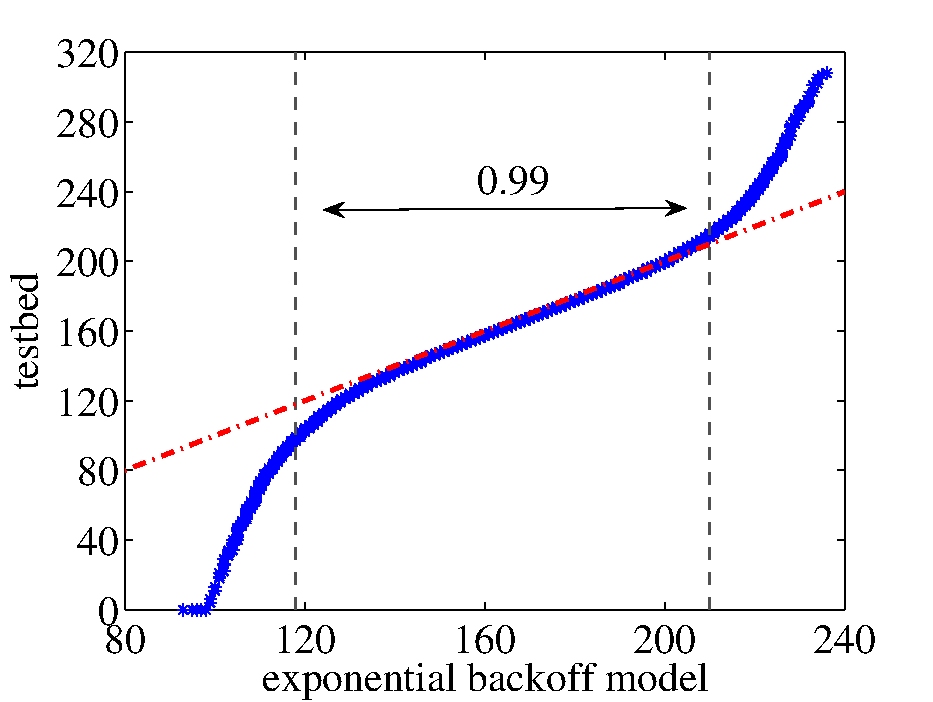
\includegraphics[width=\linewidth]{gfx/examples/qq-plot_gaus_vs_160} 
    \caption{Minipage-Grafik Nummero uno}
    \label{fig:chapter03:minipage:grafik1}
  \end{minipage}
  \begin{minipage}[b]{5 cm}
    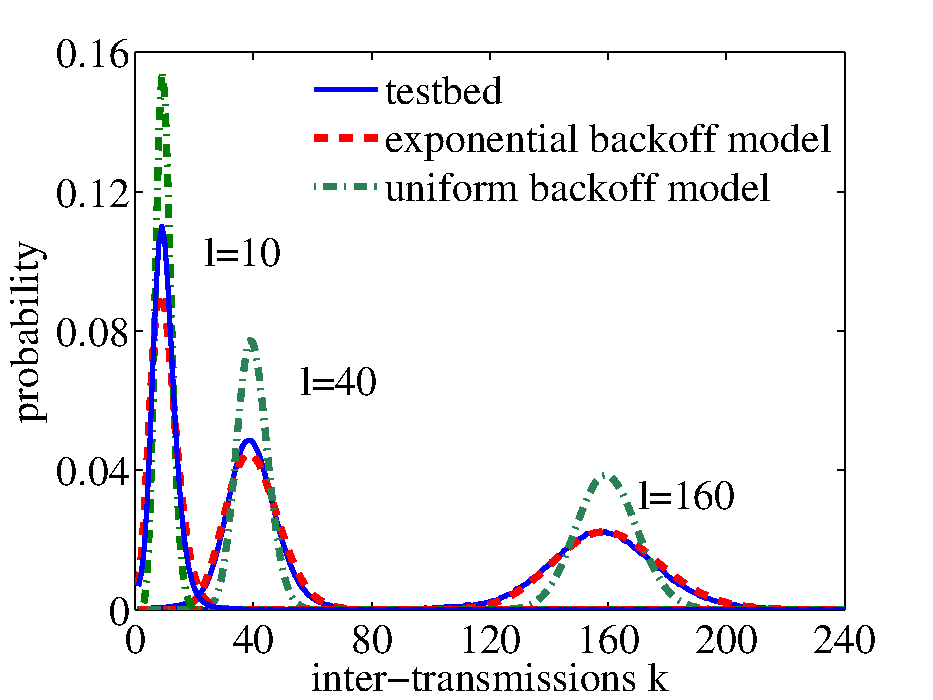
\includegraphics[width=\linewidth]{gfx/examples/pdf_gaus_vs_uni_vs_10_40_160}  
    \caption{Minipage-Grafik Nummer zwei}
    \label{fig:chapter03:minipage:grafik2}
  \end{minipage}
\end{figure}

In vitae est eget velit mattis lobortis. In hac habitasse platea dictumst. Quisque aliquam quam et justo pellentesque ullamcorper. Curabitur elementum mattis leo facilisis tincidunt. Fusce posuere viverra ultricies. Cras eget velit et ipsum gravida imperdiet et hendrerit orci.

Maecenas fringilla viverra urna ut egestas. Nulla sagittis molestie libero eget luctus. Nulla non odio sit amet magna vehicula tincidunt. Nulla accumsan ornare placerat. In posuere scelerisque quam, sed posuere urna eleifend quis. Pellentesque sed quam quis dui vulputate convallis ut ac diam. In hac habitasse platea dictumst. Donec molestie auctor dapibus. Vivamus in erat risus, ut aliquet diam. Duis vel velit ante, id ullamcorper turpis. Lorem ipsum dolor sit amet, consectetur adipiscing elit. In accumsan ornare tellus a porttitor. Etiam facilisis dui et sem eleifend id luctus nisl scelerisque. Aenean quis commodo libero. Nulla quis semper dolor. 

%
% Section: Tabellen 
%
\section{Tabellen}
\label{sec:chapter03:tabellen}
Sed lobortis vestibulum euismod. Vivamus vestibulum gravida nisi vitae condimentum. Nullam nec lacus nibh. Phasellus arcu magna, varius eget viverra a, elementum eu dolor. Aliquam erat volutpat. Sed nibh leo, vestibulum quis lacinia in, vestibulum sollicitudin nulla. In iaculis, purus in imperdiet sagittis, tortor diam pellentesque lectus, eget faucibus ante elit at tortor.

%
% Section: Listings 
%
\section{Listings}
\label{sec:chapter03:listings}
Aliquam ut pretium lectus. Curabitur in eros et sapien aliquet luctus ut sit amet eros. Proin et libero non mi venenatis aliquet at sed lorem. Ut sed enim mi, id viverra eros. Cras metus ante, placerat id commodo at, molestie non libero. Aenean eu risus erat, vel consequat metus. Sed malesuada metus sit amet nisl viverra hendrerit.


%
% Section: Equations
%
\section{Equations}
\label{sec:chapter03:equations}
Pellentesque sed quam quis dui vulputate convallis ut ac diam. In hac habitasse platea dictumst. Donec molestie auctor dapibus. Vivamus in erat risus, ut aliquet diam. Duis vel velit ante, id ullamcorper turpis.
%
\begin{equation}
 U = R * I
\end{equation}

Lorem ipsum dolor sit amet, consectetur adipiscing elit. In accumsan ornare tellus a porttitor. Etiam facilisis dui et sem eleifend id luctus nisl scelerisque. Aenean quis commodo libero. Nulla quis semper dolor.
%
\begin{equation}
 I = \frac{U}{R} 
\end{equation}

In the following we use probability theory to derive closed-form expressions for the fairness that is achieved among $M$ contending stations. We tag station $M$ and denote $K_i$ the inter-transmissions of station $i = 1 \dots M-1$ and let $K = \sum_{i=1}^{M-1} K_i$. The conditional probability $P[K\!=\!k|l]$ can be defined for $M \ge 2$ as
%
\begin{equation}
\mathsf{P}[K\!=\!k|l] = \mathsf{P} \Biggl[\sum_{i=1}^{M-1} K_i = k \Big| l \Biggr]
\label{eq:chapter03:exactpmf}
\end{equation}
%
where the random variables $K_i$ are the integers that satisfy
%
\begin{equation*}
\sum_{j=1}^{K_i} b_i(j) \le \sum_{j=1}^{l} b_M(j) \;\;\; \textmd{and} \;\;\; \sum_{j=1}^{K_i+1} b_i(j) > \sum_{j=1}^{l} b_M(j) .
\end{equation*}


%
% Section: Theorem and Proof
%
\section{Theorem and Proof}
\label{sec:chapter03:theorem}
We use the central limit theorem to derive the long-term fairness. In the sequel, we denote normal random variables $N(\mu,\sigma^2)$ where $\mu$ is the mean and $\sigma^2$ the variance.
%
\begin{Theorem}[Gaussian approximation]
\label{th:chapter03:twostationsgaussian}
%
Let the $b_i(j)$ be i.i.d. random variables with mean $\mu$ and variance $\sigma^2$ and let $M=2$. For $k,l \gg 1$ (\ref{eq:chapter03:exactpmf}) is approximately Gaussian where
%
\begin{equation*}
\mathsf{P}[K \!\le\! k|l] \approx \mathsf{P}\biggl[ N(0,1) \le \frac{\mu\,(k-l)}{\sigma\,\sqrt{k+l}} \biggr] .
\end{equation*}
%
\end{Theorem}
%
\begin{proof}
%
For $M=2$ we have from (\ref{eq:chapter03:exactpmf}) that
%
\begin{equation*}
\mathsf{P}[K \!<\! k|l] = \mathsf{P} \Biggl[\, \sum_{j=1}^k b_1(j) > \sum_{j=1}^l b_2(j) \Biggr]
\end{equation*}
%
and after expansion and some normalization this equals
%
\begin{equation*}
= \mathsf{P}\Biggl[ \frac{\sum_{j=1}^{l}b_2(j) - l\mu}{\sigma\sqrt{l}} - \frac{\sum_{j=1}^{k}b_1(j) - k\mu}{\sigma\sqrt{l}} < \frac{\mu(k-l)}{\sigma\sqrt{l}} \Biggr].
\end{equation*}
%
Using the central limit theorem it follows that
%
\begin{equation*}
\mathsf{P}[K \!<\! k|l] \approx \mathsf{P} \biggl[ N(0,1) - N \biggl(0,\frac{k}{l}\biggr) < \frac{\mu(k-l)}{\sigma\sqrt{l}} \biggr] .
\end{equation*}
%
Since the normal distribution with zero mean is symmetric we can replace the subtraction of $N(0,k/l)$ by addition. Furthermore, the sum of two normal random variables $N(\mu_1, \sigma_1^2)$ and $N(\mu_2, \sigma_2^2)$ is normal with $N(\mu_1+\mu_2, \sigma_1^2+ \sigma_2^2)$ such that
%
\begin{equation*}
\mathsf{P}[K \!<\! k|l] \approx \mathsf{P} \biggl[ N\biggl(0,\frac{k+l}{l}\biggr) < \frac{\mu(k-l)}{\sigma\sqrt{l}} \biggr] .
\end{equation*}
%
Finally, we use that if $X$ is $N(a\mu,a^2\sigma^2)$ then $Y = X/a$ is $N(\mu,\sigma^2)$ with $a^2 = (k+l)/l$ to standardize the result.
%
\end{proof}

Th. \ref{th:chapter03:twostationsgaussian} assumes i.i.d. random countdown values. It does, however, not make any assumption about their distribution.

\chapter{Introduction}
\label{ch01:intro}

% \section{Motivation}
% \label{ch01:intro:motivation}
With the ever-present and rapid technological progress, it remains important to keep in mind that legacy systems do not simply disappear with every new advancement. Legacy systems like Adabas, a 1971 non-relational database, remain essential for enterprise applications requiring high-volume transaction processing. However, the use of systems like Adabas represent challenges in integrating them with modern systems and use cases, especially since Adabas programs are mostly written using the proprietary Natural language. This increases the difficulty and cost of maintance \cite{ibm_redpaper_key}. In some enterprise cases, a relational database is preferred on top of the existing Adabas hosted on mainframe. The benefits can include the flexibility and widespread use of SQL queries, triggers, referential constraints, and a more simplified integration with modern systems \cite{ibm_redpaper_key}.

To modernize Adabas, the \ac{ART} for Adabas on z/OS was developed for the replication of Adabas changes to other systems. A proprietary product of Software GmbH, it supports the replication to various supported systems, called \textit{targets}. The majority of supported targets are relational databases such as MySQL, PostgreSQL, and DB2. \ac{ART} also supports replicating to Adabas on \ac{LUW} or to Kafka.

However, the Target Adapter has some drawbacks, which have been noted both by clients and developers. These include performance issues when replicating to relational databases and a lack of parallelization support, which can also be detrimental to performance. Recent customer demand also included replication support to Apache Kafka. While \ac{ART} has support for Kafka, the lack of parallel processing can act as a bottleneck, preventing the full use of Kafka's potential. This served as motivation for a semester project to use the existing Kafka Connect framework to write a custom source connector prototype for Kafka, which would allow replicating Adabas changes to a Kafka topic.

The project was later extended to provide a proof of concept for replication to a relational database using a Kafka-native pipeline, with Kafka's inherent parallelization and scalability capabilities \cite{peddireddy2023kafkadatalakebenefits} as its main advantage over \ac{ART}.

\section{Research Question}
\label{ch01:intro:researchquestion}
To explore in what ways a Kafka replication pipeline, despite higher complexity and multiple components, can compete with the existing \ac{ART} solution, the following research question was chosen: \textbf{"How does the performance of a Kafka Connect-based replication pipeline for Adabas on mainframe compare to the Adabas Event Replicator Target Adapter?"}. The proof of concept developed for replication to a relational database will be used for direct comparison with \ac{ART} in terms of performance, with the aim of exploring their relative strengths and weaknesses. The research hypothesis states that the Kafka Connect-based replication will outperform \ac{ART} if it takes advantage of its parallelization capabilities. If it is run as a single-thread application, then the performance will be equal or even worse, due to the higher complexity from multiple components and related latency.

\section{Thesis Structure}
\label{ch01:intro:thesisstructure}
First, the fundamentals of both Adabas-related and Kafka-related technologies relevant to this thesis are covered in Chapter \ref{ch02:fundamentals}. This includes Adabas for z/OS, the the Adabas Event Replicator, and the Event Replicator Target Adapter for the Adabas-related fundamentals. The Kafka-related fundamentals cover Apache Kafka, the Kafka Connect framework, and the schema registry. Chapter \ref{ch03:litreview} then covers the related work for the outlined technologies. The development of the Kafka-based replication solution is covered in Chapter \ref{ch04:pipelinedevelopment}, with its design, implementation, and additional considerations. The methodology of the experiment is described in Chapter \ref{ch05:methodology}, as well as the environment setup and conditions of the experiment. Afterwards, the measured performance results from the experiment are described in Chapter \ref{ch06:results}. The results are further discussed in Chapter \ref{ch07:discussion}, providing a comprehensive analysis of the results and examining the statistical significance. The effects of parallelization and other architectural considerations are also discussed. Last but not least, the key findings of the thesis and future work possibilities are summarized in Chapter \ref{ch08:conclusion}.
\chapter{Fundamentals}
\label{ch02:fundamentals}

\section{Adabas}
\label{ch02:fundamentals:adabas}
Adabas, short for \textbf{Ada}ptable Data\textbf{ba}se \textbf{S}ystem, is a high-performance transactional \ac{DBMS} first launched on a mainframe in 1971. Since then, Adabas has grown to also become available on a variety of systems, including Microsoft Windows, Linux, and other Unix-based platforms. It now includes a range of products, both for the mainframe and \ac{LUW} versions \cite{adabasconcepts}. As the thesis scope is restricted to Adabas on mainframes, the focus of the following fundamentals will be on Adabas for z/OS.

\subsection{Adabas for z/OS}
\label{ch02:fundamentals:adabas:forzos}
% important adabas terminology for understanding paper
\subsubsection{Adabas Terminology}
To understand Adabas, there are a few definitions fundamental to it that have to be addressed. As a \ac{DBMS}, Adabas can manage multiple databases. Each \textit{database} is a collection of \textit{files}, which are best compared to tables in a relational database. Each file is a "group of related \textit{records}" \cite{adabasconcepts}, which in turn are a "collection of related \textit{fields}" % that make up a complete unit of information???
\cite{adabasconcepts}. Records are comparable to a table row in a relational database, as they usually represent the entire data unit of the represented entity (for example the data of a single employee). The record fields represent the "smallest logical unit of information" \cite{adabasconcepts} and can be grouped into different denormalized data structures.

\subsubsection{Classifying Adabas}
\label{ch02:fundamentals:adabas:forzos:classifying}
% what kind of database is adabas?
Adabas is sometimes called a pre-relational database \cite{ibm_redpaper_key} due to its launch approximately around the same time (or even shortly before) the relational model. Before the relational model, the most common data models were the hierarchical (such as the IBM IMS) and network model \cite{stonebrakerwhatgoesaroundcomesaround}. Adabas is considered a "relational-like \ac{DBMS} with some network features" \cite{adabashybrid}. It has features of the network data model, including support for many-to-many relationships between fields, which are achieved with the multiple field and periodic group structures (discussed further in \ref{ch02:fundamentals:adabas:forzos:datastructures}).

Adabas also contains similar features to a relational data model, such as table-like structures, which can reference one another based on a unique identifier. In the case of Adabas files, the unique identifier is called the \ac{ISN}. Adabas supports both physical coupling of files (similarly to network models) and logical coupling of files \cite{adabasconcepts}. As opposed to the network or hierarchical data model, the coupling relationship is not hierarchical, but instead bidirectional. In the case of physical coupling, files are explicitly linked in the \textit{coupling lists} (managed by the Adabas nucleus) for both files \cite{adabashybrid}. In the case of logical coupling, files can be linked in a query by specifying the common field \cite{adabasconcepts}. % TODO: verify with matthias whether correct!

\subsubsection{The Adabas Nucleus}
% first talk about components such as ASSO, then go into the details
The Adabas nucleus is the core component of the Adabas \ac{DBMS}, containing programs that manage it and allow access to Adabas files. The nucleus uses different database components, each representing a physical disk area, for managing stored data and its retrieval. There are three main components: \textit{ASSO} (Associator), \textit{DATA} (Data Storage), and \textit{WORK} (Work area) \cite{adabasconcepts}.

ASSO is used as an organizational component, storing data structures for data retrieval from the DATA component. It contains elements such as general information about the database, the \ac{FDT} (comparable to a schema) for each file, and the coupling lists mentioned in \ref{ch02:fundamentals:adabas:forzos:classifying} for the coupling of different files in a database \cite{adabasconcepts}. The ASSO also contains \textit{inverted lists} for each file, which is a key feature of Adabas for indexing records by their logical sequence when performing search and read commands \cite{adabashybrid}. In an Adabas file, multiple fields can be labeled \textit{descriptors}. The value of such descriptor fields is then stored in the inverted list with their designated \ac{ISN}s. Thus the list is inverted, as it is ordered by the descriptor values \cite{adabasconcepts}. The ASSO also contains an \textit{address converter} for determining the physical location of each record, called the \ac{RABN}, based on its \ac{ISN}. This allows for physical data independence, as the physical record data can be moved around based on available free space in the DATA component without having to modify the inverted lists \cite{adabashybrid}. 

The DATA component stores the actual record data in a compressed format. It is split up into blocks which are identified by the \ac{RABN}. Each block can contain multiple records depending on their size, as well as some reserved space as padding to allow for the growth of records. Adabas also allows for the physical migration of records in case of growth that the current block cannot support, allowing the database to remain functional and optimized even in case of a growing number (or size) of records \cite{adabasconcepts}.

The WORK component acts as an area for storing information related to transaction routines, two-phase commit processing, and the results of search commands. There exist also further components for specific Adabas utilities, including optional logs. The \ac{CLOG}, for example, is used for keeping information on issued Adabas commands in order to establish an audit trail, while the \ac{PLOG} is used to capture data change in the database, in case there is need for recovery \cite{adabasconcepts}.

\subsubsection{Adabas Data Structures}
\label{ch02:fundamentals:adabas:forzos:datastructures}
% adabas data structures
All of the fields in a file are specified in the \ac{FDT}, which is then used to create the file. Unlike in relational databases, where column order is irrelevant, the order of fields defined in the \ac{FDT} is important and can influence the efficiency of their retrieval \cite{storr1994effizienter}.

"Flat" Adabas fields can have different formats, including packed and unpacked decimals, alphanumeric, and binary. Adabas also has multiple denormalized data structures into which fields can be grouped. It supports groups, multiple fields (MU), and periodic groups (PE), as well as multiple fields in periodic groups \cite{aebi1996reengineering}. A group, as the name suggests, is a grouping of multiple fields under one "parent" name. A group can contain multiple levels (up to 6 levels of nested groups) \cite{storr1994effizienter}. It is recommended to group fields if they are often accessed and are ordered together, allowing faster retrieval by group name \cite{adabasconcepts}. This again highlights the need for fields to be ordered properly in an \ac{FDT}. Multiple fields represent an array of the "flat" Adabas fields, while a periodic group represents multiple instances of a group of fields (an array of a group). Figure \ref{fig:fundamentals:datastructure} shows an example record (without its \ac{ISN}) containing different field types:
\begin{itemize}
    \item Flat fields PERSONNEL\_ID, MARSTAT, SEX
    \item Group field FULLNAME with level 2 sub-fields FIRST\_NAME, NAME, MIDDLE\_NAME
    \item Periodic group field of two occurrences with fields CURRCODE, SALARY, and multiple field BONUS (containing 3 MU occurrences in the first PE occurence, and 2 MU occurrences in the second PE occurrence)
    \item Multiple field LANG with 3 occurrences
\end{itemize}

\begin{figure}[htbp]
 \centering
 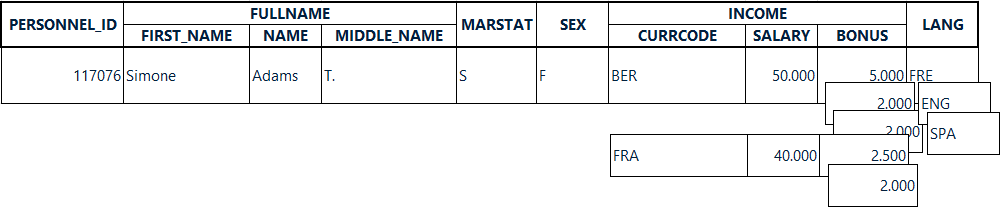
\includegraphics[width=1\textwidth]{chapters/images/datastructures.png}
 \caption{Example structure of a record containing various Adabas data structures}
 \label{fig:fundamentals:datastructure}
\end{figure}

\subsubsection{Adabas Transactions}
\label{ch02:fundamentals:adabas:forzos:transactions}
Adabas operates with so-called \textit{logical transactions}: the transaction contains a user-defined \ac{UOW} that must be committed and processed as an atomary \ac{UOW} with the all-or-nothing principle. A transaction has to end either with an \ac{ET} command (in case of success) or with a \ac{BT} command (in case of an error or other issue). If the \ac{BT} command is issued, a rollback is performed of all the updates within that transaction \cite{adabasconcepts}.

% The \ac{REPTOR} (see \ref{ch02:fundamentals:adabas:reptor}) identifies each transaction with its transaction commit time and sequence number (which is relative, as it is always reset when the \ac{REPTOR} restarts). - include in reptor fundamentals
\subsection{Adabas Event Replicator}
\label{ch02:fundamentals:adabas:reptor}
The \ac{REPTOR} was developed by Software GmbH as a replication solution for capturing changes in Adabas files. It is made up of multiple components, also hosted on the mainframe, which facilitate the replication of any record modifications processed by the Adabas nucleus \cite{storr2011reptor}.

\begin{figure}[htbp]
 \centering
 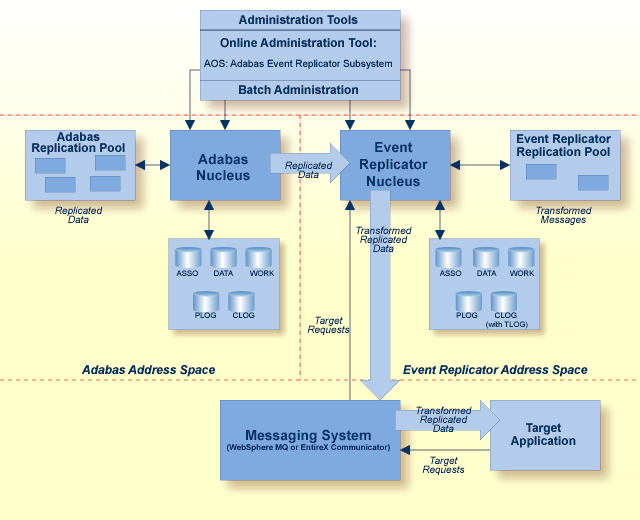
\includegraphics[width=0.8\textwidth]{chapters/images/reptor_architecture.png}
 \caption{Adabas and Event Replicator Components \cite{reptorconcepts}}
 \label{fig:fundamentals:reptorarchitecture}
\end{figure}

As shown in Figure \ref{fig:fundamentals:reptorarchitecture}, any record changes processed by the Adabas nucleus are replicated and stored in the Adabas replication pool until a transaction commit occurs. After the \ac{ET} command, the committed data is copied from the Adabas replication pool, transformed, and saved to the \ac{REPTOR} replication pool. After the transformed transaction messages have been processed by a pre-defined set of rules (called a \textit{subscription}), they are sent to a messaging system\footnote{There are currently two messaging systems supported: the IBM MQ or the EntireX Broker.}. After the replication process is completed and successfully sent to the messaging system, the replicated transaction data is deleted from both replication pools \cite{reptorconcepts}. The target application consuming the message queue can also send requests to the \ac{REPTOR} nucleus through the messaging system, such as requests for status messages. If the messaging system is unavailable or the \ac{REPTOR} replication pool starts to overflow, the overflowing transactions can be written to the \ac{SLOG} file to prevent their loss \cite{storr2011reptor}. The \ac{REPTOR} supports two formats for replicated messages: XML and binary \cite{artconcepts}.

\ac{REPTOR} messages can be classified into four different event types: Delete, Insert, \ac{IS}, and Update. The \ac{IS} event is an event in which the entire current state of the Adabas file is sent \cite{reptorprogrammersref}. This is necessary, for example, when populating the target database for the first time. The \ac{IS} event can be transmitted to the target application using the same messaging system as the other \ac{REPTOR} events. However, there also exists an Adabas utility called ADARIS, which allows the entire \ac{IS} to be split up and written to one or more sequential files. These can then be imported and processed by the target application \cite{reptorconcepts}. This can be quite beneficial, as \ac{IS} volumes can get quite large in enterprise systems with over a million records.

\subsubsection{EntireX Broker}
\label{ch02:fundamentals:adabas:entirex}
The message queue covered in this thesis is the EntireX Broker, as it was already being used internally for development. The EntireX Broker acts as message-oriented middleware, allowing reliable communication with high performance and availability \cite{entirexbrokerintro}. It supports transactional integrity by using units of work\footnote{Not to be confused with the transactional \ac{UOW} from \ref{ch02:fundamentals:adabas:forzos:transactions}.} to group together messages, which are then treated by the Broker as an atomary unit. Message delivery is guaranteed by the receiver application, which must send a COMMIT acknowledgement for each \ac{UOW} received. If a client receives the \ac{UOW} and processes it but does not send a COMMIT message to the Broker, that specific \ac{UOW} can be re-delivered to the message queue, marked as timed out, or processed in some other way based on the broker configuration \cite{entirexbrokeradmin}. This is useful in the case that a client application receives the messages but fails or crashes before it is able to process them fully, preventing a COMMIT message from being sent. In that case, it would be necessary for all the messages within the unprocessed \ac{UOW} to be re-processed by the client application once it is running again.

\subsection{Event Replicator Target Adapter}
\label{ch02:fundamentals:adabas:art}
The Event Replicator Target Adapter (\ac{ART}) is another Software GmbH product that allows the transformation of replicated data into a specified format, allowing the transformed data to be applied to a target application, such as a relational database \cite{artconcepts}. Although \ac{ART} was initially created for various relational databases as targets, it supports any custom target which was developed using the publicly available source code\footnote{\url{https://github.com/SoftwareAG/adabas-user-targets}}. This can include a custom target solution for a data warehouse or a custom Kafka producer.

\ac{ART} can be installed using the Software GmbH installer, which also provides the Administration tool for a graphical user interface and a Replication Monitoring tool to visualize the status of the \ac{REPTOR} \cite{artconcepts}. However, it can also run headless as a Dockerized instance, with the XML configuration files added manually.

\subsubsection{Schema Transformation}
\label{ch02:fundamentals:adabas:art:schematransformation}
To allow Adabas records to be inserted into a relational database, they first have to be flattened and normalized if they contain any of the aforementioned data structures from \ref{ch02:fundamentals:adabas:forzos:datastructures}. \ac{ART} has a Data Mapping Tool for defining a custom relational schema for the target. There also exists a default transformation \cite{artconcepts}. The following data structures are affected in the default transformation \cite{artconcepts}:
\begin{description}
\item [Group fields]
Group fields are flattened by adding the child fields directly to the root table. In the case of the group field FULLNAME from Figure \ref{fig:fundamentals:datastructure}, the table will contain the fields FIRST\_NAME, NAME, and MIDDLE\_NAME.
\item [Multiple fields]
Each MU field is mapped to a separate relational table, where each value is represented as a separate row with the possibility of tracking the MU index\footnote{An index, or occurrence, indicates the position of the value in the repeating MU or PE field.} as a separate column. The LANG field in Figure \ref{ch02:fundamentals:adabas:forzos:datastructures} is an MU field with three occurrences. Listing \ref{lst:bonusmuquery}  shows how the MU field would be structured in the table. The foreign key constraint is inherited from the root table primary key(s). 
\item[Periodic groups]
Each PE group is also mapped to a separate relational table. Each sub-field in the periodic group is represented by a column in the table. An additional index field is created, composed from the \ac{ISN} and PE field index, which serves as the primary key. The foreign key constraint that references the root table is on the \ac{ISN} field. An example PE field can be seen in listing \ref{lst:bonusmuquery}.

In the case of an MU field in a PE group, a separate table is created with the same logic as a typical MU table, except that an IX2 field is used instead of the IX field to show its nested nature. The aforementioned composed index field is also added to the new MU table with a foreign key constraint referencing the parent PE table. An example MU field in a PE group can be seen in Listing \ref{lst:bonusmupequery}.
% TODO: pk and fk fields of the index, reference listing
\end{description}

\begin{lstlisting}[frame=tb,caption={Query result of the MU field LANG in the relational table EMPL\_LANG},label=lst:bonusmuquery]
 ISN | LANG | LANG_IX
-----+------+---------
   1 | FRE  |       1
   1 | ENG  |       2
   1 | SPA  |       3
\end{lstlisting}

\begin{lstlisting}[frame=tb,caption={Query result of the PE field INCOME in the relational table EMPL\_INCOME},label=lst:incomepequery]
  ISN   | INCOME_INDEX | ISN_INCOME_INDEX | CURRCODE | SALARY
--------+--------------+------------------+----------+--------
      1 |            1 |      1_1         | BER      |  50000
      1 |            2 |      1_2         | FRA      |  40000
\end{lstlisting}
\newpage
\begin{lstlisting}[frame=tb,caption={Query result of the MU field BONUS in the PE field INCOME in the relational table EMPL\_INCOME\_BONUS},label=lst:bonusmupequery]
 ISN_INCOME_INDEX | BONUS | BONUS_IX2
------------------+-------+-----------
 1_1              |  5000 |         1
 1_1              |  2000 |         2
 1_1              |  2000 |         3
 1_2              |  2500 |         1
 1_2              |  2000 |         2
\end{lstlisting}


\subsubsection{Drawbacks of the Target Adapter}
\label{ch02:fundamentals:adabas:art:limitations}
There have been some performance concerns noted both by clients and developers when using \ac{ART} to replicate to a relational database. Possible causes could be the fact that \ac{ART} for Adabas on mainframe only supports messages in XML format, which can negatively impact performance \cite{nicola2003xml}. Another cause is speculated to be the lack of parallelism when replicating to relational databases. The only parallel processing that is supported by \ac{ART} is when loading the \ac{IS} using multiple ADARIS-generated files. This can be achieved by running multiple instances of \ac{ART}, where each instance processes one of the generated ADARIS files.

\section{The Kafka Ecosystem}
\label{ch02:fundamentals:apachekafkaandkafkaconnect}

\subsection{Apache Kafka}
\label{ch02:fundamentals:apachekafkaandkafkaconnect:apachekafka}
Apache Kafka is a distributed event streaming platform developed by LinkedIn and currently managed by the Apache Foundation, offering high-throughput and fault-tolerant data processing. A behemoth of streaming possibilities, it runs as a cluster of one or more machines called \textit{brokers}. They organize incoming messages (also called events by Kafka) in \textit{topics}, which can be asynchronously published to with \textit{producers} and consumed from by \textit{consumers} \cite{peddireddystreamliningprocessingkafka}. To facilitate scalability and distributed processing, a topic can be divided into multiple \textit{partitions}. Message order is only guaranteed for a single partition, so that if two messages are added in a consequent order to two different partitions, they will not necessarily be consumed in the same order. Messages are organized by a sequential \textit{offset} number in each partition \cite{thein2014apache}.

There are different strategies for determining which partition a message is assigned to. The default strategy involves hashing the message key to map it to a partition. If the key is null, either the "sticky partition" strategy is used (where messages get produced to one partition until a certain batch size is achieved) or the round-robin strategy. Kafka also supports writing custom partitioners to implement a specialized partitioning strategy  \cite{kafkadocumentation}.

Partitions can be stored on different brokers running in the same cluster, so that client applications can consume from and produce to different brokers, improving load balancing and scalability. Partitions can also be replicated to different brokers (the number of replicas is determined by the \textit{replication factor} configuration), improving Kafka's fault tolerance \cite{thein2014apache}. Each partition gets assigned a broker leader, with that broker then being responsible for the reads and writes to that partition. The rest of the brokers act as "followers" for that partition and have the ability replicate it, depending on the cluster configuration \cite{petrescukafkaraft}. These brokers then maintain the so-called \ac{ISR} of the partition. This mechanism guarantees message consistency and fault tolerance for the consumer, as a message is only ever truly considered committed (and available to a consumer) if the specified number of \ac{ISR} are synchronized with the leader partition \cite{kafkadocumentation}.

Kafka provides three possible message delivery guarantees, using the message offset to track a consumer's position in a partition: at most once, the default at least once, and exactly once \cite{kafkadocumentation}. Kafka uses the notion of \textit{consumer groups}, where the message offset position is tracked for each group instead of the individual consumer. If there are multiple consumers in one consumer group, each message is delivered to only one of them \cite{kreps2011kafka}.

Older versions of Kafka rely on Zookeeper, a separate service mainly used for organizing brokers and consumers, keeping track of consumer groups and their progress, and rebalancing consumers in case of consumer load or broker number change \cite{kreps2011kafka}. It facilitates leader election in the Kafka cluster, so that a single controller can be chosen among the brokers to make cluster-relevant decisions. One such decision is assigning partition leader roles. However, as of Kafka version 3.5, Zookeeper is marked as deprecated and planned for removal \cite{kafkadocumentation}. Instead, Kafka now supports running in KRaft mode, based on the Raft concensus algorithm \cite{ongaroraft2014search}. In KRaft mode, Kafka nodes can act as brokers, controllers, or both, removing the need for Zookeeper. The Kafka nodes assigned the controller role participate in a quorum to elect a controller leader \cite{kafkadocumentation}.

It is important to note that Kafka is not intended to be used as a permanent storage for events. Instead, it has a configurable retention period (specified in time and/or byte size), after which messages are deleted from the brokers. This allows for a certain "grace period", in case older offsets need to be consumed again, without keeping old and unnecessary data for too long \cite{kreps2011kafka}.

\subsection{Kafka Connect}
\label{ch02:fundamentals:apachekafkaandkafkaconnect:kafkaconnect}
Kafka Connect is an open-source framework developed for Apache Kafka to allow for reliable and scalable data integration between Kafka and external systems such as databases. The Apache Foundation offers publicly available \ac{APIs} for implementing source connectors (to produce data to Kafka) and sink connectors (to consume from Kafka and write to external systems) \cite{kafkadocumentation}. Some companies such as Confluent provide already existing connectors, such as the \ac{JDBC} source and sink connectors\footnote{\url{https://github.com/confluentinc/kafka-connect-jdbc}}.

While it is possible to not use Kafka Connect and instead write producers as part of the source system to capture any changes, tests performed by \cite{srijithkafkaconnectperformance} have shown that the traditional publish-subscribe model can perform worse than a Kafka Connect pipeline. Furthermore, \cite{maison2023kafkaconnect} identified the number of threads reserved for producer operations in the source system as a possible performance bottleneck. This is improved with Kafka connectors, which can be scaled independently of the source system, showing positive performance results in both papers.

Kafka Connect has two modes: standalone and distributed. In standalone mode, the Kafka Connect setup consists of a single host node (\textit{worker}) that can run multiple tasks. The task is the component that actually does the data processing and transfer in the connector, and is assigned the work by the connector \cite{kafkadocumentation}. In distributed mode, the setup consists of multiple workers running as a Connect cluster. The workers are able to distribute the tasks between themselves for a more equal workload, as well as take over tasks from a crashed or unavailable worker \cite{maison2023kafkaconnect}. It is also possible to run multiple connectors (for example source and sink) in the same Connect cluster (see Figure \ref{fig:fundamentals:kafkaconnectexample}). When running in distributed mode, the offset and configuration data necessary to run the connectors is stored in internal Kafka topics \cite{kafkadocumentation}.

\begin{figure}[htbp]
 \centering
 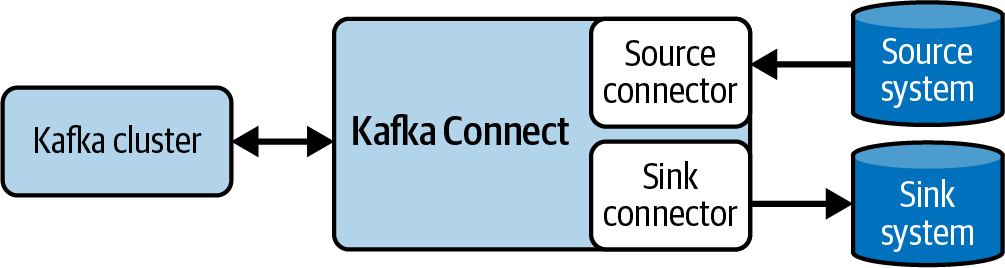
\includegraphics[width=0.6\textwidth]{chapters/images/kafkaconnectexample.png}
 \caption{Visualization of Kafka Connect with Sink and Source Connector \cite{maison2023kafkaconnect}}
 \label{fig:fundamentals:kafkaconnectexample}
\end{figure}

The number of tasks run by each connector is determined by the \textit{tasks.max} configuration. The number of active tasks in source connectors is also typically constrained by the number of source partitions, if the source is partitioned at all. Not to be confused with topic partitions, source partitions are used for splitting up the source into logical groups. For example, partitioning the source can mean to assign specific table rows to each source partition. Each source partition can be assigned a single task to process it (meanwhile, a task can process multiple source partitions). This allows the source connector to parallelize the processing of the source. A similar concept applied to sink connectors, where the number of active tasks is constrained by the number of available topic partitions \cite{maison2023kafkaconnect}.

Figure \ref{fig:fundamentals:kafkaconnectarchitecture} shows the possible architecture of a source connector running in distributed mode with two Connect workers. There are 4 tasks running and 5 source partitions, so the first task gets assigned two of the source partitions. As per the default partitioning strategy, each event processed by the task is assigned a message key before it gets produced to Kafka. This key is then used to determine the topic partition that the message is assigned to.

\begin{figure}[htbp]
 \centering
 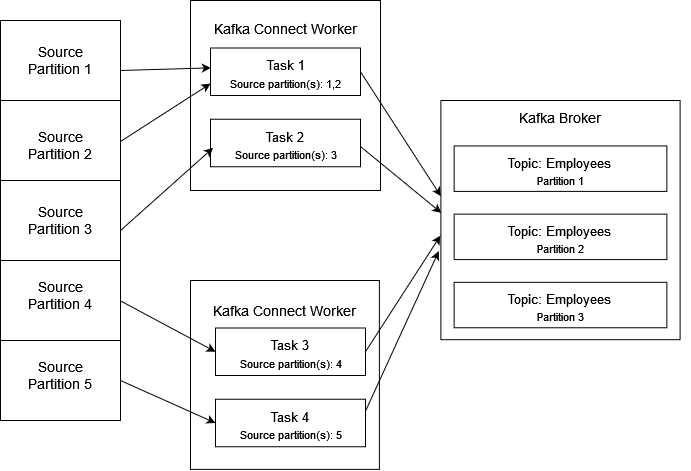
\includegraphics[width=1\textwidth]{chapters/images/kafka connect architecture enlarged.drawio.png}
 \caption{Example Architecture of a Kafka Source Connector in Distributed Mode}
 \label{fig:fundamentals:kafkaconnectarchitecture}
\end{figure}

% \subsection{Transactionality in Kafka}

\subsection{Schema Registry}
The schema registry is a component that is not native to Apache Kafka, but is a third-party addition. It is run as a separate service, and allows for the creation, management, and evolution tracking of message schemas. With it, the producer and consumer can establish a "data contract", so that events produced to Kafka can be deserialized and read properly \cite{kreps2011kafka}. This is especially useful as Kafka supports different serialization formats such as JSON, Protobuf, and Avro \cite{kafkadocumentation}.
% Although the same can be accomplished without the registry by sending the message schema with every event, the message size increase and resulting performance impact should be taken into account.

% \section{Database Replication}
% \label{ch02:fundamentals:databasereplication}

% \subsection{Relational Databases}
% \label{ch02:fundamentals:databasereplication:relationaldatabases}

% \subsection{Schema Transformation}
% \label{ch02:fundamentals:databasereplication:schematransformation}
\chapter{Related Work}
\label{ch03:litreview}
Unfortunately, there is no recent research regarding the replication of Adabas to relational (or other) databases. While there is research regarding the replication of modern NoSQL databases such as MongoDB to relational databases \cite{aftabnosqletltordbms}, the modern NoSQL differs too much from Adabas for it to truly be comparable. Instead, the related work to specific technologies relevant to this thesis are discussed.

\section{Adabas}
\label{ch03:litreview:adabas}
The state of research on Adabas is scarce and, for the most part, outdated. One such example is the research on creating a multi-database system with heterogeneous \ac{DBMS}s based on \ac{CORBA} \cite{ozhan1996making}. This system included Adabas and Oracle7, a relational \ac{DBMS}. Almost 30 years since that publication, \ac{CORBA} is considered obsolete \cite{fallofcorba}.

Another interesting, albeit outdated, paper documents the integration of Adabas with modern systems using the \ac{SOA} approach \cite{koschelmainframemodernization}. This paper explores the creation of a web service for interacting with Adabas using Natural programs. The web service used the \ac{SOAP} to communicate with the EntireX Broker, allowing it to execute Natural programs with \ac{RPC}. However, just as \ac{CORBA}, \ac{SOAP} is now considered an outdated technology \cite{soapoutdated}.

\section{Apache Kafka}
Several studies have explored the capabilities of Apache Kafka in different use cases. For instance, a research paper released by the co-creators of Kafka outlines how Kafka's design makes it more efficient and performant in comparison to other existing messaging systems such as Apache ActiveMQ \cite{kreps2011kafka}. The paper also discusses Kafka's performance guarantees and limitations when the Kafka cluster encounters extremely high throughput. It provides a description of how Kafka is used at LinkedIn, and an experimental study where the performance of Kafka is compared with Apache ActiveMQ and RabbitMQ. Another paper provides an overview of a possible architecture for implementing Kafka in a financial enterprise system for real-time data processing, reporting and alerting \cite{peddireddystreamliningprocessingkafka}. This paper also mentions using Kafka Connect (see also \ref{ch03:litreview:kafkaconnect}) for ingesting from different sources, providing case studies where Kafka has been implemented for real-time data processing. A further paper proposes a streaming system based on Kafka to replace a current event notification system based on ActiveMQ in a financial enterprise system \cite{sanjanaenterprise}. It also discusses using Kafka Streams, a built-in API for stream processing, for real-time transformations, aggregations, and analytics.

Overall, there is a wealth of case studies and papers on Apache Kafka in general, with new papers still being published on a regular basis. They can be used to provide an overview of the features and benefits of Kafka and its use cases, as well as its existing limitations. The studies can also be used to explore the parallel processing abilities of Kafka, and how that might impact both performance and the consistency of the replication data. In the next section, the focus will be on Kafka Connect and its uses and performance concerning data integration.

\section{Kafka Connect}
\label{ch03:litreview:kafkaconnect}
For Kafka Connect specifically, the selection of scientific papers is considerably smaller. The majority of papers found do not focus on Kafka Connect as much, instead just covering it as a preferred way to ingest data into the Kafka-based pipeline, especially for big data event streaming \cite{padmanabankafkabigdataeventstreaming}.

Srijith et al. explores using Kafka Connect to improve on a performance bottleneck caused by using a fixed number of publisher threads when writing transaction logs from an SQL and MongoDB server to Kafka \cite{srijithkafkaconnectperformance}. An experiment was performed with favorable results for Kafka Connect, allowing the bottleneck to be decreased and \ac{CPU} and memory usage of running containers to be reduced. Another paper provides experimental evaluation of using Kafka Connect to improve the consistency and throughput for replicating data between databases \cite{adilaoptimizationkafkaconnect}. However, both the database source and integration database target are relational databases in this scenario. Alternatively, one paper found explores the synchronization between MongoDB and MySQL using Kafka Connect and Debezium (a similar platform for capturing real-time database changes and streaming them into Kafka), with performance tests being done in both directions showcasing positive results \cite{sqlmongosync}.

% \section{Database Replication}
\chapter{Development of the Kafka Connector Pipeline}
\label{ch04:pipelinedevelopment}

\section{Design and Scope}
The design of the Kafka-based solution is based on a number of goals: ensuring scalability, enabling parallel processing capabilities, and building on the versatility of available Kafka \ac{APIs}. These include the ability to integrate additional components into an existing Kafka pipeline for further processing capabilities or data integration, without requiring extensive time and resources. Furthermore, the solution has to be measurable in terms of performance, both for general monitoring of the system and for comparison to the existing Software GmbH product. Figure \ref{fig:chapter04:overallarchitecture} demonstrates the architecture of the entire replication piper (excluding any additional services for collecting and displaying metrics).

\begin{figure}[htbp]
 \centering
 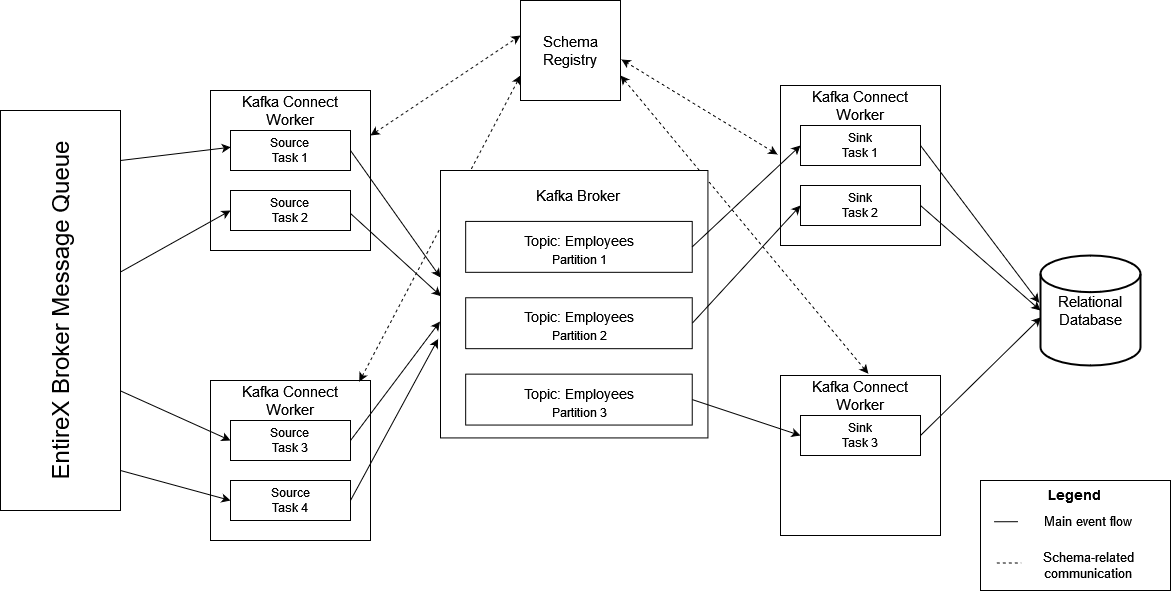
\includegraphics[width=1\textwidth]{chapters/images/kafka pipeline overall architecture enlarged.drawio.png}
 \caption[Overall architecture of Kafka replication pipeline]{Overall architecture of Kafka replication pipeline (see \ref{fig:appendix02:overallarchitecture} for enlarged version)}
 \label{fig:chapter04:overallarchitecture}
\end{figure}

As the solution is intended to be a proof of concept, it is limited in scope. First of all, the solution is currently not intended for full-scale deployment in production. This means that no security measures such as encryption or authorization are supported, and all communication is performed over the \ac{HTTP}. The connectors also lack some functionality due to time constraints, such as no support for replication of coupled files and no support for changes in the \ac{FDT}. Further limitations are discussed in \ref{ch04:pipelinedevelopment:solutionlimitations}.

\section{Implementation Process}
Before the implementation process could properly begin, the design and functionality of Kafka Connect was researched. This involved reading the documentation and looking at available source code of real-life connector implementations. This helped in planning the entire architecture of the solution and the design of the source connector.

\subsection{Implementing the Source Connector}
The main job of the source connector involves consuming any Adabas file change events from the EntireX Broker message queue (see \ref{ch02:fundamentals:adabas:entirex}), transforming the events, and writing them to a specified Kafka topic. There were three main aspects to consider for the connector implementation: how to track changes in the Adabas files, how to divide the work for each task, and how to transform the data to facilitate replication to a relational database further on in the pipeline.
% As explained in \ref{ch02:fundamentals:apachekafkaandkafkaconnect:kafkaconnect}, a connector can run in distributed mode with multiple worker nodes or in standalone mode as a single-process.

\subsubsection{Choosing the Event Replicator as the Source}
There were two strategies being initially considered for tracking Adabas file changes. The first strategy involved adding special \textit{system fields} to the \ac{FDT} that would track the record creation time and the latest change time. The source connector would then be expected to poll the Adabas file at regular intervals and check whether any updates have occurred. This method had major drawbacks, such as the effect that it would have on performance due to regular read commands that would have to be performed. In a production environment where an Adabas file can have over a million records, that can become a major performance bottleneck. This method also fails to identify record deletes. The second strategy, also the one that ended up being implemented, included using the \ac{REPTOR} (see \ref{ch02:fundamentals:adabas:reptor}). Another added advantage of using the \ac{REPTOR} was that the change capture process would be done internally in Adabas, thus minimizing the complexity of the source connector and taking advantage of the mainframe's processing capabilities.

Binary was chosen as the \ac{REPTOR} message format instead of XML due to the performance considerations mentioned in \ref{ch02:fundamentals:adabas:art:limitations}. This required the implementation of a special parser that could interpret the data structures used in the binary format and transform the message into a format that was understood by the connector. The \ac{REPTOR} Parser was implemented to receive an array of bytes representing the message and return the parsed data in the form of a custom DataObject (wrapper class for a HashMap) that contained the message data. The DataObject also contained a custom method for converting the data it contained to a JSON string, adding greater flexibility for further data usage. For a sample binary message and parsed result, see \ref{appendix01:binarymessageexample}.

% \begin{figure}[htbp]
%  \centering
%  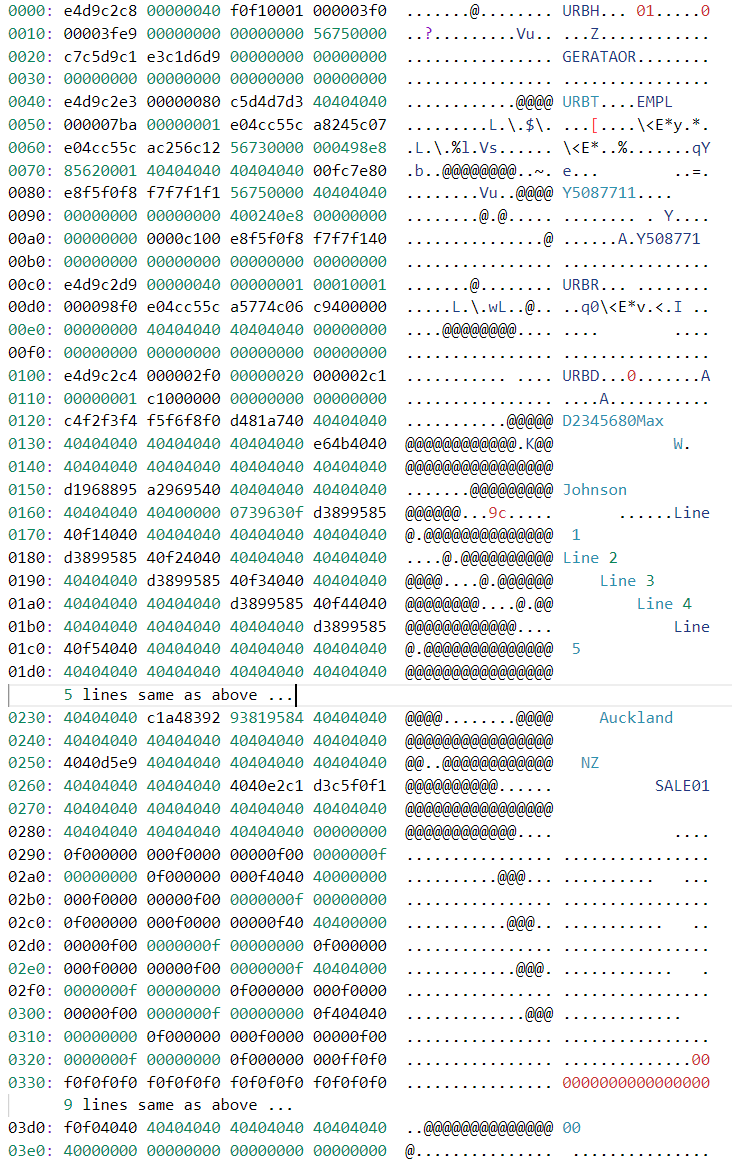
\includegraphics[width=0.49\textwidth]{chapters/images/reptor-parser-binary-light.png}
%  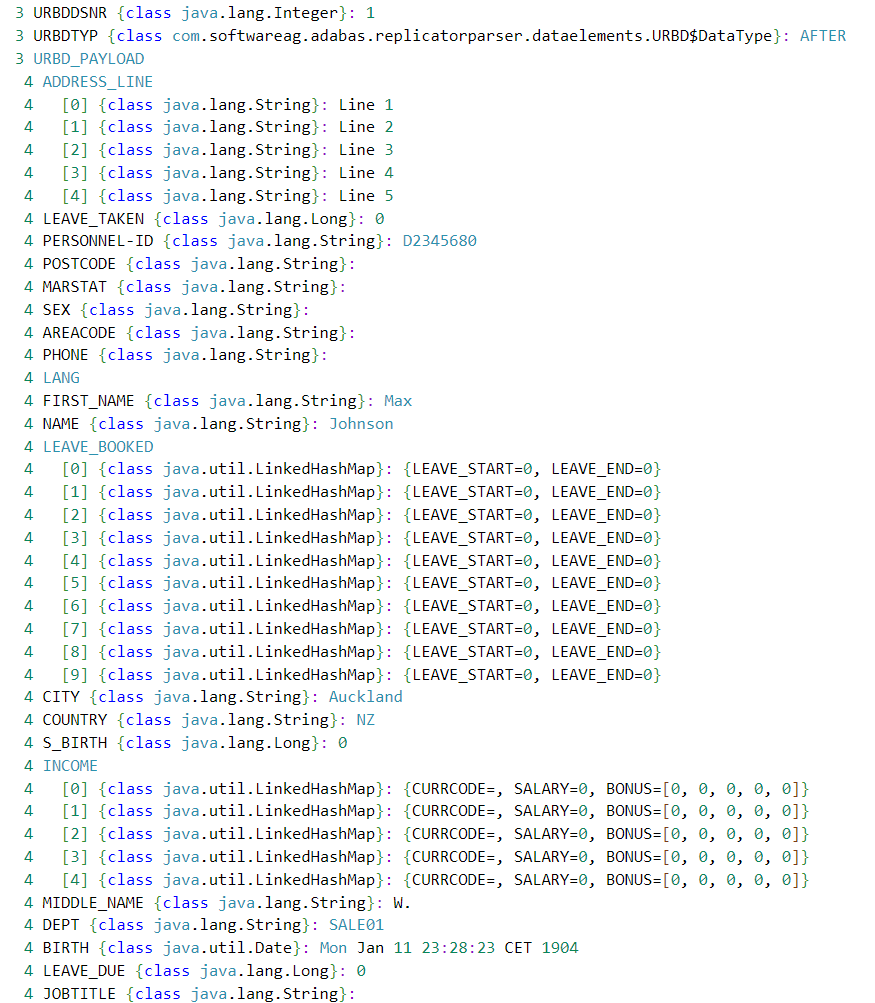
\includegraphics[width=0.49\textwidth]{chapters/images/reptor-parser-parseddataobject-light.png}
%  \caption{Excerpt of a \ac{REPTOR} binary message (left) and the parsed result (right)}
%  \label{fig:chapter04:reptorparserexample}
% \end{figure}
% add to appendix as verbatim

% Figure \ref{fig:chapter04:reptorparserexample} shows the excerpt of a sample binary message and the output of the resulting parsed DataObject. The message in question shows the data image of an Adabas record after an update or insert. Names such as URBDTYP and URBDDSNR represent \ac{REPTOR}-internal data structure fields.

% The second considered strategy included using another Software GmbH product called Adabas Auditing for z/OS. This product also used the EntireX Broker message queue to write auditing events 
% \subsubsection{Writing the Event Replicator Parser} write in upper subsection - to condense

\subsubsection{The Task of Tasks}
To take advantage of Kafka Connect parallelization capabilities, the workload had to be split and distributed to different tasks (the maximum number of tasks is defined in the connector configuration). This is typically done by partitioning the source into different parts and assigning each source partition to one task. However, there was no way to really partition the EntireX Broker message queue. Instead, each task was written to consume from the message queue on a first come first serve basis and process the latest message it received from the queue. Seeing as one \ac{REPTOR} message (or \ac{UOW}) can contain multiple transactions, the task can process multiple events at a time. Each task has an implementation of the \textit{poll} method, which is continuously called and performs the main logic of the task. The polling interval can be specified as a connector configuration.

After the task consumes a \ac{UOW} from the EntireX Broker and parses it with the \ac{REPTOR} Parser, it processes the data and transforms each Adabas record into a number of Kafka records to match the format required for replication to a relational database. The COMMIT message for that specific \ac{UOW} is only sent back to the EntireX Broker after the message has been processed, right before the moment that the Kafka records are returned by the task and written to the Kafka cluster by the connector. Therefore, if the task (or the entire Connect worker) becomes unavailable for any reason while processing a message, the \ac{UOW} will not be marked as processed in the EntireX Broker and can be consumed by another available task in the next poll.
% task processes and only sends commit to broker right before the data is written to kafka 

\subsubsection{Transforming Events to Relational Structure}
\label{ch04:pipelinedevelopment:implementation:transformingtorelational}
To transform an Adabas record to a relational schema, a similar strategy to that of the \ac{ART} default was chosen (see \ref{ch02:fundamentals:adabas:art:schematransformation}). A group field is flattened in the root table, while a new table is generated for each PE group and MU field. However, unlike in the \ac{ART} transformation, no composed index is created of the \ac{ISN} and PE index. Instead, the PE and MU index are set as primary keys additionally to the \ac{ISN} in the respective tables. The root table has the \ac{ISN} as its sole primary key. This was done to enhance table indexing and query performance. Listing \ref{lst:bonusmupequery:connect} shows an example MU field in a PE group generated by the connector, as opposed to the \ac{ART} version shown in Listing \ref{lst:bonusmupequery}. In this case, the primary key fields are the \ac{ISN}, BONUS.IX2, and INCOME.INDEX.

If the schema is auto-generated by the sink connector, no foreign key constraints are created. If foreign key constraints are required, they can either be added manually or the schema can be generated beforehand.
\newpage
\begin{lstlisting}[frame=tb,caption={Query result of the MU field BONUS in the PE field INCOME in the relational table employees\_INCOME\_BONUS (Kafka Connect version)},label=lst:bonusmupequery:connect]
 BONUS | BONUS.IX2 | INCOME.INDEX |  ISN
-------+-----------+--------------+-------
  5000 |         1 |            1 |     1
  2000 |         2 |            1 |     1
  2000 |         3 |            1 |     1
  2500 |         1 |            2 |     1
  2000 |         2 |            2 |     1
\end{lstlisting}
% talk about attempt at using Kafka Streams - leave out for now
% TODO: explain why all messages in one topic

\subsubsection{Writing to Kafka} 
% how were events structured? why all in one topic? how were messages tracked with headers? schema registry?
To write each record to the specified Kafka topic with a message schema, it first has to be constructed as a Kafka Connect-internal "structured record" where the the message structure and content have to be defined, along with a Connect-specific schema definition for that record. The schema is an optional component of Kafka that defines the structure of Kafka messages in a topic. If implemented, the schema can either be sent with every Kafka message, or stored and managed by an additional schema registry. Each schema version has its own ID which also gets stored in each Kafka message, allowing consumers to access the message's specific schema \cite{kafkadatabaseinverted}. This is useful later on for the \ac{JDBC} sink connector, as a way to determine the data types that each field should receive in the target database. The use of schemas is also beneficial in the case that further serialization options, such as Avro, are planned to be added in the future \cite{kreps2011kafka}.

The batch of generated structured records related to the same message are then written to the specified Kafka topic. The message key is set to be the \ac{ISN} of the related Adabas record. Since the default partitioning involves hashing the message key to determine the target partition (see \ref{ch02:fundamentals:apachekafkaandkafkaconnect:apachekafka}), the messages related to the same Adabas record will always end up in the same partition; thus allowing order between the messages for that key to be maintained.
% TODO: add example of message header as verbatim text?

Each Kafka message also contains certain headers which are used to store additional information. One such message header is used for the purpose of determining the table name that each message belongs to\footnote{For instance in the case that the message represents an MU field value.} and the fields that were intended to be primary keys in the target database. Another use for the message header is to track the transaction ID (represented by the transaction commit time), both for tracking the transaction throughput of the sink connector, as well as for identifying which specific transaction the message belongs to. There are other message headers that are generated by the Zipkin service for tracking performance metrics related to each Kafka message (see \ref{ch04:pipelinedevelopment:metrics} for more details). Figure \ref{fig:chapter04:implementation:headerexample} shows a message header containing trace-relevant Zipkin data, as well as the primary key fields and table name. The key can also be seen, showing that this message represents the record with \ac{ISN} 109425.

\begin{figure}[htbp]
 \centering
 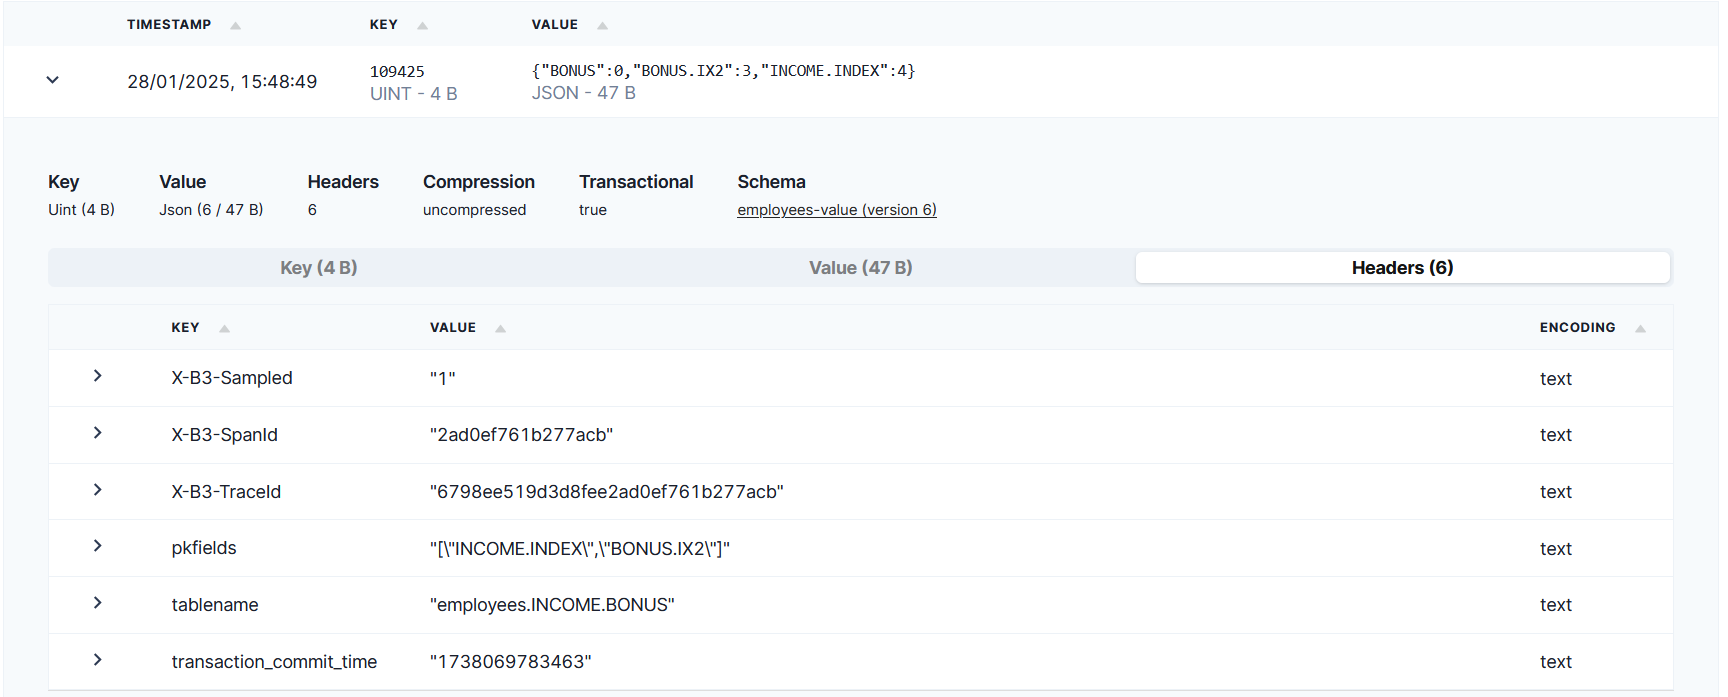
\includegraphics[width=1\textwidth]{chapters/images/header-example.png}
 \caption[Kafka Message with header shown]{Kafka Message with header shown (see \ref{fig:appendix02:implementation:headerexample} for enlarged version)}
 \label{fig:chapter04:implementation:headerexample}
\end{figure}

% TODO: add about transactionality??

\subsection{Implementing the Sink Connector}
Initially, the plan was to implement the \ac{JDBC} sink connector developed by Confluent as it is, without any additional modifications to it. However, some limitations concerning the sink connector cropped up over the course of the implementation, necessitating some modifications to the source code.

\subsubsection{Limitations of Confluent JDBC Sink Connector}
The first limitation encountered by the sink connector was its reliance on topic names to determine the table name in the target database \cite{jdbcsinkdocumentation}. Due to the implementation choice to keep all Kafka records, regardless of the target database table, in the same topic, the sink connector would not have been able to identify the correct target database table name.
% TODO: explain why all messages in one topic further up

Another limitation was the sink connector's inability to set custom primary keys based on the target database table, as is done in \ac{ART}, where MU and PE counters are also treated as primary keys to keep every row identifiable. The available strategies of the sink connector were not meant to handle dynamic primary key definition while allowing the auto-creation of tables and \textit{upserting} of records \cite{jdbcsinkdocumentation}. For more information about the upserting strategy, see \ref{ch04:pipelinedevelopment:parallelizationconsiderations}.

\subsubsection{Modification of Confluent JDBC Sink Connector}
In order to address the sink connector limitations, the source code was pulled and modified. Both the table name and primary key strategy were solved by adding the necessary information to the Kafka message header, providing the sink connector tasks with the necessary information. The source code was then built and Dockerized into a custom image.

\section{Parallelization Considerations}
\label{ch04:pipelinedevelopment:parallelizationconsiderations}
Due to the connectors' distributed nature, aspects such as data consistency and fault tolerance have to be addressed. Due to the source not being partitioned and the tasks in Kafka Connect being designed to run independently of each other, with no way of communicating or synchronizing data, there is guarantee to the order of incoming data and the order that it is written to Kafka by source tasks. For instance, if Task 1 receives a transaction where a record is created, but crashes before processing it, or processes it longer than Task 2 processes a subsequent transaction containing an update on that same record, it is possible that the initial transaction would reach the Kafka broker out of order. This is a challenge generally encountered in distributed systems, where the \ac{CAP} theorem is of great relevance. This theorem states that of the three guarantees listed, only two can be achieved at one time \cite{nookala2022distributedshift}. In the case of our replication solution, an argument can be made that partition tolerance can be theoretically guaranteed between connectors and the Kafka cluster with the configuration of more than one \ac{ISR}. This way, in a scenario where a partition leader node is not reachable, another node can be elected as partition leader \cite{optimizingkafkacap}. Therefore, in line with the theorem, the trade-off can occur either in the availability or the consistency. For this solution, availability was chosen at the cost of strict consistency at the point of the source connector, as afterwards, consistency can be guaranteed by Kafka's offset mechanism. There were two factors that influenced this decision. First of all, if the message order from the source connector proved to be non-negotiable, a further component such as Kafka Streams could be incorporated into the pipeline to handle out-of-order messages before they reach the sink connector \cite{wang2021consistency}. Second of all, in case the order of messages would get mixed up, this wouldn't cause any breaking changes for the sink connector or the target database in the scenario that an update operation of a record would reach the sink connector before the create operation. This is due to the fact that the sink connector has been configured to support \textit{upsert} operations. Thus, if a record is received by the sink connector but does not yet exist in the database, it is inserted instead \cite{jdbcsinkdocumentation}. Furthermore, the \ac{REPTOR} always sends the entire data image of a record, meaning that if a more recent operation reaches the sink connector, the updated state will also contain any changes from previous operations.

% \section{Optimization}
% Some design choices were made in order to optimize the Kafka-based solution.
% not enough for extra section - write about kafka streams in subsection about transforming events to relational structure!

\section{Limitations}
\label{ch04:pipelinedevelopment:solutionlimitations}
% write about transactionality here??
As already demonstrated by the need for custom modifications to the \ac{JDBC} sink connector, there were multiple challenges encountered during the development process. Some of the issues could be resolved with time and effort, while others were too complex to solve in the available time, causing limitations in the scope of this experiment.

The first limitation set is the lack of transactional capabilities of the Kafka solution. While Apache Kafka supports transactionality in the form of "exactly once" delivery guarantees \cite{kafkadocumentation}, not all Kafka Connect components support it. There has been an improvement proposal\footnote{See the Kafka Improvement Proposal 618: \url{https://cwiki.apache.org/confluence/display/KAFKA/KIP-618\%3A+Exactly-Once+Support+for+Source+Connectors}} that adds the "exactly once" delivery guarantee support for source connectors running in distributed mode. However, the \ac{JDBC} sink connector currently only supports the "at least once" delivery guarantee \cite{jdbcsinkdocumentation}. With more time, the \ac{JDBC} sink connector functionality could be extended to provide support for such a delivery guarantee. However, with current available resources, total transaction support had to be left out of the scope. The solution is run with "exactly once" semantics enabled only between the source connector and Kafka brokers.

Another limitation set was the lack of a delete option in the target relational database, as that would have required further development of the custom primary key strategy. The scope was limited only to the create and update operation.

Any changes in the \ac{FDT}, or file schema, were also left out of the scope, as that would require additional tracking and synchronization of any file metadata changes among all the tasks. This can be accomplished in the future with the use of the schema registry service.

Last, but not least, a replication limit of a single Adabas file was set for this scope. While the replication of coupled files could theoretically be accomplished by deploying multiple source connectors (one for each file), this would require further testing.

\section{Metrics}
\label{ch04:pipelinedevelopment:metrics}

\subsection{Monitoring with JMX}
Seeing as Kafka is a Java-based application that runs on the \ac{JVM}, it provides a number of \ac{JMX} metrics with the use of \ac{MBeans}, both for monitoring the system and for basic performance indicators such as broker throughput and latency. Custom metrics can also be added with the \ac{MBeans}, allowing Java applications such as custom connectors to expose metric data relevant to that specific connector. These metrics can then be exposed with the \ac{JMX} exporter agent, allowing them to be collected and evaluated \cite{kafkamonitoringgrafana}. A common stack for monitoring a Kafka-based system involves metric scraping with Prometheus and subsequent visualization (and, if necessary, alerting) with Grafana \cite{applicationmonitoringkafka}.

\begin{figure}[htbp]
 \centering
 \includegraphics[width=1\textwidth]{chapters/images/kafka prometheus monitoring stack enlarged.drawio.png}
 \caption[Monitoring Stack with Prometheus and Grafana]{Monitoring Stack with Prometheus and Grafana (see \ref{fig:appendix02:metrics:prometheusstack} for enlarged version)}
 \label{fig:chapter04:metrics:prometheusstack}
\end{figure}

Figure \ref{fig:chapter04:metrics:prometheusstack} shows an example scenario with two brokers and one Connect worker. Each has a \ac{JMX} exporter running either as part of the application or as a separate Java agent \cite{kafkamonitoringgrafana}. The exporter can be configured to expose certain metrics using a YAML config file, allowing Prometheus to scrape those metrics at regular intervals. Grafana is then used to query the data gathered by Prometheus with the help of \ac{PromQL}, allowing the creation of dashboards for monitoring and data analysis.

% TODO: add screenshot of Grafana dashboard

\subsection{Distributed Tracing}
While \ac{JMX} metrics are useful for monitoring the system as a whole, they typically are not intended for tracing on a per-message basis. Instead, distributed tracing can be implemented with tools such as Zipkin for the tracing of multiple distributed components. In the case of our replication pipeline, a message can be traced with Zipkin from the source connector to the sink connector using the headers in the Kafka message to identify each message. In distributed tracing, a \textit{trace} represents the entire path of the message from the source to the target, while a \textit{span} represents the existence of the message in a specific component of the distributed system \cite{janes2022zipkin}. A trace therefore typically involves multiple spans in a distributed system.

To enable distributed tracing of the Kafka replication solution, an instrumentation library called Brave is used to intercept traces and send them to Zipkin \cite{mallanna2020distributedzipkin}. Such \textit{interceptors} already exist for Kafka Connect in the form of producer and consumer interceptors\footnote{\url{https://github.com/openzipkin-contrib/brave-kafka-interceptor}}. 
Zipkin acts as the collector of the traces and can store them in-memory, or in products with storage and querying capabilities such as Elasticsearch and Cassandra \cite{mallanna2020distributedzipkin}. In this experiment, Elasticsearch was preferred due to existing experience with it. The traces can be indexed and stored in Elasticsearch, then queried and visualized with Kibana. % TODO: add diagram of zipkin

The available interceptors for Kafka Connect allow for the tracing of each produced and consumed Kafka message. To also enable tracing of the entire transaction (which consists of multiple Kafka messages), a custom Zipkin trace was implemented in the source and sink connectors using the Brave library. This allows for the custom metric to measure the throughput transaction of both connectors.


% - JMX good for single components

% - tracing every separate message from start to end, use zipkin

% - measure throughput based on separate records or based on transactions

% Custom JMX metrics in source connector, using existing JMX metrics of all components - some comparable to ART. Using Zipkin for distributed tracing.
\chapter{Experiment Methodology}
\label{ch05:methodology}
To address the research question \textbf{"How does the performance of a Kafka Connect-based replication pipeline for Adabas on mainframe compare to the Adabas Event Replicator Target Adapter?"}, an experiment was conducted to test the performance of both systems. As the hypothesis states that the Kafka-based solution will outperform \ac{ART} only when its performance capabilities are leveraged, the experiment was designed in a way to take into account different parallelization configurations of the Kafka replication pipeline.

\section{Experiment Design}
\label{ch05:methodology:design}
The experiment involved generating a large volume of create or update changes in Adabas to test the throughput of both systems over a period of time. Due to \ac{ART} being run on one machine, while the replication pipeline is distributed, two throughput metrics were chosen that provide comparable results. These are the number of \textbf{transactions per second}, as well as \textbf{messages per second}. For the scope of this experiment, only the performance of Kafka-related components that processed the replication data was measured. This included the source and sink connector workers, as well as the Kafka brokers. The schema registry's performance was not measured, as it was used as an additional service and did not affect the replication data's throughput.

\subsection{Defining the Metrics}
In the case of Kafka replication, \textit{messages} refer to the number of total Kafka events transferred in the pipeline. As explained in \ref{ch04:pipelinedevelopment:implementation:transformingtorelational}, due to each Adabas record being normalized and split into smaller records in the source connector, there is more message traffic in the replication pipeline than just the single Adabas record. This made it difficult to compare it to the way that \ac{ART} works, as \ac{ART} processes the entire \ac{REPTOR}'s XML message that it receives and transforms the records internally before writing them to the target database. To have a comparable metric of messages per second, it was instead tracked by how many \textit{table rows}, which are identical to the split records in Kafka, were created by \ac{ART} and written to the target database.

The transaction throughput metric was more straightforward, as both solutions process the same total number of transactions. However, as mentioned in \ref{ch04:pipelinedevelopment:solutionlimitations}, transactionality is only supported by the source connector. Therefore, the transaction throughput was only measured for the source connector and compared with the \ac{ART} throughput for an approximate comparison.

\subsection{Measuring the Metrics}
The message and transaction throughput of the Kafka source connector and \ac{ART}, as well as the message throughput of the sink connector, were measured with Zipkin. In the case of the Kafka connectors, there is already built-in Zipkin support using so-called Kafka interceptors\footnote{\url{https://github.com/openzipkin-contrib/brave-kafka-interceptor}} to capture the Zipkin traces. For \ac{ART} and for transaction tracing, custom Zipkin traces were implemented using the Brave\footnote{\url{https://github.com/openzipkin/brave}} library. To measure the message throughput of the Kafka brokers, \ac{JMX} metrics were used. Unfortunately, the existing \ac{JMX} metrics did not support measuring the transaction throughput of the brokers. Therefore, the performance metrics were evaluated without taking into account the broker transaction throughput. If the broker(s) become the bottleneck, this can still be identified by monitoring the message throughput.

% The experiment is operating under the assumption that the Kafka brokers will not be the performance bottleneck in the replication pipeline if the brokers are configured in a way to optimize parallelization. This can be done by increasing the number of partitions in the Kafka topic, allowing throughput to be increased through a higher degree of parallelization \cite{cerezo2021analysisparallelism}. Therefore, the performance metrics will be evaluated without taking into account the broker transaction throughput.
% can look at byte throughput of entire kafka system (not comparable to art though) to see which system is the bottleneck?

The experiment was also intentionally designed to measure the throughput of components up until the data reached the \ac{JDBC} driver. This allows for the disregard for any latencies that result from the upsert operations to the target database. The target relational database used for the experiment was Postgres as a result of existing familiarity with it.
% maybe include that want to isolate performance and not include database variability - however, database can still be a bottleneck

\subsection{Initial State Data}
Due to the upsert nature of the \ac{JDBC} sink connector (see \ref{ch04:pipelinedevelopment:parallelizationconsiderations}), there is no real difference between the insert and update operations for the replication pipeline, therefore their performance does not need to be tested separately. Since the latencies with respect to the target database operations and any delete operations are outside of the scope, the \ac{IS} operations were used to simulate a high-throughput situation. This made it easier to prepare the Adabas file beforehand, as the data had to be inserted only once, and there was no need to delete or re-insert records in Adabas for every experiment run. This helped not only with saving time between each run, but also with reproducibility, as the number of records, record content, and generated \ac{REPTOR} message structures remained the same for every test run. The only difference in the messages resulted from \ac{ART} requiring the XML format, while the source connector required the binary format.

\subsection{Kafka Replication Scenarios}
\label{ch05:methodology:design:scenarios}
There were different Kafka pipeline setups tested against the \ac{ART} solution, to see whether or not parallelization would play a decisive factor in outperforming \ac{ART}, and to see which pipeline setup will ensure maximum performance. Each scenario was run and measured five times to minimize possible variability. The same was done for measuring the performance of \ac{ART}. The scenarios were as follows:
\begin{description}
    \item [One Task, One Partition]
    First, the performance of the replication pipeline was tested without any parallelism involved: the source and sink connectors were run on one Connect worker each, with only one task each. There was a single Kafka broker with only one partition.

    \item[Three Tasks on One Worker, Three Partitions]
    This scenario tested the parallelization capabilities of Kafka. There were three source tasks and three sink tasks. Two workers were used in total, one for the sink connector and one for the source connector. There were also three brokers, each broker being assigned partition leader for a single partition.

    \item[Seven Tasks on One Worker, Seven Partitions]
    This scenario tested the parallelization capabilities of Kafka to a higher degree than in the previous scenario. There were seven source tasks and seven sink tasks, run on one worker each. Seven partitions were configured, balanced among three brokers. The broker number was kept at three to test whether the brokers could handle a higher partition number\footnote{According to a Confluent blog post, a single Kafka broker can handle multiple thousand partitions and still maintain high availability (\url{https://www.confluent.io/blog/how-choose-number-topics-partitions-kafka-cluster/}).}.

    \item[Seven Tasks on Two Workers, Seven Partitions]
    This scenario was similar to the previous one. In this case, however, the seven source tasks and seven sink tasks were balanced on two Connect workers for the source and sink connector each (with four workers in total). The aim was to provide an insight into whether the distribution of tasks would provide additional throughput improvements.
    
    \item[20 Tasks on Five Workers, 20 Partitions] The last scenario used a significant increase in parallelization. It was selected to see whether the performance would scale effectively. The source and sink connectors were run on 5 workers each, with 20 tasks assigned per connector. The 20 partitions were hosted on three brokers.
    
\end{description}

The different scenarios can be compared to various Kafka Connect set-up types. The first scenario is often used for initial development without parallelization, while the second scenario represents a typical non-production test environment. The last three scenarios can be considered as variations of production environments, depending on workload and performance requirements. % Typically, configuration based on performance necessities and data volume - here that is not the case, as want to portray different scenarios -> CITE!!

In production environments, it is always recommended to enable partition replication on multiple brokers for additional fault tolerance. In the case of this experiment, no replication was enabled, to minimize its effect on Kafka's performance \cite{dobbelaerekafkavsrabbitmq}.

The number of tasks per connector and topic partitions was kept the same in order to take full advantage of the parallelization that partitions offer. An odd number of brokers were used for the KRaft leadership elections to work properly \cite{kraftconfluentdocumentation}.

% talk about # of tasks per partition (or vice versa) - tasks partition wise for jdbc connector?

% what configurations of kafka will be tested?

% \section{Pipeline Configuration}
% \label{ch05:methodology:pipelineconfiguration}
% \newpage
\section{Adabas File}
\label{ch05:methodology:adabasfile}
One Adabas file was used for testing the replication performance. It is called \textit{EMPLOYEES}, and contains sample employee data. This file was chosen because it has all of the existing field types described in \ref{ch02:fundamentals:adabas:forzos:datastructures}. It contained 171405 total records. Below is the \ac{FDT} showing all of the fields that will be replicated to the target database:
\begin{verbatim}
Field Description Table: File 1     (EMPLOYEES)                              
========================                Total Fields without SDT ... 31      
*************** T o p  of  F D T ***************                             
Lev  I Name I Leng  I Form  I    Options       I Predict Fld Name or DT / SY 
-----I------I-------I-------I----------------- I-----------------------------
  1  I  AA  I  008  I    A  I  DE UQ           I   PERSONNEL_ID              
  1  I  AB  I       I       I                  I   FULLNAME                  
  2  I  AC  I  020  I    A  I  NU              I   FIRST_NAME                
  2  I  AE  I  020  I    A  I  DE              I   NAME                      
  2  I  AD  I  020  I    A  I  NU              I   MIDDLE_NAME               
  1  I  AF  I  001  I    A  I  FI              I   MARSTAT                   
  1  I  AG  I  001  I    A  I  FI              I   SEX                       
  1  I  AH  I  004  I    P  I  DE NC           I   BIRTH                     
  1  I  A1  I       I       I                  I   FULL_ADDRESS              
  2  I  AI  I  020  I    A  I  MU NU           I   ADDRESS_LINE              
  2  I  AJ  I  020  I    A  I  DE NU           I   CITY                      
  2  I  AK  I  010  I    A  I  NU              I   POSTCODE                  
  2  I  AL  I  003  I    A  I  NU              I   COUNTRY                   
  1  I  A2  I       I       I                  I   TELEPHONE                 
  2  I  AN  I  006  I    A  I  NU              I   AREACODE                  
  2  I  AM  I  015  I    A  I  NU              I   PHONE                     
  1  I  AO  I  006  I    A  I  DE              I   DEPT                      
  1  I  AP  I  025  I    A  I  DE NU           I   JOBTITLE                  
  1  I  AQ  I       I       I  PE              I   INCOME                    
  2  I  AR  I  003  I    A  I  NU              I   CURRCODE                  
  2  I  AS  I  005  I    P  I  NU              I   SALARY                    
  2  I  AT  I  005  I    P  I  MU NU           I   BONUS                     
  1  I  A3  I       I       I                  I   LEAVE_DATA                
  2  I  AU  I  002  I    U  I                  I   LEAVE_DUE
  2  I  AV  I  002  I    U  I  NU              I   LEAVE_TAKEN               
  1  I  AW  I       I       I  PE              I   LEAVE_BOOKED              
  2  I  AX  I  008  I    U  I  NU              I   LEAVE_START               
  2  I  AY  I  008  I    U  I  NU              I   LEAVE_END                 
  1  I  AZ  I  003  I    A  I  DE MU NU        I   LANG                      
  1  I  BA  I  014  I    U  I  NU CR           I   INSERT                    
  1  I  BB  I  014  I    U  I  MU NU           I   UPDATE                    
\end{verbatim}

The \textit{Name} field refers to the Adabas file shortnames, which are used internally to identify the fields. Each shortname can have a longname mapped to it (shown in the \ac{FDT} as \textit{Predict Fld Name}). \textit{Form} shows the format of the fields: \textbf{A}lphanumeric, \textbf{P}acked decimals, and \textbf{U}npacked decimals. \textit{Lev} indicates the nested level of a field: for instance, ADDRESS\_LINE is a multiple field that is nested in the FULL\_ADDRESS group. Meanwhile, the \textit{Options} field describes field attributes. The relevant options include MU and PE, which indicate whether the field is a multiple field or a periodic group.

\section{Environment Setup with Azure}
\label{ch05:methodology:environmentsetup}
The experiment was chosen to run on the Azure Cloud platform to simulate a production environment. Each Kafka broker, Connect worker and \ac{ART} instance was run on a separate \ac{VM} provisioned in Azure, while Adabas and \ac{REPTOR} were run on a Software GmbH mainframe. Azure was chosen because of an existing corporate subscription and existing infrastructure. This included an existing connection to the Software GmbH intranet for access to Adabas, as well as an existing subnet and virtual network.

\subsection{Ensuring Reproducibility}
Multiple measures were taken to ensure the reproducibility of the results and to control as many variables as possible to minimize variability. Terraform was chosen as an \ac{IaC} tool to allow the provisioning of a testing infrastructure, allowing it to be reproduced at will. This allowed more control over the provisioning of \ac{VM}s, as well as the management of the testing environment.

The Ubuntu Server distribution was chosen as the \ac{OS} for all \ac{VM}s due to its open source nature. All applications were containerized using Docker, allowing ease of setup and ensuring consistent and isolated environments for each experiment run. Using Docker simplified the task of stopping and starting new instances of all applications between experiment repetitions, ensuring that previous measurements and actions did not affect the performance of subsequent runs.

To control for the effect of hardware on performance, the \ac{VM}s used for hosting \ac{ART} and the Kafka pipeline components were all provisioned with the same specifications. The Azure D-series \ac{VM} was used, as it is optimized for general-purpose production workloads\footnote{\url{https://azure.microsoft.com/en-us/pricing/details/virtual-machines/series/}}. Table \ref{tab:hardwarespecs} lists the important hardware specifications. The Postgres database was run on a machine with identical hardware.


\begin{table}
    \centering
    \begin{tabular}{|cc|}
        \hline
         \textbf{Operating System} & Ubuntu Server 22.04 LTS \\
         \textbf{Processor} & AMD EPYC 7763 64-Core \\
         \textbf{Memory} & 16 GiB \\
         \textbf{vCPUs} & 4 \\
        \hline
    \end{tabular}
    \caption{Hardware Specifications for Performance Tests}
    \label{tab:hardwarespecs}
\end{table}

% - using terraform

% - multiple experiment runs for each scenario (take average?)

% - restarting VMs for every experiment run
% use of terraform, restarting every time with fresh kafka brokers and connectors - only metrics collection is kept running?


\subsection{Kafka-based Solution}
For the Kafka Connect pipeline, each Connect worker and Kafka broker were run on a separate \ac{VM} to simulate nodes in an actual cluster. An additional \ac{VM} with the same specifications was provisioned as the "control \ac{VM}" to host the schema registry and a web UI of the Kafka cluster. Even when running a single worker for the first experiment scenario, the worker was still run in distributed mode\footnote{The "Exactly Once" semantic in the source connector is only available when running in distributed mode (see \ref{ch04:pipelinedevelopment:solutionlimitations}).}. Listing \ref{lst:terraform} shows an example Terraform script used to provision a source connect worker.

\subsection{Target Adapter}
As \ac{ART} does not support parallelization, it was run as a single \ac{VM} instance with the same specifications shown in Table \ref{tab:hardwarespecs}. The message and transaction throughput was tracked using Zipkin and Elasticsearch.

\subsection{Metrics Collection}
The metrics collection was performed using Grafana and Prometheus for the \ac{JMX} metrics, and Zipkin, Elasticsearch, and Kibana for the message and transaction tracing. Due to the high \ac{CPU} and memory requirements for Zipkin and Elasticsearch, all metrics collection was hosted on an on-premise machine with a high amount of available memory. All components were also started as Docker containers. The Elasticsearch cluster was configured with three nodes to handle the high volume in message traces that had to be collected.
\chapter{Results and Analysis}
\label{ch06:resultsandanalysis}

\section{Quantitative Results}
\label{ch06:resultsandanalysis:quantitativeresults}

\section{Qualitative Observations}
\label{ch06:resultsandanalysis:qualitativeobservations}

\section{Scalability and Architectural Considerations}
\label{ch06:resultsandanalysis:scalabilityconsiderations}
\chapter{Analysis and Discussion}
\label{ch07:discussion}
% Introduction to results - what were the experiment findings?
As demonstrated in Chapter \ref{ch06:results}, the Kafka Connect replication pipeline outperformed the Target Adapter even when no parallelization was implemented. The findings support the hypothesis outlined in Chapter \ref{ch05:methodology}, to the extent that leveraging parallelization had a positive impact on performance when compared to \ac{ART}. However, the additional predication that \ac{ART} would surpass Kafka Connect replication in single-threaded mode proved to be false. This chapter discusses the results and their implications in depth, and analyzes the effect of different factors on performance.

\section{Statistical Significance}
\label{ch07:discussion:statsig}
The confidence interval is used for determining the statistical significance of all average throughput measurements. It is also used to determine whether scenarios statistically differ from each other. The confidence level was set to 90\%, in accordance with the strategy outlined by \citeauthor{jain1991computer} \cite{jain1991computer}. The interval is typically inversely affected by the sample size and directly affected by variability and confidence level \cite{hazrausingci}. Since the sample size of five and confidence level are relatively low in the case of this experiment, any narrow intervals can most likely be attributed to low data variability. This will be regarded as true for all subsequent discussion. In the case of wide intervals, the same logic cannot be applied.

\subsection{Target Adapter}
The confidence interval for \ac{ART} is visualized in Figure \ref{fig:chapter07:discussion:artci}. The message throughput in Figure \ref{fig:chapter07:discussion:artavgmessageci} has error bars approximately between 1.91K and 1.96K, showing a relatively narrow interval. The narrow interval could be due to low variability in the measured data. The low variability is also supported by the small difference between the mean and median in Table \ref{tab:art:messagethroughput}.

Figure \ref{fig:chapter07:discussion:artavgtransci} shows the confidence interval for \ac{ART}'s total transaction throughput. It contains no visible bars, indicating that the interval is extremely narrow with only a 0.002 difference. This is supported by a very low standard error of 0.076 and no difference between the mean and median in Table \ref{tab:art:transactionthroughput}. A possible effect could be low data variability due to the throughput occurring in bursts instead of continually. Possible reasons for this behavior will be elaborated upon in \ref{ch07:discussion:performancevariability}.

\begin{figure}[htbp]
    \centering
    \subfloat[Message throughput confidence interval]{\label{fig:chapter07:discussion:artavgmessageci}
        \centering
        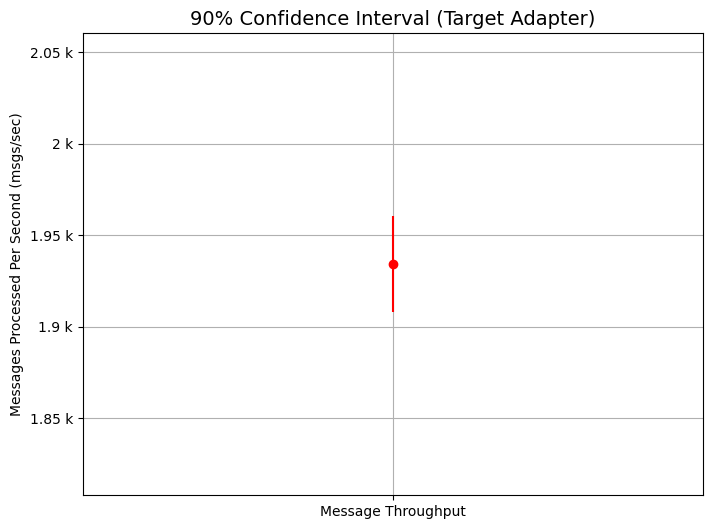
\includegraphics[width=0.75\textwidth]{chapters/images/confidence-intervals/art-message-ci.png}
    }
    \hfill
    \subfloat[Transaction throughput confidence interval]{\label{fig:chapter07:discussion:artavgtransci}
        \centering
        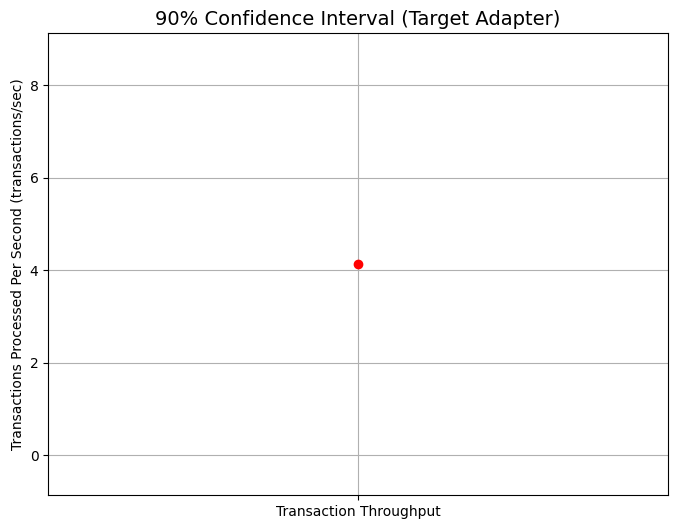
\includegraphics[width=0.75\textwidth]{chapters/images/confidence-intervals/art-transaction-ci.png}
    }
    \hfill
    \caption{Target Adapter throughput confidence interval}
    \label{fig:chapter07:discussion:artci}
\end{figure}

\subsection{Source Connector}
The source connector's confidence interval for both the message and transaction throughput is visualized in Figure \ref{fig:chapter07:discussion:sourceci}. The interval for Scenario 1 in Figure \ref{fig:chapter07:discussion:sourcemessageci} is also too narrow to be seen, with bounds between approximately 26.3K and 27.8K. This could also be the result of low data variability. The rest of the scenarios also have relatively narrow intervals, with the widest interval being between 124K and 133K for Scenario 5. All scenarios are significantly different from each other based on a visual test of the confidence intervals \cite{jain1991computer}, with Scenario 2 and Scenario 3 only marginally passing that test.

\begin{figure}[htbp]
    \centering
    \subfloat[Message throughput confidence interval]{\label{fig:chapter07:discussion:sourcemessageci}
        \centering
        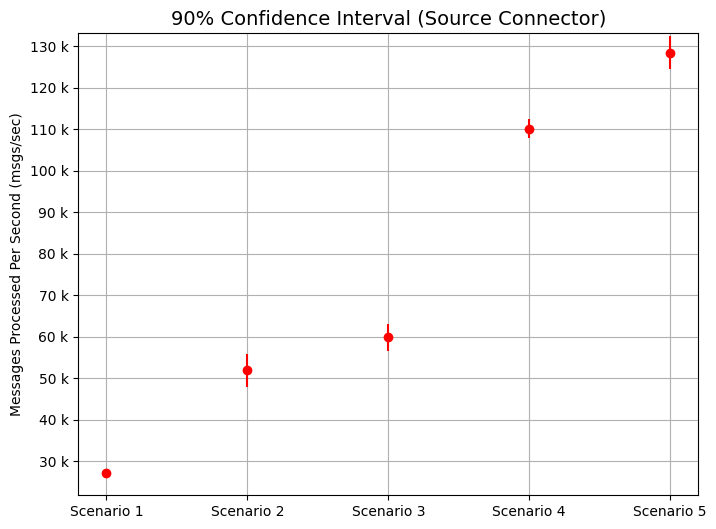
\includegraphics[width=0.75\textwidth]{chapters/images/confidence-intervals/source-message-ci.png}
    }
    \hfill
    \subfloat[Transaction throughput confidence interval]{\label{fig:chapter07:discussion:sourcetransci}
        \centering
        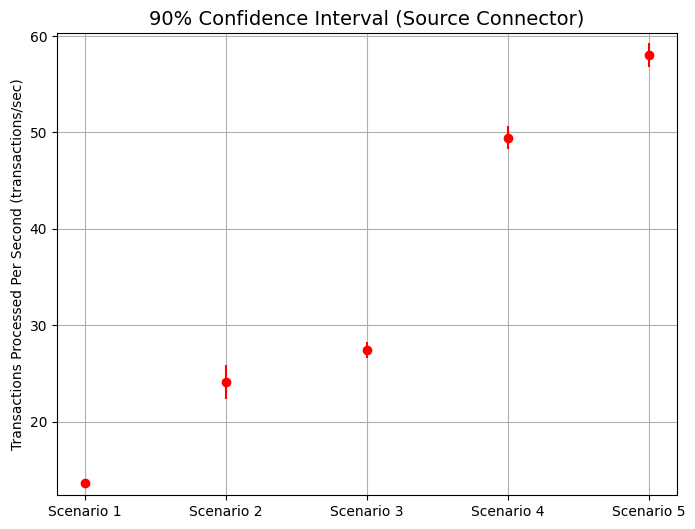
\includegraphics[width=0.75\textwidth]{chapters/images/confidence-intervals/source-transaction-ci.png}
    }
    \hfill
    \caption{Source connector throughput confidence interval}
    \label{fig:chapter07:discussion:sourceci}
\end{figure}

The confidence interval for the transaction throughput can be seen in Figure \ref{fig:chapter07:discussion:sourcetransci}. Just as in Figure \ref{fig:chapter07:discussion:sourcemessageci}, Scenario 1 has a small enough interval to not be visible on the visualization. The rest of the intervals have intervals of approximately 2-3 transactions in size. The largest interval was recorded in Scenario 2, with a bound between 22.4 and 25.8 transactions. The measurements in all scenarios are statistically different from each other, indicating a statistically significant increase in transaction throughput with each scenario.

\subsection{Broker}
The confidence interval for the broker's average message throughput can be found in Figure \ref{fig:chapter07:discussion:brokermessageci}. Scenarios 1 and 4 have no visible intervals, indicating a possibly low variation in the measured throughput. Scenario 5 has an uncommonly large interval between approximately 105K and 131K. It is unlikely for data variability to have played a role in this case, as the difference between the mean and median for Scenario 5 is not much different than for Scenario 4 in Table \ref{tab:kafka:messagethroughputbroker}, while the boundary size differs significantly. It is possible that the sample size of all runs to calculate the average of Scenarios 4 and 5 are too small, as the broker's activity duration was less than 1.5 minutes (see Figure \ref{fig:chapter06:results:brokerallscenarios}). This could have led to discrepancies in the estimation and standard error.

\begin{figure}[htbp]
    \centering
    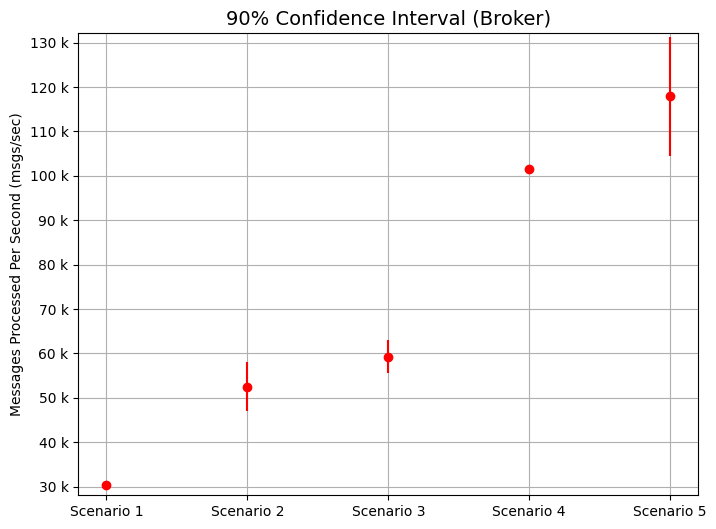
\includegraphics[width=0.75\textwidth]{chapters/images/confidence-intervals/broker-message-ci.png}
    \caption{Broker message throughput confidence interval}
    \label{fig:chapter07:discussion:brokermessageci}
\end{figure}

The boundaries of Scenario 2 and Scenario 3 overlap. A t-test was performed with the resulting p = 0.0673, indicating that the difference between them is not statistically significant. The other scenarios differ from each other significantly, proving that in most cases the performance improved significantly with higher parallelization.

\subsection{Sink Connector}
Figure \ref{fig:chapter07:discussion:sinkmessageci} shows the confidence interval results for the sink connector's message throughput. The boundaries are too narrow to be visible for Scenarios 1-3, possibly due to low throughput variability. This is also supported visually by Figure \ref{fig:chapter06:results:sinkallscenarios} and by comparing the mean and median in Table \ref{tab:kafka:messagethroughputsink}. The boundaries for Scenario 4 and Scenario 5 are higher. However, they are still relatively narrow. This is unexpected for Scenario 5 especially, as it contains very high variability in Figure \ref{fig:chapter06:results:sinkallscenarios} and a very high difference between the mean and median in Table \ref{tab:kafka:messagethroughputsink}. A possible explanation could be similar to that of the broker, as the sink's activity in Scenario 5 was also less than 1.5 minutes, leading to a very small window of measurements.

\begin{figure}[htbp]
    \centering
    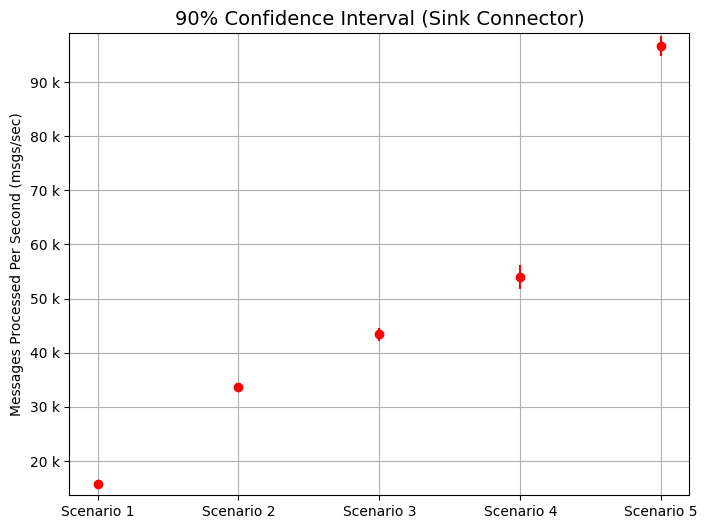
\includegraphics[width=0.75\textwidth]{chapters/images/confidence-intervals/sink-message-ci.png}
    \caption{Sink connector message throughput confidence interval}
    \label{fig:chapter07:discussion:sinkmessageci}
\end{figure}

All of the scenarios are significantly different from each other based on visual evaluation, indicating that parallelization had a statistically significant impact on the performance in all measured scenarios.

\section{Effects of Parallelization}
Overall, the confidence intervals discussed in \ref{ch07:discussion:statsig} showed that the increase in parallelization had a statistically significant impact on the performance of all components in the Kafka replication pipeline. The source connector and the broker experienced the most significant improvement in throughput in Scenario 4, when the same number of tasks that were run in Scenario 3 were distributed on two workers in the source connector. This speaks not only to the positive impact of parallelization, but also to that of distributed processing. The increase in the broker's performance, despite no changes to its configuration, shows that the broker's performance scaled with the source connector. % add screenshots of cpu usage?

The same effect of distribution was not observed for the sink connector. As seen in Figure \ref{fig:chapter07:discussion:sinkmessageci}, the distribution of tasks to an additional worker improved the performance slightly. Nevertheless, the most significant performance increase occurred in Scenario 5, when additional workers and more than double the number of tasks were added to the sink connector. This shows that the sink connector could require a higher degree of parallel processing to achieve similar results to the source connector. However, at approximately 97K messages per second, the sink connector is still below the source connector's performance in Scenario 4 and Scenario 5. This leads to the possibility that the Postgres database is the actual bottleneck, and that latencies related to the upsert operations influence the performance of individual tasks. This would explain why increasing the number of tasks increases the performance more drastically than increasing the number of workers: the more tasks, the more operations can be performed despite connector or database latencies. It would be interesting for further research to investigate whether different database configurations or even different relational databases would affect the sink connector's performance. More testing would also be required to determine the optimal degree of parallelization for the source connector.

Scenario 5 proved to have an unexpected result for the source connector (and, by extension, the broker). It was expected that such a significant increase in tasks and workers would result in a more significant improvement in performance. A possible reason for that could be that the EntireX Broker queue becomes the bottleneck and cannot handle the high number of parallel tasks. A possible solution for that could be to configure multiple queues, each of which is responsible for a certain range of \ac{ISN}s. This would allow for the performance of the EntireX Broker to scale together with the performance of the source connector. It would be interesting to run more tests in the future to determine the load limit of a single EntireX Broker queue and the effect of multiple queues on overall performance.

\section{Scalability and Architectural Considerations}
% very scalable, however increased complexity, need to manage cluster and its health
% mention in prev section that performance bottleneck may exist - then clarify here that scalable up to a certain extend, what else can be done to improve that scalability (multiple queues, more jdbc tasks, etc.)
As the various scenarios have shown, the Kafka replication pipeline is extremely scalable, allowing the degree of parallelization to be increased with ease. However, as discussed in the previous section, there is the possibility of other bottlenecks in the system, such as the EntireX Broker queue and the Postgres database. The EntireX Broker can be scaled, as discussed, by adding additional queues for processing specific \ac{ISN} ranges. With regards to Postgres, the results of Scenario 5 showed that a large number of tasks had a more positive impact on the sink connector's performance. Database query and insertion latency could be the culprit, in which case scaling the sink connector to a greater degree than the source connector could be of benefit. If, however, further scaling of the sink connector does not improve performance, it might be helpful to consider running Postgres as a distributed database. This would allow for Postgres to be scaled along with the Kafka replication and with the EntireX Broker, improving not only scalability but also availability of the database. A possible strategy for scaling Postgres is with Citus, a database engine that allows for Postgres to be run and scaled as a distributed database \cite{cubukcu2021citus}.

Overall the scalability of the Kafka replication solution is a major advantage compared to \ac{ART}, as it can improve overall performance and guarantee availability. However, as with any distributed system, there is also its complexity to consider. While the performance increase might be beneficial, there is also the maintenance of the Kafka cluster to consider in a production environment. This requires constant monitoring of the cluster's health, especially in case nodes become unavailable or any unknown errors cause tasks to fail and crash. This requires additional resources, not to mention the cost for hosting such a cluster around the clock. It is therefore important to consider whether the additional cost and maintenance effort are worth the required increase in performance and scalability. The Kafka-based solution might be especially attractive for companies with an existing Kafka cluster, since they already have an existing infrastructure and trained specialists to monitor and maintain the entire replication pipeline.

\subsection{The Consistency vs. Performance Trade-off}

\section{Performance Variability}
\label{ch07:discussion:performancevariability}
% variability - different number of transactions/Adabas records per EntireX broker message - partial cause?
% dockerization, garbage collection - drops in performance
% entirex broker and postgres bottleneck?

\section{Experiment Limitations}
% only initial state tested for "consistent" results and similarity - interesting how updates would affect, as art doesn't receive full data image
% interesting in future to test flat fields only or more periodic fields

\chapter{Conclusion}
\label{ch08:conclusion}

\section{Further Considerations}
%*************************************************************************
% Recommendations
%*************************************************************************
%\part{Empfehlungen zur Erstellung wissenschaftlicher Abschlussarbeiten}
%\label{pt:recommendations}
%*************************************************************************
% Backmatter
%*************************************************************************
\appendix
%\renewcommand{\thechapter}{\alph{chapter}}
\cleardoublepage
\part{Appendix}
\chapter{Additional Samples}

\section{Binary Message Example}
\label{appendix01:binarymessageexample}
\ref{appendix01:binarymessageexample:binarymessage} shows the hexdump of a sample binary message, with a readable preview on the right. The message in question shows the "after image" of the Adabas record after an insert operation. It is then parsed into a custom DataObject type. The console dump of this object can be seen in \ref{appendix01:binarymessageexample:parsedmessage}. Names such as URBDTYP and URBRISN represent \ac{REPTOR}-internal data structure fields. For instance, URBRISN indicates the \ac{ISN} of the record being displayed, while URBTTTIM indicates the exact time of the transaction commit for this record. Fields that are in groups, such as LEAVE\_DUE and LEAVE\_TAKEN (in group LEAVE\_DATA), are flattened and treated as level-1 fields. Meanwhile, MUs such as ADDRESS\_LINE are represented by an array, while the PE field LEAVE\_BOOKED is represented as an array of objects (LinkedHashMaps to retain the order of occurrences). For the \ac{FDT} that defines all of the field names, see \ref{ch05:methodology:adabasfile}.

\subsection{Event Replicator Binary Message}
\label{appendix01:binarymessageexample:binarymessage}
\begin{verbatim}
0000: e4d9c2c8 00000040 f0f10001 000003f0  .......@........ URBH... 01.....0
0010: 00003fe9 00000000 00000000 56750000  ..?.........Vu.. ...Z............
0020: c7c5d9c1 e3c1d6d9 00000000 00000000  ................ GERATAOR........
0030: 00000000 00000000 00000000 00000000  ................ ................
0040: e4d9c2e3 00000080 c5d4d7d3 40404040  ............@@@@ URBT....EMPL    
0050: 000007ba 00000001 e04cc55c a8245c07  .........L.\.$\. ...[....\<E*y.*.
0060: e04cc55c ac256c12 56730000 000498e8  .L.\.%l.Vs...... \<E*..%.......qY
0070: 85620001 40404040 40404040 00fc7e80  .b..@@@@@@@@..~. e...        ..=.
0080: e8f5f0f8 f7f7f1f1 56750000 40404040  ........Vu..@@@@ Y5087711....    
0090: 00000000 00000000 400240e8 00000000  ........@.@..... ........ . Y....
00a0: 00000000 0000c100 e8f5f0f8 f7f7f140  ...............@ ......A.Y508771 
00b0: 00000000 00000000 00000000 00000000  ................ ................
00c0: e4d9c2d9 00000040 00000001 00010001  .......@........ URBR... ........
00d0: 000098f0 e04cc55c a5774c06 c9400000  .....L.\.wL..@.. ..q0\<E*v.<.I ..
00e0: 00000000 40404040 40404040 00000000  ....@@@@@@@@.... ....        ....
00f0: 00000000 00000000 00000000 00000000  ................ ................
0100: e4d9c2c4 000002f0 00000020 000002c1  ........... .... URBD...0.......A
0110: 00000001 c1000000 00000000 00000000  ................ ....A...........
0120: c4f2f3f4 f5f6f8f0 d481a740 40404040  ...........@@@@@ D2345680Max     
0130: 40404040 40404040 40404040 e64b4040  @@@@@@@@@@@@.K@@             W.  
0140: 40404040 40404040 40404040 40404040  @@@@@@@@@@@@@@@@                 
0150: d1968895 a2969540 40404040 40404040  .......@@@@@@@@@ Johnson         
0160: 40404040 40400000 0739630f d3899585  @@@@@@...9c.....       ......Line
0170: 40f14040 40404040 40404040 40404040  @.@@@@@@@@@@@@@@  1              
0180: d3899585 40f24040 40404040 40404040  ....@.@@@@@@@@@@ Line 2          
0190: 40404040 d3899585 40f34040 40404040  @@@@....@.@@@@@@     Line 3      
01a0: 40404040 40404040 d3899585 40f44040  @@@@@@@@....@.@@         Line 4  
01b0: 40404040 40404040 40404040 d3899585  @@@@@@@@@@@@....             Line
01c0: 40f54040 40404040 40404040 40404040  @.@@@@@@@@@@@@@@  5              
01d0: 40404040 40404040 40404040 40404040  @@@@@@@@@@@@@@@@                 
      5 lines same as above ...
0230: 40404040 c1a48392 93819584 40404040  @@@@........@@@@     Auckland    
0240: 40404040 40404040 40404040 40404040  @@@@@@@@@@@@@@@@                 
0250: 4040d5e9 40404040 40404040 40404040  @@..@@@@@@@@@@@@   NZ            
0260: 40404040 40404040 4040e2c1 d3c5f0f1  @@@@@@@@@@......           SALE01
0270: 40404040 40404040 40404040 40404040  @@@@@@@@@@@@@@@@                 
0280: 40404040 40404040 40404040 00000000  @@@@@@@@@@@@....             ....
0290: 0f000000 000f0000 00000f00 0000000f  ................ ................
02a0: 00000000 0f000000 000f4040 40000000  ..........@@@... ..........   ...
02b0: 000f0000 00000f00 0000000f 00000000  ................ ................
02c0: 0f000000 000f0000 00000f40 40400000  ...........@@@.. ...........   ..
02d0: 00000f00 0000000f 00000000 0f000000  ................ ................
02e0: 000f0000 00000f00 0000000f 40404000  ............@@@. ............   .
02f0: 0000000f 00000000 0f000000 000f0000  ................ ................
0300: 00000f00 0000000f 00000000 0f404040  .............@@@ .............   
0310: 00000000 0f000000 000f0000 00000f00  ................ ................
0320: 0000000f 00000000 0f000000 000ff0f0  ................ ..............00
0330: f0f0f0f0 f0f0f0f0 f0f0f0f0 f0f0f0f0  ................ 0000000000000000
      9 lines same as above ...
03d0: f0f04040 40404040 40404040 40404040  ..@@@@@@@@@@@@@@ 00              
03e0: 40000000 00000000 00000000 00000000  @...............  ...............
\end{verbatim}

\subsection{Parsed Binary Message}
\label{appendix01:binarymessageexample:parsedmessage}
\begin{verbatim}
1 URBRs[0]: 
  2 URBRISN {class java.lang.Integer}: 39152
  2 URBRTIME {class java.util.Date}: Wed Jan 15 11:22:13 CET 2025
  2 URBD_AFTER
   3 URBDDSNR {class java.lang.Integer}: 1
   3 URBDTYP {class com.softwareag.adabas.replicatorparser
                .dataelements.URBD$DataType}: AFTER
   3 URBD_PAYLOAD
    4 ADDRESS_LINE
    4   [0] {class java.lang.String}: Line 1
    4   [1] {class java.lang.String}: Line 2
    4   [2] {class java.lang.String}: Line 3
    4   [3] {class java.lang.String}: Line 4
    4   [4] {class java.lang.String}: Line 5
    4 LEAVE_TAKEN {class java.lang.Long}: 0
    4 PERSONNEL-ID {class java.lang.String}: D2345680
    4 POSTCODE {class java.lang.String}: 
    4 MARSTAT {class java.lang.String}: 
    4 SEX {class java.lang.String}: 
    4 AREACODE {class java.lang.String}: 
    4 PHONE {class java.lang.String}: 
    4 LANG
    4 FIRST_NAME {class java.lang.String}: Max
    4 NAME {class java.lang.String}: Johnson
    4 LEAVE_BOOKED
    4   [0] {class java.util.LinkedHashMap}: {LEAVE_START=0, LEAVE_END=0}
    4   [1] {class java.util.LinkedHashMap}: {LEAVE_START=0, LEAVE_END=0}
    4   [2] {class java.util.LinkedHashMap}: {LEAVE_START=0, LEAVE_END=0}
    4   [3] {class java.util.LinkedHashMap}: {LEAVE_START=0, LEAVE_END=0}
    4   [4] {class java.util.LinkedHashMap}: {LEAVE_START=0, LEAVE_END=0}
    4   [5] {class java.util.LinkedHashMap}: {LEAVE_START=0, LEAVE_END=0}
    4   [6] {class java.util.LinkedHashMap}: {LEAVE_START=0, LEAVE_END=0}
    4   [7] {class java.util.LinkedHashMap}: {LEAVE_START=0, LEAVE_END=0}
    4   [8] {class java.util.LinkedHashMap}: {LEAVE_START=0, LEAVE_END=0}
    4   [9] {class java.util.LinkedHashMap}: {LEAVE_START=0, LEAVE_END=0}
    4 CITY {class java.lang.String}: Auckland
    4 COUNTRY {class java.lang.String}: NZ
    4 S_BIRTH {class java.lang.Long}: 0
    4 INCOME
    4   [0] {class java.util.LinkedHashMap}:
                {CURRCODE=, SALARY=0, BONUS=[0, 0, 0, 0, 0]}
    4   [1] {class java.util.LinkedHashMap}:
                {CURRCODE=, SALARY=0, BONUS=[0, 0, 0, 0, 0]}
    4   [2] {class java.util.LinkedHashMap}:
                {CURRCODE=, SALARY=0, BONUS=[0, 0, 0, 0, 0]}
    4   [3] {class java.util.LinkedHashMap}:
                {CURRCODE=, SALARY=0, BONUS=[0, 0, 0, 0, 0]}
    4   [4] {class java.util.LinkedHashMap}:
                {CURRCODE=, SALARY=0, BONUS=[0, 0, 0, 0, 0]}
    4 MIDDLE_NAME {class java.lang.String}: W.
    4 DEPT {class java.lang.String}: SALE01
    4 BIRTH {class java.util.Date}: Mon Jan 11 23:28:23 CET 1904
    4 LEAVE_DUE {class java.lang.Long}: 0
    4 JOBTITLE {class java.lang.String}: 
  2 URBRTYP {class com.softwareag.adabas.replicatorparser
                .dataelements.URBR$UpdateType}: INSERT
  2 URBRFNR {class java.lang.Integer}: 1
 1 URBTTTIM {class java.util.Date}: Wed Jan 15 11:22:13 CET 2025
 1 URBTTSNR {class java.lang.Integer}: 1978
 1 URBTSNAM {class java.lang.String}: EMPL
\end{verbatim}

% \section{Azure Examples}
\section{Terraform Example: Provisioning Connect Worker}
The Connect worker is started from a custom image which is stored in an on-premise repository and which contains the custom connector code. Listing \ref{lst:terraform} demonstrates the provisioning of a single Kafka Connect worker. The number of \ac{VM}s provisioned can be changed with the \textit{count} attribute. Additional files are copied to the \ac{VM} instance, such as certificates for accessing the on-premise repository, or the \ac{FDT} metadata for the \ac{REPTOR} Parser.

\begin{lstlisting}[frame=tb,caption={Terraform script for starting Source Connector Worker},label=lst:terraform]
resource "azurerm_linux_virtual_machine" "kafka-source-connector-vms" {
  count               = 1
  name                = "kafka-source-connector-${count.index}"
  resource_group_name = data.azurerm_resource_group.kafka-replication-rg.name
  location            = data.azurerm_resource_group.kafka-replication-rg.location
  size                = var.kafka_vm_instance
  admin_username      = "y508771"
  network_interface_ids = [
    azurerm_network_interface.kafka-source-connector-nic[count.index].id
  ]

  connection {
    type        = "ssh"
    user        = "y508771"
    private_key = file("../ssh/terraform")
    host        = self.private_ip_address
  }

  
  provisioner "remote-exec" {
    inline = [
      "mkdir jmx-exporter",
      "mkdir metadata"
    ]
  }

  provisioner "file" {
    source      = "../docker-compose-files/source-connector-${count.index}-docker-compose.yml"
    destination = "docker-compose.yml"
  }

  provisioner "file" {
    source      = "../certs/SAGCA0.crt"
    destination = "SAGCA0.crt"
  }

  provisioner "file" {
    source      = "../certs/SAGCA1.crt"
    destination = "SAGCA1.crt"
  }

  provisioner "file" {
    source      = "../certs/SAGCA2.crt"
    destination = "SAGCA2.crt"
  }

  provisioner "file" {
    source      = "../scripts/run-script.sh"
    destination = "run-script.sh"
  }

  provisioner "file" {
    source      = "jmx-exporter/jmx_prometheus_javaagent-1.0.1.jar"
    destination = "jmx-exporter/jmx_prometheus_javaagent-1.0.1.jar"
  }

  provisioner "file" {
    source      = "jmx-exporter/kafka-connect.yml"
    destination = "jmx-exporter/kafka-connect.yml"
  }

  provisioner "file" {
    source      = "metadata/EMPL.json"
    destination = "metadata/EMPL.json"
  }

  custom_data = filebase64("../scripts/vmscript.tpl")

  tags = {
    responsible = "y508771_tf"
  }

  admin_ssh_key {
    username   = "y508771"
    public_key = file("../ssh/terraform.pub")
  }

  os_disk {
    caching              = "ReadWrite"
    storage_account_type = "StandardSSD_LRS"
    disk_size_gb         = 30
  }

  source_image_reference {
    publisher = "Canonical"
    offer     = "0001-com-ubuntu-server-jammy"
    sku       = "22_04-lts"
    version   = "latest"
  }
}
\end{lstlisting}


% %************************************************
\chapter{Introduction to the ClassicThesis style}\label{ch:classicthesis}
%************************************************
The ClassicThesis bundle for \LaTeX\ has two goals:
\begin{enumerate}
    \item Provide students with an easy-to-use template for their
    Master's
    or PhD thesis. (Though it might also be used by other types of
    authors
    for reports, books, etc.)
    \item Provide a classic, high-quality typographic style that is
    inspired by \citeauthor{bringhurst:2002}'s ``\emph{The Elements of
    Typographic Style}'' \citep{bringhurst:2002}.
    \marginpar{\myTitle \myVersion}
\end{enumerate}
The bundle is configured to run with a \emph{full}
MiK\TeX\ or \TeX Live\footnote{See the file \texttt{LISTOFFILES} for
needed packages. Furthermore, \texttt{classicthesis}
works with most other distributions and, thus, with most systems
\LaTeX\ is available for.}
installation right away and, therefore, it uses only freely available
fonts. (Minion fans can easily adjust the style to their needs.)

People interested only in the nice style and not the whole bundle can
now use the style stand-alone via the file \texttt{classicthesis.sty}.
This works now also with ``plain'' \LaTeX.

As of version 3.0, \texttt{classicthesis} can also be easily used with
\mLyX\footnote{\url{http://www.lyx.org}} thanks to Nicholas Mariette
and Ivo Pletikosić. The \mLyX\ version of this manual will contain
more information on the details.

This should enable anyone with a basic knowledge of \LaTeXe\ or \mLyX\ to
produce beautiful documents without too much effort. In the end, this
is my overall goal: more beautiful documents, especially theses, as I
am tired of seeing so many ugly ones.

The whole template and the used style is released under the
\acsfont{GNU} General Public License.

If you like the style then I would appreciate a postcard:
\begin{center}
    André Miede \\
    Detmolder Straße 32 \\
    31737 Rinteln \\
    Germany
\end{center}
The postcards I received so far are available at:
\begin{center}
    \url{http://postcards.miede.de}
\end{center}
\marginpar{A well-balanced line width improves the legibility of
the text. That's what typography is all about, right?}
So far, many theses, some books, and several other publications have
been typeset successfully with it. If you are interested in some
typographic details behind it, enjoy Robert Bringhurst's wonderful book.
% \citep{bringhurst:2002}.

\paragraph{Important Note:} Some things of this style might look
unusual at first glance, many people feel so in the beginning.
However, all things are intentionally designed to be as they are,
especially these:
\begin{itemize}
    \item No bold fonts are used. Italics or spaced small caps do the
    job quite well.
    \item The size of the text body is intentionally shaped like it
    is. It supports both legibility and allows a reasonable amount of
    information to be on a page. And, no: the lines are not too short.
    \item The tables intentionally do not use vertical or double
    rules. See the documentation for the \texttt{booktabs} package for
    a nice discussion of this topic.\footnote{To be found online at
    \url{http://mirror.ctan.org/macros/latex/contrib/booktabs/}.}
    \item And last but not least, to provide the reader with a way
    easier access to page numbers in the table of contents, the page
    numbers are right behind the titles. Yes, they are \emph{not}
    neatly aligned at the right side and they are \emph{not} connected
    with dots that help the eye to bridge a distance that is not
    necessary. If you are still not convinced: is your reader
    interested in the page number or does she want to sum the numbers
    up?
\end{itemize}
Therefore, please do not break the beauty of the style by changing
these things unless you really know what you are doing! Please.

\paragraph{Yet Another Important Note:} Since \texttt{classicthesis}'
first release in 2006, many things have changed in the \LaTeX\ world.
Trying to keep up-to-date, \texttt{classicthesis} grew and evolved
into many directions, trying to stay (some kind of) stable and be
compatible with its port to \mLyX. However, there are still many
remains from older times in the code, many dirty workarounds here and
there, and several other things I am absolutely not proud of (for
example my unwise combination of \acsfont{KOMA} and
\texttt{titlesec} etc.).
\graffito{An outlook into the future of \texttt{classicthesis}.}

Currently, I am looking into how to completely re-design and
re-implement \texttt{classicthesis} making it easier to maintain and
to use. As a general idea, \texttt{classicthesis.sty} should be
developed and distributed separately from the template bundle itself.
Excellent spin-offs such as \texttt{arsclassica} could also be
integrated (with permission by their authors) as format configurations.
Also, current trends of \texttt{microtype}, \texttt{fontspec}, etc.
should be included as well. As I am not really into deep
\LaTeX\ programming,
I will reach out to the \LaTeX\ community for their expertise and help.


\section{Organization}
A very important factor for successful thesis writing is the
organization of the material. This template suggests a structure as
the following:
\begin{itemize}
    \marginpar{You can use these margins for summaries of the text
    body\dots}
    \item\texttt{Chapters/} is where all the ``real'' content goes in
    separate files such as \texttt{Chapter01.tex} etc.
    % \item\texttt{Examples/} is where you store all listings and other
    % examples you want to use for your text.
    \item\texttt{FrontBackMatter/} is where all the stuff goes that
    surrounds the ``real'' content, such as the acknowledgments,
    dedication, etc.
    \item\texttt{gfx/} is where you put all the graphics you use in
    the thesis. Maybe they should be organized into subfolders
    depending on the chapter they are used in, if you have a lot of
    graphics.
    \item\texttt{Bibliography.bib}: the Bib\TeX\ database to organize
    all the references you might want to cite.
    \item\texttt{classicthesis.sty}: the style definition to get this
    awesome look and feel. Does not only work with this thesis template
    but also on its own (see folder \texttt{Examples}). Bonus: works
    with both \LaTeX\ and \textsc{pdf}\LaTeX\dots and \mLyX.
    % \item\texttt{ClassicThesis.tcp} a \TeX nicCenter project file.
    Great tool and it's free!
    \item\texttt{ClassicThesis.tex}: the main file of your thesis
    where all gets bundled together.
    \item\texttt{classicthesis-config.tex}: a central place to load all
    nifty packages that are used. % In there, you can also activate
    % backrefs in order to have information in the bibliography about
    % where a source was cited in the text (\ie, the page number).

    \emph{Make your changes and adjustments here.} This means that you
    specify here the options you want to load \texttt{classicthesis.sty}
    with. You also adjust the title of your thesis, your name, and all
    similar information here. Refer to \autoref{sec:custom} for more
    information.

    This had to change as of version 3.0 in order to enable an easy
    transition from the ``basic'' style to \mLyX.
\end{itemize}
In total, this should get you started in no time.


\clearpage
\section{Style Options}\label{sec:options}
There are a couple of options for \texttt{classicthesis.sty} that
allow for a bit of freedom concerning the layout:
\marginpar{\dots or your supervisor might use the margins for some
    comments of her own while reading.}
\begin{itemize}
    \item General:
        \begin{itemize}
            \item\texttt{drafting}: prints the date and time at the bottom of
            each page, so you always know which version you are dealing with.
            Might come in handy not to give your Prof. that old draft.
        \end{itemize}

    \item Parts and Chapters:
        \begin{itemize}
            \item\texttt{parts}: if you use Part divisions for your document,
            you should choose this option. (Cannot be used together with
            \texttt{nochapters}.)

            \item\texttt{linedheaders}: changes the look of the chapter
            headings a bit by adding a horizontal line above the chapter
            title. The chapter number will also be moved to the top of the
            page, above the chapter title.
        \end{itemize}

    \item Typography:
        \begin{itemize}
            \item\texttt{eulerchapternumbers}: use figures from Hermann Zapf's
            Euler math font for the chapter numbers. By default, old style
            figures from the Palatino font are used.

            \item\texttt{beramono}: loads Bera Mono as typewriter font.
            (Default setting is using the standard CM typewriter font.)

            \item\texttt{eulermath}: loads the awesome Euler fonts for math.
            Pala\-tino is used as default font.
        \end{itemize}

    \marginpar{Options are enabled via \texttt{option=true}}

    \item Table of Contents:
        \begin{itemize}
            \item\texttt{tocaligned}: aligns the whole table of contents on
            the left side. Some people like that, some don't.

            \item\texttt{dottedtoc}: sets pagenumbers flushed right in the
            table of contents.

            \item\texttt{manychapters}: if you need more than nine chapters for
            your document, you might not be happy with the spacing between the
            chapter number and the chapter title in the Table of Contents.
            This option allows for additional space in this context.
            However, it does not look as ``perfect'' if you use
            \verb|\parts| for structuring your document.
        \end{itemize}

    \item Floats:
        \begin{itemize}
            \item\texttt{listings}: loads the \texttt{listings} package (if not
            already done) and configures the List of Listings accordingly.

            \item\texttt{floatperchapter}: activates numbering per chapter for
            all floats such as figures, tables, and listings (if used).
        \end{itemize}

\end{itemize}

Furthermore, pre-defined margins for different paper sizes are available, \eg, \texttt{a4paper}, \texttt{a5paper}, and \texttt{letterpaper}. These are based on your chosen option of \verb|\documentclass|.

The best way to figure these options out is to try the different
possibilities and see what you and your supervisor like best.

In order to make things easier, \texttt{classicthesis-config.tex}
contains some useful commands that might help you.


\section{Customization}\label{sec:custom}
%(As of v3.0, the Classic Thesis Style for \LaTeX{} and \mLyX{} share
%the same two \texttt{.sty} files.)
This section will show you some hints how to adapt
\texttt{classicthesis} to your needs.

The file \texttt{classicthesis.sty}
contains the core functionality of the style and in most cases will
be left intact, whereas the file \texttt{classic\-thesis-config.tex}
is used for some common user customizations.

The first customization you are about to make is to alter the document
title, author name, and other thesis details. In order to do this, replace
the data in the following lines of \texttt{classicthesis-config.tex:}%
\marginpar{Modifications in \texttt{classic\-thesis-config.tex}%
}

\begin{lstlisting}
    % **************************************************
    % 2. Personal data and user ad-hoc commands
    % **************************************************
    \newcommand{\myTitle}{A Classic Thesis Style\xspace}
    \newcommand{\mySubtitle}{An Homage to...\xspace}
\end{lstlisting}

Further customization can be made in \texttt{classicthesis-config.tex}
by choosing the options to \texttt{classicthesis.sty}
(see~\autoref{sec:options}) in a line that looks like this:

\begin{lstlisting}
  \PassOptionsToPackage{
    drafting=true,    % print version information on the bottom of the pages
    tocaligned=false, % the left column of the toc will be aligned (no indentation)
    dottedtoc=false,  % page numbers in ToC flushed right
    parts=true,       % use part division
    eulerchapternumbers=true, % use AMS Euler for chapter font (otherwise Palatino)
    linedheaders=false,       % chaper headers will have line above and beneath
    floatperchapter=true,     % numbering per chapter for all floats (i.e., Figure 1.1)
    listings=true,    % load listings package and setup LoL
    subfig=true,      % setup for preloaded subfig package
    eulermath=false,  % use awesome Euler fonts for mathematical formulae (only with pdfLaTeX)
    beramono=true,    % toggle a nice monospaced font (w/ bold)
    minionpro=false   % setup for minion pro font; use minion pro small caps as well (only with pdfLaTeX)
  }{classicthesis}
\end{lstlisting}

Many other customizations in \texttt{classicthesis-config.tex} are
possible, but you should be careful making changes there, since some
changes could cause errors.

% Finally, changes can be made in the file \texttt{classicthesis.sty},%
% \marginpar{Modifications in \texttt{classicthesis.sty}%
% } although this is mostly not designed for user customization. The
% main change that might be made here is the text-block size, for example,
% to get longer lines of text.


\section{Issues}\label{sec:issues}
This section will list some information about problems using
\texttt{classic\-thesis} in general or using it with other packages.

Beta versions of \texttt{classicthesis} can be found at Bitbucket:
\begin{center}
    \url{https://bitbucket.org/amiede/classicthesis/}
\end{center}
There, you can also post serious bugs and problems you encounter.


\section{Future Work}
So far, this is a quite stable version that served a couple of people
well during their thesis time. However, some things are still not as
they should be. Proper documentation in the standard format is still
missing. In the long run, the style should probably be published
separately, with the template bundle being only an application of the
style. Alas, there is no time for that at the moment\dots it could be
a nice task for a small group of \LaTeX nicians.

Please do not send me email with questions concerning \LaTeX\ or the
template, as I do not have time for an answer. But if you have
comments, suggestions, or improvements for the style or the template
in general, do not hesitate to write them on that postcard of yours.


\section{Beyond a Thesis}
The layout of \texttt{classicthesis.sty} can be easily used without the
framework of this template. A few examples where it was used to typeset
an article, a book or a curriculum vitae can be found in the folder
\texttt{Examples}. The examples have been tested with
\texttt{latex} and \texttt{pdflatex} and are easy to compile. To
encourage you even more, PDFs built from the sources can be found in the
same folder.


\section{License}
\paragraph{GNU General Public License:} This program is free software;
you can redistribute it and/or modify
it under the terms of the \acsfont{GNU} General Public License as
published by
the Free Software Foundation; either version 2 of the License, or
(at your option) any later version.

This program is distributed in the hope that it will be useful,
but \emph{without any warranty}; without even the implied warranty of
\emph{merchant\-ability} or \emph{fitness for a particular purpose}.
See the
\acsfont{GNU} General Public License for more details.

You should have received a copy of the \acsfont{GNU} General
Public License
along with this program; see the file \texttt{COPYING}.  If not,
write to
the Free Software Foundation, Inc., 59 Temple Place - Suite 330,
Boston, MA 02111-1307, USA.

\paragraph{classichthesis Authors' note:} There have been some discussions about the GPL's implications on using \texttt{classicthesis} for theses etc. Details can be found here:
\begin{center}
  \url{https://bitbucket.org/amiede/classicthesis/issues/123/}
\end{center}

We chose (and currently stick with) the GPL because we would not like to compete with proprietary modified versions of our own work. However, the whole template is free as free beer and free speech. We will not demand the sources for theses, books, CVs, etc. that were created using \texttt{classicthesis}.

Postcards are still highly appreciated.





%*****************************************
%*****************************************
%*****************************************
%*****************************************
%*****************************************

% %********************************************************************
% Appendix
%*******************************************************
% If problems with the headers: get headings in appendix etc. right
%\markboth{\spacedlowsmallcaps{Appendix}}{\spacedlowsmallcaps{Appendix}}
\chapter{Appendix Test}
Lorem ipsum at nusquam appellantur his, ut eos erant homero
concludaturque. Albucius appellantur deterruisset id eam, vivendum
partiendo dissentiet ei ius. Vis melius facilisis ea, sea id convenire
referrentur, takimata adolescens ex duo. Ei harum argumentum per. Eam
vidit exerci appetere ad, ut vel zzril intellegam interpretaris.
\graffito{More dummy text.}

%Errem omnium ea per, pro congue populo ornatus cu, ex qui dicant
%nemore melius. No pri diam iriure euismod. Graecis eleifend
%appellantur quo id. Id corpora inimicus nam, facer nonummy ne pro,
%kasd repudiandae ei mei. Mea menandri mediocrem dissentiet cu, ex
%nominati imperdiet nec, sea odio duis vocent ei. Tempor everti
%appareat cu ius, ridens audiam an qui, aliquid admodum conceptam ne
%qui. Vis ea melius nostrum, mel alienum euripidis eu.

\section{Appendix Section Test}
Test: \autoref{tab:moreexample} (This reference should have a
lowercase, small caps \spacedlowsmallcaps{A} if the option
\texttt{floatperchapter} is activated, just as in the table itself
 $\rightarrow$ however, this does not work at the moment.)

\begin{table}[h]
    \myfloatalign
    \begin{tabularx}{\textwidth}{Xll} \toprule
        \tableheadline{labitur bonorum pri no} & \tableheadline{que vista}
        & \tableheadline{human} \\ \midrule
        fastidii ea ius & germano &  demonstratea \\
        suscipit instructior & titulo & personas \\
        %postulant quo & westeuropee & sanctificatec \\
        \midrule
        quaestio philosophia & facto & demonstrated \\
        %autem vulputate ex & parola & romanic \\
        %usu mucius iisque & studio & sanctificatef \\
        \bottomrule
    \end{tabularx}
    \caption[Autem usu id]{Autem usu id.}
    \label{tab:moreexample}
\end{table}

%Nulla fastidii ea ius, exerci suscipit instructior te nam, in ullum
%postulant quo. Congue quaestio philosophia his at, sea odio autem
%vulputate ex. Cu usu mucius iisque voluptua. Sit maiorum propriae at,
%ea cum primis intellegat. Hinc cotidieque reprehendunt eu nec. Autem
%timeam deleniti usu id, in nec nibh altera.




\section{Another Appendix Section Test}
Equidem detraxit cu nam, vix eu delenit periculis. Eos ut vero
constituto, no vidit propriae complectitur sea. Diceret nonummy in
has, no qui eligendi recteque consetetur. Mel eu dictas suscipiantur,
et sed placerat oporteat. At ipsum electram mei, ad aeque atomorum
mea. There is also a useless Pascal listing below: \autoref{lst:useless}.

\begin{lstlisting}[float=b,language=Pascal,frame=tb,caption={A floating example (\texttt{listings} manual)},label=lst:useless]
for i:=maxint downto 0 do
begin
{ do nothing }
end;
\end{lstlisting}

%Ei solet nemore consectetuer nam. Ad eam porro impetus, te choro omnes
%evertitur mel. Molestie conclusionemque vel at, no qui omittam
%expetenda efficiendi. Eu quo nobis offendit, verterem scriptorem ne
%vix.


%*************************************************************************
% Other Stuff in the Back
%*************************************************************************
\cleardoublepage%********************************************************************
% Bibliography
%*******************************************************
% work-around to have small caps also here in the headline
% https://tex.stackexchange.com/questions/188126/wrong-header-in-bibliography-classicthesis
% Thanks to Enrico Gregorio
\defbibheading{bibintoc}[\bibname]{%
  \phantomsection
  \manualmark
  \markboth{\spacedlowsmallcaps{#1}}{\spacedlowsmallcaps{#1}}%
  \addtocontents{toc}{\protect\vspace{\beforebibskip}}%
  \addcontentsline{toc}{chapter}{\tocEntry{#1}}%
  \chapter*{#1}%
}

% allow Linebreaks in urls anywhere
\setcounter{biburlnumpenalty}{100}
\setcounter{biburlucpenalty}{100}
\setcounter{biburllcpenalty}{100}
% enable to long words to break anywhere by increasing the allowed whitespace between words.
\sloppy

\printbibliography[heading=bibintoc]

%*************************************************************************
% Game Over: Restore, Restart, or Quit?
%*************************************************************************
\end{document}
%*************************************************************************
